%% ===========================================================================
%%  Multimedia Tools and Applications (Springer Nature) -- sn-jnl.cls
%%  Evaluality: benchmark of no-reference quality scoring methods for the
%%  visual-quality selection criterion in multi-video summarization.
%%
%%  Build:  pdflatex main && bibtex main && pdflatex main && pdflatex main
%% ===========================================================================
%% MTAP requires sequential numbered citations in square brackets; the
%% reference list keeps the Springer Nature Basic format (sn-basic.bst).
\documentclass[sn-basic,Numbered]{sn-jnl}

\usepackage{graphicx}
\usepackage{multirow}
\usepackage{amsmath,amssymb,amsfonts}
\usepackage{booktabs}
\usepackage[table,dvipsnames]{xcolor}
\usepackage{manyfoot}      % required by sn-jnl.cls for \DeclareNewFootnote
\usepackage{hyperref}
\usepackage{tikz}
\usepackage{pgfplots}
\pgfplotsset{compat=1.17}
\usetikzlibrary{shapes.geometric, arrows.meta, positioning, calc, fit,
                backgrounds, patterns}
\usepackage{enumitem}
\usepackage{array}
\usepackage{threeparttable}
\usepackage{placeins}
% ⭐ 21/09: a tabela taxonomica por trabalho tem 86 linhas e precisa quebrar entre
% paginas. Sem isto o ambiente longtable fica indefinido e o suplementar nao compila.
\usepackage{longtable}
%% ⚠️ o `longtable` nao usa a legenda da classe: ele traz a propria, que separa
%% rotulo e texto com DOIS-PONTOS. A S31 era a unica tabela do suplementar a
%% sair «Table S31: ...»; as outras saem «Table S1 ...».
\makeatletter
\renewcommand{\LT@makecaption}[3]{%
  \LT@mcol\LT@cols c{\hbox to\z@{\hss\parbox[t]\LTcapwidth{%
    \sbox\@tempboxa{#1{#2\ }#3}%
    \ifdim\wd\@tempboxa>\hsize #1{#2\ }#3\else
      \hbox to\hsize{\hfil\box\@tempboxa\hfil}\fi
    \endgraf\vskip\baselineskip}\hss}}}
\makeatother
\newcolumntype{L}[1]{>{\raggedright\arraybackslash}p{#1}}

%% ---------------------------------------------------------------------------
%%  VISUAL SYSTEM
%%  One palette for the whole paper: categorical hues encode *method family*
%%  and a divergent red-to-green ramp encodes *performance*. Both ramps are
%%  used consistently in every table and every figure.
%% ---------------------------------------------------------------------------

% Structural colours
\definecolor{headerblue}{HTML}{1B4F72}
\definecolor{rowlight}{HTML}{EDF3F8}
\definecolor{rowwhite}{HTML}{FFFFFF}
\definecolor{rulegray}{HTML}{9AA5B1}

% Performance ramp (red = poor, green = strong) -- used for cell shading
\definecolor{perf5}{HTML}{1E8449}   % strong          |SRCC| >= 0.70
\definecolor{perf4}{HTML}{7DCEA0}   % moderate        0.50 -- 0.70
\definecolor{perf3}{HTML}{F9E79F}   % weak            0.30 -- 0.50
\definecolor{perf2}{HTML}{F5B041}   % very weak       0.15 -- 0.30
\definecolor{perf1}{HTML}{E74C3C}   % negligible      < 0.15

% Accents
\definecolor{accentgreen}{HTML}{1E8449}
\definecolor{accentred}{HTML}{C0392B}
\definecolor{accentorange}{HTML}{E67E22}
\definecolor{accentblue}{HTML}{2471A3}

% Phase colours (methodological figures)
\definecolor{phase1color}{HTML}{2980B9}
\definecolor{phase2color}{HTML}{1E8449}
\definecolor{phase3color}{HTML}{7D3C98}
\definecolor{phase4color}{HTML}{E67E22}

% Categorical colours -- one per evaluation paradigm
\definecolor{catlmm}{HTML}{1B4F72}      % NR-IQA, LMM-based (reference model)
\definecolor{catclip}{HTML}{1E8449}     % NR-IQA, CLIP-based
\definecolor{catnss}{HTML}{C0392B}      % NR-IQA, NSS-based
\definecolor{catdeep}{HTML}{7D3C98}     % deep features, no BoVW
\definecolor{catitu}{HTML}{E67E22}      % ITU-T complexity
\definecolor{cathand}{HTML}{6C757D}     % handcrafted baseline
\definecolor{focoauditado}{HTML}{C2185B}     % SIFT + BoVW (the HSMVideoSumm scoring method)
\definecolor{catcnnbovw}{HTML}{17A2B8}  % CNN + BoVW (ablation)
\definecolor{catcnn}{HTML}{0E6655}      % NR-IQA, CNN regression
\definecolor{cattrans}{HTML}{5B2C6F}    % NR-IQA, transformer
\definecolor{accentpurple}{HTML}{7D3C98}

%% Performance-shaded table cells. \pfA is the strongest band, \pfE the weakest.
\newcommand{\pfA}[1]{\cellcolor{perf5}\textcolor{white}{\textbf{#1}}}
\newcommand{\pfB}[1]{\cellcolor{perf4}#1}
\newcommand{\pfC}[1]{\cellcolor{perf3}#1}
\newcommand{\pfD}[1]{\cellcolor{perf2}#1}
\newcommand{\pfE}[1]{\cellcolor{perf1}\textcolor{white}{#1}}
\newcommand{\pfNA}{\cellcolor{gray!12}\textcolor{gray!70}{n/a}}

%% Column head on the dark band
\newcommand{\hd}[1]{\textcolor{white}{\textbf{#1}}}

%% Score polarity markers (see Section 3.4)
\newcommand{\polup}{\ensuremath{\uparrow}}
\newcommand{\poldown}{\ensuremath{\downarrow}}

\begin{document}

\tikzset{
  phasebox/.style 2 args={rectangle, rounded corners=4pt, minimum width=2.9cm,
    minimum height=2.5cm, text width=2.7cm, align=center, font=\sffamily\small,
    draw=#1!80, fill=#1!10, line width=0.9pt, #2},
  iolabel/.style={font=\sffamily\scriptsize, text width=2.9cm, align=center},
  flowarr/.style={-{Stealth[length=6pt, width=5pt]}, thick, rulegray},
}


\title[Supplementary material]{Electronic Supplementary Material for
``Do Visual-Selection Operations Track Technical Quality? A Controlled Audit for Multi-Video Summarization''}

\author*[1]{\fnm{Jader L.} \sur{de Souza Gon\c{c}alves}}\email{jaderlouis@usp.br}
\author[1]{\fnm{Rudinei} \sur{Goularte}}\email{rudinei@icmc.usp.br}
\affil[1]{\orgdiv{Instituto de Ci\^{e}ncias Matem\'{a}ticas e de Computa\c{c}\~{a}o},
  \orgname{Universidade de S\~{a}o Paulo (USP)},
  \orgaddress{\city{S\~{a}o Carlos}, \state{SP}, \country{Brazil}}}

\maketitle

\noindent\small\emph{Submitted to Multimedia Tools and Applications (Springer Nature).}
\normalsize

\renewcommand{\thetable}{S\arabic{table}}
\renewcommand{\theHtable}{S\arabic{table}}
% ⚠️ o suplementar nunca tivera figura; sem isto a Fig. S1 sairia como «Fig. 1»
\renewcommand{\thefigure}{S\arabic{figure}}
\renewcommand{\theHfigure}{S\arabic{figure}}
\setcounter{table}{0}

% ⭐ 14/09: o suplementar tambem cita numero medido; le o mesmo arquivo que o corpo,
% para que nenhum valor seja digitado aqui.
\newcommand{\regraMedia}{87.0}
\newcommand{\regraKe}{69.9}
\newcommand{\regraSrinivasAdapt}{84.0}
\newcommand{\regraKeQueda}{17.1}
\newcommand{\regraSrinivasAdaptQueda}{3.0}
\newcommand{\regraPesoZero}{.00054}
\newcommand{\regraPesoMedia}{.20}
\newcommand{\qaroushFora}{two}
\newcommand{\qaroushDe}{four}
\newcommand{\ctNiveis}{25}
\newcommand{\autVerificadas}{sixteen}
\newcommand{\autAutonomas}{one}
\newcommand{\autResto}{fifteen}
\newcommand{\vaModulo}{74.3}
\newcommand{\vaMelhorMembro}{83.1}
\newcommand{\vaQueda}{8.8}
\newcommand{\vaRuido}{0}
\newcommand{\vaJpeg}{20}
\newcommand{\pisoPop}{fifteen}
\newcommand{\pisoPassam}{Nine}
\newcommand{\pisoTabPop}{fifteen}
\newcommand{\pisoTabPassam}{Nine}
\newcommand{\pisoMenorLo}{$+0.013$}
\newcommand{\vaContraste}{8.9}
\newcommand{\vaIC}{[7.3,\,10.3]}
\newcommand{\koContraste}{5.5}
\newcommand{\koIC}{[0.0,\,10.6]}
\newcommand{\dupPares}{153}
\newcommand{\dupMediana}{50.0}
\newcommand{\dupAbaixo}{59}
\newcommand{\dupPiso}{47.0}
\newcommand{\dupPisoDec}{.470}
\newcommand{\dupComPares}{210}
\newcommand{\dupComAbaixo}{77}
\newcommand{\dupComMediana}{52.4}
\newcommand{\koModulo}{64.2}
\newcommand{\koMelhorMembro}{69.6}
\newcommand{\koQueda}{5.4}
\newcommand{\koN}{11}
\newcommand{\koDe}{20}
\newcommand{\koPortao}{16.9}
\newcommand{\vaCT}{19.9}
\newcommand{\autTrechos}{sixteen}
\newcommand{\vaModuloOito}{77.5}
\newcommand{\pisoMelhorSens}{.298}
\newcommand{\pisoMelhorGen}{.139}
\newcommand{\pisoLimSens}{.50}
\newcommand{\pisoLimGen}{.65}
\newcommand{\valComPdf}{eleven}
\newcommand{\valPropriedade}{two}
\newcommand{\valSoResumo}{eight}
\newcommand{\valSemTeste}{one}
\newcommand{\fontesOperacoes}{sixteen}
\newcommand{\fontesDaLiteratura}{fifteen}
\newcommand{\fontesDaLiteraturaN}{15}
\newcommand{\fontesTrabalhos}{eleven}
\newcommand{\subResta}{20}
\newcommand{\subPct}{47.6}
\newcommand{\subAcaso}{47.0}
\newcommand{\subKappa}{.011}
\newcommand{\subIC}{[31.8, 61.7]}
\newcommand{\invCelulas}{35}
\newcommand{\invTestes}{120}
\newcommand{\invSig}{22}
\newcommand{\invOpsSig}{fourteen}
\newcommand{\invSigTop}{11}
\newcommand{\invOpsSigTop}{nine}
\newcommand{\invBlocos}{twelve}
\newcommand{\invBlocosN}{12}
\newcommand{\invRotulos}{thirteen}
\newcommand{\invSigRotulo}{15}
\newcommand{\invPerfeitas}{five}
\newcommand{\invPmin}{2.44\times 10^{-4}}
\newcommand{\invCorteHolm}{4.17\times 10^{-4}}
\newcommand{\vaTipoFora}{satur}
\newcommand{\vaPares}{700}
\newcommand{\vaMediaOito}{77.5}
\newcommand{\koTipoFora}{dark}
\newcommand{\koPares}{385}
\newcommand{\koParesOito}{440}
\newcommand{\koMediaOito}{68.6}
\newcommand{\eneAdicionam}{one}
\newcommand{\eneRuido}{6.9}
\newcommand{\eneMaiorSemRuido}{1.00}
\newcommand{\eneJpeg}{0.95}
\newcommand{\invMoeda}{none}
\newcommand{\invModelosLimpos}{seven}
\newcommand{\empOps}{four}
\newcommand{\empSemOps}{eleven}
\newcommand{\empMaior}{81}
\newcommand{\fusBlocos}{18}
\newcommand{\fusIC}{[32.4, 61.4]}
\newcommand{\finLiqe}{[.273, .792]}
\newcommand{\finSift}{[$-$.302, .420]}
\newcommand{\finDovComp}{[-13.5, +54.6]}
\newcommand{\finDovCas}{[5.2, 46.6]}
\newcommand{\senBlocos}{19}
\newcommand{\senLiqe}{[.284, .786]}
\newcommand{\senSift}{[$-$.308, .412]}
\newcommand{\senDovComp}{[-12.1, +54.9]}
\newcommand{\senDovCas}{[5.6, 47.8]}
\newcommand{\redEscolhas}{42}
\newcommand{\redDe}{42}
\newcommand{\redQuadros}{23}
\newcommand{\redRhoQuadros}{+.177}
\newcommand{\redRhoDens}{+.599}
\newcommand{\basePiorKadid}{twelve}
\newcommand{\basePiorKoniq}{three}
\newcommand{\surfOpenCV}{4.13.0}
\newcommand{\dezExtraUm}{Sobel variation coefficient}
\newcommand{\dezExtraDois}{Qaroush motion}
\newcommand{\invModelos}{ten}
\newcommand{\mchImplantada}{65.1}
\newcommand{\mchLiqe}{99.5}
\newcommand{\mchDif}{34.4}
\newcommand{\casQuadrosMedia}{9.98}
\newcommand{\mchICSeg}{[+29.8, +38.9]}
\newcommand{\mchICTop}{[+30.4, +39.4]}
\newcommand{\mchTopicos}{12}
\newcommand{\mchICTopSem}{[+30.3, +39.1]}
\newcommand{\dupDistintas}{eighteen}
\newcommand{\excDelta}{four}
\newcommand{\excMediana}{1{,}092}
\newcommand{\dovImplantada}{50.5}
\newcommand{\dovLiqe}{76.0}
\newcommand{\dovDif}{25.5}
\newcommand{\ctRho}{-1.0000}
\newcommand{\dovICTopico}{[-12.1,+54.9]}
\newcommand{\dovICHier}{[-17.2,+59.6]}
\newcommand{\dovCru}{+.0069}
\newcommand{\dovCruTopico}{[-.0028,+.0178]}
\newcommand{\dovCruHier}{[-.0041,+.0197]}
\newcommand{\dovPosicao}{7.2}
\newcommand{\dovCortaDez}{+25.9}
\newcommand{\dovCortaVinteCinco}{+28.1}
\newcommand{\dovSoma}{+30.3}
\newcommand{\dovCasado}{+27.1}
\newcommand{\dovCasadoTopico}{[5.6,47.8]}
\newcommand{\dovCasadoHier}{[2.4,52.5]}
\newcommand{\dovCasadoCru}{+.0074}
\newcommand{\dovMaximo}{4.8}
\newcommand{\escMedia}{2.21}
\newcommand{\escGrandes}{six}
\newcommand{\effPosto}{thirteen}
\newcommand{\effMeff}{8}
\newcommand{\refViram}{none}
\newcommand{\refTocam}{none}
\newcommand{\refB}{10{,}000}
\newcommand{\casSoCasamento}{12}
\newcommand{\casCompleta}{22}
\newcommand{\casP}{.006}
\newcommand{\mcnBloco}{.008}
\newcommand{\mcnBlocos}{9}
\newcommand{\mcnAtrib}{512}
\newcommand{\mcnSemMaior}{.016}
\newcommand{\acvPdfs}{186}
\newcommand{\acvSemDedicado}{173}
\newcommand{\acvUsamOperacao}{33}
\newcommand{\acvTermos}{thirteen}
\newcommand{\varrN}{21}
\newcommand{\varrPrec}{.63}
\newcommand{\varrCob}{.81}
\newcommand{\triMapa}{24}
\newcommand{\triTriadas}{15}
\newcommand{\triForaComDirecao}{three}
\newcommand{\cobMencoes}{41}
\newcommand{\cobTotal}{71}
\newcommand{\cobFora}{30}
\newcommand{\cobNaoTriavel}{25}
\newcommand{\cobSemDirecao}{14}
\newcommand{\cobSemRegra}{11}
\newcommand{\pisoModN}{ten}
\newcommand{\pisoKapOp}{.281}
\newcommand{\pisoKapMod}{.708}
\newcommand{\pisoFrageis}{three}
\newcommand{\tipoSemAlinhados}{fifteen}
\newcommand{\tipoSemRuido}{nine}
\newcommand{\reiMedia}{68.9}
\newcommand{\reiRuido}{10}
\newcommand{\reiJpeg}{6}
\newcommand{\reiSatur}{56}
\newcommand{\reiPiorModelo}{80.8}
\newcommand{\mecConcordam}{797}
\newcommand{\claPar}{.056}
\newcommand{\claRazao}{5}
\newcommand{\tipAbaixo}{eight}
\newcommand{\tipDe}{seventeen}
\newcommand{\tipMediana}{66.0}
\newcommand{\resInverteRuido}{92}
\newcommand{\resZeroRuido}{five}
\newcommand{\resElegiveis}{three}
\newcommand{\resCombinacoes}{nineteen}
\newcommand{\resRuido}{thirteen}
\newcommand{\resRuidoC}{Thirteen}
\newcommand{\resRuidoN}{13}
\newcommand{\mecRazaoCanais}{9.6}
\newcommand{\triagemPassam}{0}
\newcommand{\resElegiveisNomes}{CLIP-IQA$+$ $\cdot$ LIQE $\cdot$ QualiCLIP}
\newcommand{\parConstruidos}{800}
\newcommand{\nTipos}{8}
\newcommand{\nBases}{3}
\newcommand{\invPorTipoLista}{Noise/13, Saturation/6, Blur/3, H.264/3, JPEG/3, Rescale/3, Darken/2, Motion/2}
\newcommand{\disGruposLista}{3,2,1,1,1,1,1,1,1,1,1,1,1,1,1,1,1,1}
\newcommand{\resCombinacoesN}{19}
\newcommand{\invModelosN}{10}
\newcommand{\resElegiveisN}{3}
\newcommand{\triagemCombPassam}{0}
\newcommand{\fontesTrabalhosN}{11}
\newcommand{\mecRhoContagem}{+.995}
\newcommand{\pisoDe}{42}
\newcommand{\pisoLiqeAcertos}{32}
\newcommand{\pisoLiqeKappa}{.551}
\newcommand{\pisoSiftAcertos}{21}
\newcommand{\pisoSiftKappa}{.056}
\newcommand{\pisoAcima}{1.3}
\newcommand{\taxAcervo}{212}
\newcommand{\taxSumarizadores}{85}
\newcommand{\taxCUm}{50}
\newcommand{\taxCDois}{39}
\newcommand{\taxCTres}{one}
\newcommand{\taxCQuatro}{23}
\newcommand{\taxOpsCUm}{16}
\newcommand{\descSift}{30}
\newcommand{\descSurf}{6}
\newcommand{\descOrb}{3}
\newcommand{\descUniao}{32}
\newcommand{\taxMultiplas}{39}
\newcommand{\taxNenhuma}{19}
\newcommand{\taxCoerKappa}{.326}
\newcommand{\taxNormaJusante}{23.8}
\newcommand{\taxCentroideDecide}{6}
\newcommand{\taxNormaPar}{22.4}
\newcommand{\taxCoerPar}{66.2}
\newcommand{\taxNormaInverte}{7}
\newcommand{\taxCoerInverte}{1}
\newcommand{\taxNormaExt}{\ensuremath{-.074}}
\newcommand{\taxNormaPiso}{\ensuremath{-.258}}
\newcommand{\taxCentPar}{74.1}
\newcommand{\taxCentIC}{[67.5,\,80.2]}
\newcommand{\taxCentInverte}{none}
\newcommand{\taxCentMin}{56.0}
\newcommand{\taxCentOutros}{64.8}
\newcommand{\taxCentDif}{9.2}
\newcommand{\taxCentDifIC}{[2.8,\,16.4]}
\newcommand{\taxModeloMin}{80.8}
\newcommand{\taxCentAbaixoDe}{eight}
\newcommand{\taxCentMeios}{15}
\newcommand{\taxJusMediana}{57.1}
\newcommand{\taxJusPiso}{47.0}
\newcommand{\disOps}{21}
\newcommand{\disResumos}{18}
\newcommand{\disClusters}{42}


This supplement provides operation provenance, implementation detail, complete results
and sensitivity analyses supporting the main article, which cites these tables as
Table~S1, Table~S2, and so on.

\noindent\small\emph{Abbreviations used in the tables}: SRCC, Spearman rank correlation coefficient; PLCC, Pearson linear correlation coefficient; RMSE, root mean square error; OR, outlier ratio; NR-IQA, no-reference image quality assessment; DOVER-T, the technical branch of DOVER.\normalsize

%% --- tab:dataset ---
\begin{table}[!ht]
\centering
\caption{In-domain collection: topics of Brazilian television news, with the
number of source videos, segment slots, redundancy clusters and segment
duration range. \emph{Slots} counts cluster memberships; because two segments
belong to two clusters each, the 33 slots correspond to 31 distinct segments.}
\label{tab:dataset}
\small
\setlength{\tabcolsep}{6pt}
\renewcommand{\arraystretch}{1.12}
\begin{tabular}{@{}l c c c c l@{}}
\toprule
\rowcolor{headerblue}
\hd{Topic} & \hd{Videos} & \hd{Slots} & \hd{Clusters} &
\hd{Duration (s)} & \hd{Status} \\
\midrule
\rowcolor{rowlight} \texttt{bebe\_real}            & 3 & 5 & 2 & 8--41   & Included \\
\rowcolor{rowwhite} \texttt{brumadinho}            & 3 & 6 & 3 & 13--188 & Included \\
\rowcolor{rowlight} \texttt{fone\_canc.\_ruido}    & 3 & 6 & 3 & 16--30  & Included \\
\rowcolor{rowwhite} \texttt{isencao\_imposto}      & 3 & 6 & 3 & 25--30  & Included \\
\rowcolor{rowlight} \texttt{mounjaro}              & 3 & 4 & 1 & 8--25   & Included \\
\rowcolor{rowwhite} \texttt{ucrania}               & 3 & 6 & 3 & 25--29  & Included \\
\midrule
\rowcolor{gray!10} \texttt{esquema\_pcc}           & 3 & -- & -- & -- &
  \textcolor{accentred}{\textbf{Excluded}}$^{\dagger}$ \\
\midrule
\rowcolor{rowlight} \textbf{Total} & \textbf{18} & \textbf{33} & \textbf{15} &
  8--188 & --- \\
\bottomrule
\multicolumn{6}{@{}p{0.95\linewidth}}{\scriptsize $^{\dagger}$98 SIFT descriptors
$<$ $K=300$ $K$-means centroids, so the HSMVideoSumm visual-word score cannot be built for
this topic. \textbf{The exclusion is a property of that scoring path, not of the topic}:
this block is the auxiliary 15-cluster set, whose vocabulary is fitted over the whole
topic at ten uniformly spaced frames per segment, which is the configuration that fails
here. The 42-cluster operational set below includes the topic because the HSMVideoSumm score
runs there under a different configuration: the vocabulary is fitted over the segments of
each cluster separately, at one frame per second. The selections that path produced for
these three clusters, with their scores, are in \texttt{jusante\_sift.json} of the
reproducibility package. Slots exceed distinct segments in} \\
\multicolumn{6}{@{}l}{\scriptsize \texttt{brumadinho} and \texttt{isencao\_imposto},
where one segment belongs to two clusters.} \\
\end{tabular}
\end{table}

\FloatBarrier
\begin{center}
\textbf{Table \ref{tab:dataset} (continued). Operational 42-cluster set used in the primary
application analysis.}\par\smallskip
\scriptsize
\setlength{\tabcolsep}{5pt}
\begin{tabular}{@{}lrrr@{}}
\toprule
\rowcolor{headerblue}
\hd{Topic} & \hd{Clusters} & \hd{Slots} & \hd{Distinct segments} \\
\midrule
\texttt{acordo\_mariana} & 1 & 2 & 2 \\
\rowcolor{rowlight}\texttt{aumento\_cafe} & 1 & 4 & 4 \\
\texttt{bebe\_real} & 2 & 5 & 5 \\
\rowcolor{rowlight}\texttt{bolsonaro\_trump} & 3 & 6 & 6 \\
\texttt{brasil\_omc} & 1 & 2 & 2 \\
\rowcolor{rowlight}\texttt{brumadinho} & 3 & 6 & 5 \\
\texttt{catedral\_notre\_dame} & 2 & 5 & 4 \\
\rowcolor{rowlight}\texttt{cessar\_fogo\_ucrania} & 3 & 6 & 4 \\
\texttt{esquema\_pcc} & 3 & 6 & 6 \\
\rowcolor{rowlight}\texttt{fone\_cancelamento\_ruido} & 3 & 6 & 6 \\
\texttt{fraude\_inss} & 3 & 6 & 4 \\
\rowcolor{rowlight}\texttt{google\_huawei} & 3 & 6 & 4 \\
\texttt{isencao\_imposto} & 3 & 6 & 5 \\
\rowcolor{rowlight}\texttt{julgamento\_bolsonaro} & 3 & 6 & 5 \\
\texttt{mounjaro} & 1 & 4 & 4 \\
\rowcolor{rowlight}\texttt{recorde\_calor\_2024} & 2 & 5 & 5 \\
\texttt{rio\_celular} & 1 & 2 & 2 \\
\rowcolor{rowlight}\texttt{ucrania} & 3 & 6 & 6 \\
\texttt{ultraprocessados} & 1 & 4 & 4 \\
\midrule
\textbf{Total} & \textbf{42} & \textbf{93} & \textbf{83} \\
\bottomrule
\end{tabular}
\end{center}


%% --- tab:degradation ---
\begin{table}[!ht]
\centering
\caption{Illustration of the sensitivity axis on a single broadcast frame and
four degradations, after applying each method's declared polarity. The pattern
this small case shows is the one Table~\ref{tab:sensitivity} then measures over
$25$ distortion types and $10{,}125$ images; nothing is concluded from this
table alone. Cells are shaded by outcome:
\colorbox{perf5}{\textcolor{white}{expected order}},
\colorbox{perf3}{partial}, \colorbox{perf1}{\textcolor{white}{violated}}.}
\label{tab:degradation}
\small
\setlength{\tabcolsep}{5.5pt}
\renewcommand{\arraystretch}{1.14}
\begin{tabular}{@{}l c r r r r r l@{}}
\toprule
\rowcolor{headerblue}
\hd{Method} & \hd{Pol.} & \hd{Original} & \hd{Blur} & \hd{Noise} &
\hd{Dark} & \hd{JPEG} & \hd{Outcome} \\
\midrule
\rowcolor{rowlight} QualiCLIP & \polup & 0.341 & 0.155 & 0.167 & 0.196 & 0.163
  & \pfA{as expected} \\
\rowcolor{rowwhite} LIQE      & \polup & 1.294 & 1.056 & 1.000 & 1.023 & 1.023
  & \pfA{as expected} \\
\rowcolor{rowlight} BRISQUE   & \poldown & 42.8 & 90.0 & 66.4 & 59.1 & 78.2
  & \pfA{as expected} \\
\rowcolor{rowwhite} NIQE      & \poldown & 4.53 & 11.99 & 15.79 & 6.18 & 9.47
  & \pfA{as expected} \\
\midrule
\rowcolor{focoauditado!12} Keypoint density & \polup & 2598 & 104 & \textbf{4543} & 4
  & 2799 & \pfC{partial} \\
\midrule
\rowcolor{rowwhite} DINOv2 ViT-S/14 & \polup & 14.69 & 14.86 & 14.86 & 14.90
  & 15.14 & \pfE{violated} \\
\rowcolor{rowlight} ResNet-50 & \polup & 15.62 & \textbf{18.11} & 15.00 & 15.97
  & 15.28 & \pfE{violated} \\
\bottomrule
\multicolumn{8}{@{}l}{\scriptsize Values in bold are the ones that violate the
expected order.} \\
\end{tabular}
\end{table}

\FloatBarrier
\begin{center}
\textbf{Table \ref{tab:degradation} (continued). Exact parameters of the constructed broadcast
degradations.}\par\smallskip
\scriptsize
\setlength{\tabcolsep}{4pt}
\begin{tabular}{@{}lp{8.8cm}@{}}
\toprule
\rowcolor{headerblue}\hd{Type} & \hd{Levels 1--5} \\
\midrule
Gaussian blur & Kernel width $\{3,5,9,15,23\}$ pixels \\
\rowcolor{rowlight}White noise & Gaussian $\sigma=\{5,12,22,35,50\}$; deterministic seeds $1001$--$1005$ \\
Darkening & RGB multiplier $\{.80,.62,.46,.32,.20\}$ with clipping \\
\rowcolor{rowlight}JPEG & OpenCV quality $\{40,25,15,9,5\}$ \\
H.264 & libx264 CRF $\{30,36,41,45,50\}$, preset \texttt{veryfast} \\
\rowcolor{rowlight}Rescale & Downscale factors $\{.75,.55,.40,.28,.18\}$, then restore original size \\
Motion blur & Horizontal kernel width $\{5,9,15,23,33\}$ pixels \\
\rowcolor{rowlight}Desaturation & HSV saturation multiplier $\{.75,.55,.35,.18,.05\}$ \\
\bottomrule
\multicolumn{2}{@{}p{0.96\linewidth}}{\scriptsize Each segment contributes at
most 30 uniformly spaced frames. The seeded 20-segment simple random sample
represents 13 topics: one segment each from \texttt{aumento\_cafe},
\texttt{bolsonaro\_trump}, \texttt{cessar\_fogo\_ucrania},
\texttt{esquema\_pcc}, \texttt{isencao\_imposto}, \texttt{mounjaro} and
\texttt{rio\_celular}; two each from \texttt{bebe\_real},
\texttt{google\_huawei}, \texttt{julgamento\_bolsonaro},
\texttt{recorde\_calor\_2024} and \texttt{ucrania}; and three from
\texttt{fone\_cancelamento\_ruido}.} \\
\end{tabular}
\end{center}


%% --- tab:sensitivity ---
\begin{table}[!ht]
\centering
\caption{Sensitivity to distortion level on KADID-10k. Direction-aligned SRCC is
computed within each of the 81 reference images across five levels and then
averaged by distortion type and across the 25 types. Intervals block-bootstrap
the 81 references ($10^4$ resamples, seed 42). The last column counts types whose
reference-averaged SRCC exceeds $0.50$.}
\label{tab:sensitivity}
\small
\setlength{\tabcolsep}{6pt}
\renewcommand{\arraystretch}{1.14}
\begin{tabular}{@{}l r l r@{}}
\toprule
\rowcolor{headerblue}
\hd{Method} & \hd{Mean $\rho^{\ast}$} & \hd{$95\%$ block CI} & \hd{Types $>0.5$} \\
\midrule
\rowcolor{rowlight} Q-Align   & \pfA{0.880} & $[0.874,0.886]$ & \pfA{23/25} \\
\rowcolor{rowwhite} QualiCLIP & \pfA{0.849} & $[0.840,0.857]$ & \pfA{22/25} \\
\rowcolor{rowlight} CLIP-IQA$+$ & \pfA{0.808} & $[0.795,0.821]$ & \pfA{22/25} \\
\rowcolor{rowwhite} LIQE      & \pfA{0.807} & $[0.797,0.817]$ & \pfA{22/25} \\
\rowcolor{rowlight} MUSIQ     & \pfA{0.733} & $[0.720,0.747]$ & \pfA{20/25} \\
\rowcolor{rowwhite} TOPIQ     & \pfA{0.721} & $[0.702,0.737]$ & \pfA{20/25} \\
\rowcolor{rowlight} HyperIQA  & \pfB{0.673} & $[0.653,0.692]$ & \pfA{19/25} \\
\rowcolor{rowwhite} DBCNN     & \pfB{0.668} & $[0.642,0.692]$ & \pfA{19/25} \\
\rowcolor{rowlight} ARNIQA$^{\dagger}$ & \pfB{0.668} & $[0.652,0.683]$ & \pfA{20/25} \\
\rowcolor{rowwhite} BRISQUE   & \pfB{0.657} & $[0.628,0.684]$ & \pfA{19/25} \\
\rowcolor{rowlight} CLIP-IQA  & \pfB{0.645} & $[0.612,0.676]$ & \pfA{20/25} \\
\rowcolor{rowwhite} TReS$^{\dagger}$ & \pfB{0.620} & $[0.598,0.640]$ & \pfA{18/25} \\
\rowcolor{rowlight} NIQE      & \pfB{0.607} & $[0.587,0.625]$ & \pfA{19/25} \\
\midrule
\rowcolor{rowwhite} SI              & \pfD{0.251} & $[0.219,0.282]$ & \pfD{13/25} \\
\rowcolor{focoauditado!12} Keypoint density & \pfE{0.079} & $[0.033,0.128]$ & \pfE{\ \,7/25} \\
\rowcolor{focoauditado!12} SIFT+BoVW       & \pfE{$-0.077$} & $[-0.124,-0.030]$ & \pfE{\ \,5/25} \\
\rowcolor{rowwhite} DINOv2          & \pfE{$-0.064$} & $[-0.136,0.009]$ & \pfE{\ \,1/25} \\
\rowcolor{rowlight} ResNet-50       & \pfE{$-0.297$} & $[-0.364,-0.225]$ & \pfE{\ \,0/25} \\
\bottomrule
\multicolumn{4}{@{}p{0.94\linewidth}}{\scriptsize $^{\dagger}$ARNIQA and TReS are
reported on this axis as coverage extensions but are not treated as complete-case
methods in the screening rule because the required CLIVE evaluations were not available.} \\
\end{tabular}
\end{table}


%% --- tab:p1401 ---
\begin{table}[!ht]
\centering
\caption{P.1401 point report after the logistic mapping. PLCC measures linearity,
RMSE accuracy and the outlier ratio (OR; lower is better) consistency;
RMSE$^{*}$ is the companion error after discounting the $95\%$ confidence
interval of the subjective score. OR saturates on KonIQ-10k because its
per-image subjective intervals are narrow, but remains discriminative on
KADID-10k. Analytic $95\%$ intervals for PLCC, RMSE, RMSE$^{*}$ and OR are
included in the released machine-readable results. A dagger marks evaluation
on training data.}
\label{tab:p1401}
\scriptsize
\setlength{\tabcolsep}{2.5pt}
\renewcommand{\arraystretch}{1.10}
\begin{tabular*}{\textwidth}{@{\extracolsep{\fill}}l r r r r r r r r@{}}
\toprule
\rowcolor{headerblue}
\hd{Method} & \multicolumn{4}{c}{\cellcolor{headerblue}\hd{KonIQ-10k}} &
\multicolumn{4}{c}{\cellcolor{headerblue}\hd{KADID-10k}} \\
\rowcolor{headerblue}
& \hd{PLCC} & \hd{RMSE} & \hd{RMSE$^{*}$} & \hd{OR}
& \hd{PLCC} & \hd{RMSE} & \hd{RMSE$^{*}$} & \hd{OR} \\
\midrule
\rowcolor{rowlight} Q-Align$^{\dagger}$ & .940 & 5.251 & 5.166 & .983 & .952 & .330 & .155 & .292 \\
\rowcolor{rowwhite} LIQE$^{\dagger}$ & .915 & 6.234 & 6.149 & .983 & .720 & .751 & .526 & .703 \\
\rowcolor{rowlight} QualiCLIP & .771 & 9.837 & 9.752 & .990 & .673 & .800 & .572 & .725 \\
\rowcolor{rowwhite} TOPIQ$^{\dagger}$    & .978 & 3.198 & 3.124 & .959 & .546 & .907 & .671 & .769 \\
\rowcolor{rowlight} HyperIQA$^{\dagger}$ & .956 & 4.507 & 4.428 & .977 & .503 & .936 & .700 & .776 \\
\rowcolor{rowwhite} DBCNN$^{\dagger}$    & .935 & 5.483 & 5.399 & .982 & .499 & .939 & .700 & .799 \\
\rowcolor{rowlight} MUSIQ$^{\dagger}$    & .904 & 6.612 & 6.527 & .985 & .596 & .869 & .641 & .730 \\
\rowcolor{rowwhite} CLIP-IQA$+^{\dagger}$& .863 & 7.790 & 7.705 & .987 & .665 & .809 & .581 & .727 \\
\rowcolor{rowlight} CLIP-IQA  & .724 & 10.647 & 10.561 & .992 & .521 & .924 & .691 & .787 \\
\rowcolor{rowwhite} SI        & .561 & 12.782 & 12.696 & .993 & .328 & 1.023 & .783 & .821 \\
\rowcolor{rowlight} SIFT+BoVW (canon.) & .484 & 13.508 & 13.423 & .995 & .224 & 1.055 & .814 & .835 \\
\rowcolor{rowwhite} Keypoint density   & .484 & 13.502 & 13.417 & .994 & .227 & 1.055 & .814 & .836 \\
\rowcolor{rowlight} NIQE      & .393 & 14.194 & 14.108 & .993 & .439 & .973 & .734 & .807 \\
\rowcolor{rowwhite} BRISQUE   & .253 & 14.931 & 14.844 & .995 & .395 & .995 & .758 & .807 \\
\rowcolor{rowlight} ResNet-50 & .162 & 15.231 & 15.143 & .994 & .194 & 1.062 & .821 & .834 \\
\rowcolor{rowwhite} DINOv2    & .065 & 15.402 & 15.315 & .996 & .041 & 1.082 & .841 & .840 \\
\bottomrule
\end{tabular*}
\end{table}


%% --- tab:cat ---
\begin{table}[!ht]
\centering
\caption{Mean direction-aligned SRCC by paradigm. The two blocks are separated
because the change between databases means different things in each. In the
upper block no member was fitted on either database, so $\Delta$ compares two
generalization results. In the lower block at least one member was fitted on
KonIQ-10k, marked $\dagger$; there the KonIQ-10k column mixes fit with
generalization and no $\Delta$ is meaningful.}
\label{tab:cat}
\footnotesize
\setlength{\tabcolsep}{4pt}
\renewcommand{\arraystretch}{1.14}
\begin{tabular}{@{}l c r r r l@{}}
\toprule
\rowcolor{headerblue}
\hd{Paradigm} & \hd{$N$} & \hd{KADID} & \hd{KonIQ} & \hd{$\Delta$} &
\hd{Best member} \\
\midrule
\multicolumn{6}{@{}l}{\itshape\textcolor{headerblue}{Neither database seen by any member}} \\
\rowcolor{rowlight} ITU-T complexity   & 1  & \pfD{0.219} & \pfB{0.513} & $+0.294$ & SI \\
\rowcolor{rowwhite} SIFT+BoVW$^{\ast}$ & 2  & \pfE{0.124} & \pfC{0.446} & $+0.322$ & canonical IDF \\
\rowcolor{rowlight} Handcrafted        & 1  & \pfE{0.123} & \pfC{0.447} & $+0.324$ & Keypoint density \\
\rowcolor{rowwhite} NR-IQA, NSS        & 2  & \pfC{0.355} & \pfC{0.302} & $-0.053$ & NIQE \\
\rowcolor{rowlight} CNN$+$BoVW         & 19 & \pfC{0.318} & \pfE{0.058} & $-0.260$ & VGG-19$+$BoVW \\
\rowcolor{rowwhite} Deep features      & 2  & \pfE{$-$0.086} & \pfE{$-$0.115} & $-0.029$ & DINOv2 ViT-S/14 \\
\midrule
\multicolumn{6}{@{}l}{\itshape\textcolor{headerblue}{At least one member fitted on KonIQ-10k}} \\
\rowcolor{rowlight} NR-IQA, LMM        & 1  & \pfA{0.951$^{\dagger}$} & \pfA{0.920$^{\dagger}$} & --- & Q-Align \\
\rowcolor{rowwhite} NR-IQA, CNN reg.   & 2  & \pfC{0.473} & \pfA{0.933$^{\dagger}$} & --- & HyperIQA \\
\rowcolor{rowlight} NR-IQA, transformer& 2  & \pfB{0.534} & \pfA{0.923$^{\dagger}$} & --- & TOPIQ \\
\rowcolor{rowwhite} NR-IQA, CLIP       & 4  & \pfB{0.636} & \pfA{0.774$^{\dagger}$} & --- & LIQE \\
\bottomrule
\multicolumn{6}{@{}p{0.92\linewidth}}{\scriptsize $^{\ast}$Mean over the
magnitudes of the two TF-IDF variants, which differ in orientation but not in
strength. Restricted to the two CLIP members fitted on neither database, that
paradigm gives $0.583$ on KADID-10k and $0.679$ on KonIQ-10k, a change of
$+0.096$.} \\
\end{tabular}
\end{table}


%% --- tab:variants ---
\begin{table}[!ht]
\centering
\caption{The BoVW variants in the domain, on the agreement axis and on what they
deliver. \emph{Differs} counts the clusters in which the variant selects a
different segment from the HSMVideoSumm one; \emph{Agreement} is top-1 agreement with
the reference model over the 15 clusters; $r_{\mathrm{kp}}$ is the rank
correlation with keypoint density over the 33 segment slots; and the last three
columns are the summary the variant delivers, as in Table~\ref{tab:e2e15}. The
comparison between summing and averaging defined in the main article is
therefore evaluated directly. The final column is the uncalibrated raw sum of
the DOVER technical and aesthetic branches, used only as a scale-sensitivity
diagnostic.}
\label{tab:variants}
\footnotesize
\setlength{\tabcolsep}{3.5pt}
\renewcommand{\arraystretch}{1.14}
\begin{tabular}{@{}l c c c r r r r@{}}
\toprule
\rowcolor{headerblue}
\hd{Variant} & \hd{Aggr.} & \hd{Differs} & \hd{Agreem.} &
\hd{$r_{\mathrm{kp}}$} & \hd{Dur.\ (s)} & \hd{Q-Align} & \hd{raw T+A} \\
\midrule
\rowcolor{focoauditado!12} SIFT+BoVW (as implemented) & sum & --- & \pfD{9/15} & $+0.591$ & $634.0$ & \pfC{$61.1\%$} & \pfD{$52.1\%$} \\
\rowcolor{rowwhite} SIFT+BoVW (canonical IDF)  & sum & 1/15 & \pfC{10/15} & $+0.116$ & $801.5$ & \pfC{$62.2\%$} & \pfE{$47.6\%$} \\
\rowcolor{rowlight} BoVW / descriptor count    & mean & 2/15 & \pfC{10/15} & $-0.199$ & $810.9$ & \pfC{$59.0\%$} & \pfE{$48.2\%$} \\
\rowcolor{perf4!22} \textbf{BoVW / frame count} & mean & 1/15 & \pfC{10/15} & $-0.145$ & $\mathbf{459.3}$ & \pfB{$\mathbf{77.3\%}$} & \pfB{$\mathbf{71.5\%}$} \\
\midrule
\rowcolor{rowlight} Keypoint density           & mean & 5/15 & \pfE{\ \,7/15} & $+1.000$ & --- & --- & --- \\
\rowcolor{perf5!16} \textbf{LIQE} (for reference) & mean & 5/15 & \pfB{11/15} & $-0.381$ & $455.6$ & \pfA{$85.8\%$} & \pfA{$91.8\%$} \\
\bottomrule
\end{tabular}
\end{table}


%% --- tab:agree ---
\begin{table}[!ht]
\centering
\caption{Descriptive in-domain agreement with the Q-Align reference model over
the 15 redundancy clusters, raw and chance-corrected against
$\bar{p}_e = 0.472$. The main article uses the larger 42-cluster set. These clusters
share topics and two
pairs share a segment;
the table therefore makes no cluster-independence inference. Topic-block
intervals for the larger system-defined set are reported in the main article.
Roles: D = the HSMVideoSumm operation, C = candidate, X = diagnostic.}
\label{tab:agree}
\small
\setlength{\tabcolsep}{6pt}
\renewcommand{\arraystretch}{1.14}
\begin{tabular}{@{}l c r r@{}}
\toprule
\rowcolor{headerblue}
\hd{Method} & \hd{Role} & \hd{Agreement} & \hd{$\kappa_{\mathrm{uniform}}$} \\
\midrule
\rowcolor{rowlight} MUSIQ     & C & \pfB{13/15 \ (86.7\%)} & \pfB{$+0.747$} \\
\rowcolor{rowwhite} DBCNN     & C & \pfB{12/15 \ (80.0\%)} & \pfB{$+0.621$} \\
\rowcolor{rowlight} TOPIQ     & C & \pfB{12/15 \ (80.0\%)} & \pfB{$+0.621$} \\
\rowcolor{rowwhite} LIQE      & C & \pfB{11/15 \ (73.3\%)} & \pfB{$+0.495$} \\
\rowcolor{rowlight} HyperIQA  & C & \pfB{11/15 \ (73.3\%)} & \pfB{$+0.495$} \\
\rowcolor{rowwhite} NIQE      & C & \pfC{10/15 \ (66.7\%)} & \pfC{$+0.368$} \\
\rowcolor{rowlight} QualiCLIP & C & \pfC{10/15 \ (66.7\%)} & \pfC{$+0.368$} \\
\rowcolor{rowwhite} BRISQUE   & C & \pfC{10/15 \ (66.7\%)} & \pfC{$+0.368$} \\
\rowcolor{rowlight} SIFT+BoVW & D & \pfD{\ \,9/15 \ (60.0\%)} & \pfD{$+0.242$} \\
\rowcolor{rowwhite} CLIP-IQA  & C & \pfD{\ \,8/15 \ (53.3\%)} & \pfD{$+0.116$} \\
\rowcolor{rowlight} CLIP-IQA$+$ & C & \pfD{\ \,8/15 \ (53.3\%)} & \pfD{$+0.116$} \\
\rowcolor{rowwhite} DINOv2    & X & \pfE{\ \,5/15 \ (33.3\%)} & \pfE{$-0.263$} \\
\bottomrule
\end{tabular}
\end{table}


%% --- tab:divergence ---
\begin{table}[!ht]
\centering
\caption{The four redundancy clusters in which the method under study
diverges from the majority of the quality references. Each row is a candidate
segment; each column a scoring method. The top-1 choice of each method is
shaded: \colorbox{focoauditado!22}{pink} for SIFT+BoVW,
\colorbox{perf5!22}{green} for the quality references. NIQE and BRISQUE are
lower-is-better. Scores are reproduced from the aggregated per-cluster results.}
\label{tab:divergence}
\scriptsize
\setlength{\tabcolsep}{1.5pt}
\renewcommand{\arraystretch}{1.12}
\newcommand{\pS}[1]{\cellcolor{focoauditado!22}\textbf{#1}}
\newcommand{\pR}[1]{\cellcolor{perf5!22}\textbf{#1}}
\begin{tabular}{@{}l r r r r r r@{}}
\toprule
\rowcolor{headerblue}
\hd{Segment} & \hd{SIFT+BoVW} & \hd{LIQE} &
\hd{NIQE\,\poldown} & \hd{Q-Align} & \hd{QualiCLIP} & \hd{BRISQUE\,\poldown} \\
\midrule
\multicolumn{7}{@{}l}{\itshape\textcolor{headerblue}{\texttt{bebe\_real}~C1}} \\
Band \ 0:37 (10\,s)   & \pS{5448.0} & 1.49 & 6.55 & 4.02 & 0.28 & 50.97 \\
Record \ 0:46 (11\,s) & 2077.6 & \pR{1.59} & \pR{5.57} & \pR{4.17} & \pR{0.30} & \pR{41.44} \\
\midrule
\multicolumn{7}{@{}l}{\itshape\textcolor{headerblue}{\texttt{brumadinho}~C2}} \\
Band \ 0:00 (13\,s)    & 2888.3 & \pR{2.60} & \pR{5.04} & \pR{4.84} & \pR{0.36} & \pR{44.95} \\
Record \ 4:24 (188\,s) & \pS{5332.7} & 1.13 & 6.23 & 3.74 & 0.27 & 53.57 \\
\midrule
\multicolumn{7}{@{}l}{\itshape\textcolor{headerblue}{\texttt{isencao\_imposto}~C0}} \\
Band \ 2:46 (30\,s) & \pS{3732.8} & 4.23 & \pR{4.67} & 3.70 & \pR{0.62} & 34.65 \\
CNN \ 1:12 (25\,s)  & 3010.0 & \pR{4.47} & 4.74 & \pR{4.26} & 0.59 & \pR{29.84} \\
\midrule
\multicolumn{7}{@{}l}{\itshape\textcolor{headerblue}{\texttt{mounjaro}~C0}} \\
Band \ 0:00 (8\,s)       & 559.8  & 4.12 & 7.29 & \pR{4.38} & 0.56 & 63.19 \\
Dom.\,Esp.\ 2:06 (16\,s) & \pS{1945.1} & 3.95 & 5.87 & 3.90 & 0.57 & 36.55 \\
Dom.\,Esp.\ 3:07 (25\,s) & 1784.4 & 3.61 & 5.28 & 3.68 & 0.56 & 42.29 \\
Record \ 0:00 (14\,s)    & 815.2  & \pR{4.93} & \pR{4.76} & 4.26 & \pR{0.63} & \pR{35.45} \\
\bottomrule
\end{tabular}
\end{table}


%% --- tab:pooling ---
%% ⛔ A tabela dos quatro agrupamentos temporais (antiga S9) foi RETIRADA em
%% 14/09/2026. Motivo: proveniencia nao recuperavel. Nenhum gerador dela sobreviveu no
%% acervo, e refazer exigiria escores POR FRAME dos modelos nos 15 clusters, que nao
%% existem: `e2e_scores.json` guarda um valor por segmento, ja agregado, e os frames
%% foram descartados. A celula do QualiCLIP divergia da fonte da S7 (9/15 contra 10/15) e
%% nao havia como dizer qual execucao a produziu.
%% ⚠️ O criterio da retirada e a proveniencia, nao o valor: a divergencia era DESFAVORAVEL
%% a nos, e mante-la seria mais confortavel que retira-la. O artefato historico continua no
%% repositorio, identificado como tal.


%% --- tab:threshold_sens ---
\begin{table}[!ht]
\centering
\caption{Eligible set as a function of the generalization threshold, under both
readings of ``a database it was not fitted on''. \emph{Universal} requires the
threshold to hold on every unseen database (the reading adopted in the main article);
\emph{existential} requires it on at least one. The sensitivity requirement is
held at a within-reference mean above $0.50$ and at least $15/25$ types; the
topic-block lower confidence limit must also exceed the in-domain floor.}
\label{tab:threshold_sens}
\footnotesize
\setlength{\tabcolsep}{3pt}
\renewcommand{\arraystretch}{1.16}
\begin{tabular}{@{}c p{4.2cm} p{6.7cm}@{}}
\toprule
\rowcolor{headerblue}
\hd{Minimum $\rho^{*}$} & \hd{Universal reading (adopted)} & \hd{Existential reading} \\
\midrule
\rowcolor{rowlight} $0.50$ & LIQE, QualiCLIP, CLIP-IQA$+$, MUSIQ, TOPIQ, CLIP-IQA & LIQE, QualiCLIP, CLIP-IQA$+$, MUSIQ, TOPIQ, CLIP-IQA, DBCNN, HyperIQA \\
\rowcolor{rowwhite} $0.55$ & LIQE, QualiCLIP, CLIP-IQA$+$, MUSIQ & \emph{same eight methods} \\
\rowcolor{rowlight} $0.60$ & \textbf{LIQE, QualiCLIP, CLIP-IQA$+$} & \emph{same eight methods} \\
\rowcolor{perf5!16} $0.65^{\ast}$ & \textbf{LIQE, QualiCLIP, CLIP-IQA$+$} & \emph{same eight methods} \\
\rowcolor{rowwhite} $0.70$ & LIQE & \emph{same eight methods} \\
\rowcolor{rowlight} $0.75$ & \textcolor{accentred}{none} & LIQE, QualiCLIP, CLIP-IQA$+$, MUSIQ, TOPIQ, DBCNN, HyperIQA \\
\bottomrule
\multicolumn{3}{@{}p{0.95\linewidth}}{\scriptsize $^{\ast}$The value used.
At the adopted generalization threshold and universal reading, the same three
methods survive for sensitivity type-count cuts from $12/25$ through $22/25$;
none survives at $23/25$. Requiring only a positive floor point estimate instead
of a topic-block lower limit does not change the three-method set.} \\
\end{tabular}
\end{table}


%% --- tab:e2e ---
\begin{table}[!ht]
\centering
\caption{The same comparison on the 15 redundancy clusters. The two references
agree closely here; their disagreement emerges on the 42-cluster analysis in the main
article, which is the primary estimate. The DOVER column
uses the uncalibrated raw technical-plus-aesthetic sum, not DOVER-T.}
\label{tab:e2e15}
\small
\setlength{\tabcolsep}{4.5pt}
\renewcommand{\arraystretch}{1.14}
\begin{tabular}{@{}l c r r r r@{}}
\toprule
\rowcolor{headerblue}
\hd{Scoring method} & \hd{Changed} & \hd{by raw T+A} & \hd{by Q-Align} &
\hd{Dur.\ (s)} & \hd{Words} \\
\midrule
\rowcolor{focoauditado!12} SIFT+BoVW & --- & \pfD{$52.1\%$} & \pfC{$61.1\%$} & $634.0$ & $1{,}613$ \\
\midrule
\rowcolor{perf5!16} \textbf{LIQE}  & $5/15$ & \pfA{$91.8\%$} & \pfA{$85.8\%$} & $455.6$ & $1{,}124$ \\
\rowcolor{rowwhite} BRISQUE        & $6/15$ & \pfA{$84.5\%$} & \pfA{$84.7\%$} & $431.0$ & $1{,}073$ \\
\rowcolor{rowlight} QualiCLIP      & $4/15$ & \pfA{$80.9\%$} & \pfA{$80.4\%$} & $439.6$ & $1{,}124$ \\
\rowcolor{rowwhite} NIQE           & $4/15$ & \pfA{$80.9\%$} & \pfA{$80.4\%$} & $439.6$ & $1{,}124$ \\
\midrule
\rowcolor{rowlight} DINOv2         & $12/15$ & \pfD{$53.4\%$} & \pfE{$36.7\%$} & $328.6$ & $\ \,904$ \\
\bottomrule
\end{tabular}
\end{table}

\FloatBarrier
\begin{center}
\textbf{Table \ref{tab:e2e15} (continued). Construct and scale sensitivity on the 42
operational clusters.}\par\smallskip
\scriptsize
\setlength{\tabcolsep}{2.0pt}
\begin{tabular}{@{}L{1.55cm}L{2.25cm}rrL{2.6cm}L{2.25cm}@{}}
\toprule
\rowcolor{headerblue}
\hd{DOVER output} & \hd{Estimand} & \hd{SIFT} & \hd{LIQE} &
\hd{$\Delta$; separate-label CI} & \hd{Hierarchical CI} \\
\midrule
Technical branch & Global range (\%) & 50.5 & 76.0 & $+25.5$; \senDovComp{} & \dovICHier{} \\
\rowcolor{rowlight}Technical branch & Raw mean & $-.0770$ & $-.0701$ & $+.0069$; $[-.0028,.0178]$ & $[-.0041,.0197]$ \\
Technical branch & Mean cluster position (\%) & 57.1 & 64.4 & $+7.2$; $[-20.7,35.1]$ & $[-22.4,37.5]$ \\
\rowcolor{rowlight}Technical branch & Selected maximum (\%) & 54.8 & 59.5 & $+4.8$; $[-22.2,31.7]$ & $[-24.4,34.2]$ \\
Raw T+A sum & Global range (\%) & 47.4 & 77.7 & $+30.3$; $[1.1,54.1]$ & $[-4.1,59.0]$ \\
\rowcolor{rowlight}Aesthetic branch & Global range (\%) & 45.0 & 73.7 & $+28.7$; $[5.3,49.7]$ & $[-.2,54.6]$ \\
\bottomrule
\multicolumn{6}{@{}p{11.15cm}}{\scriptsize The branch sum is the raw
technical output plus the raw aesthetic output. It is not the official
ITU-standardized DOVER fused score. The technical branch is primary; the other
rows diagnose construct sensitivity. \textbf{Every interval in this continuation
resamples the \senBlocos{} separate topic labels}, which is the sensitivity grouping:
the primary source-aware block interval for the technical branch is \finDovComp{},
in Section~4.6 of the main text.} \\
\end{tabular}

\medskip
\begin{tabular}{@{}lrrr@{}}
\toprule
\rowcolor{headerblue}\hd{DOVER-T range filter} & \hd{Clusters} &
\hd{Threshold} & \hd{Global-range $\Delta$} \\
\midrule
All clusters & 42 & --- & $+25.5$ \\
\rowcolor{rowlight}Exclude bottom 10\% & 37 & $.00397$ & $+25.9$ \\
Exclude bottom 25\% & 31 & $.00891$ & $+28.1$ \\
\bottomrule
\multicolumn{4}{@{}p{0.72\linewidth}}{\scriptsize DOVER-T cluster ranges:
minimum $.00028$, first quartile $.00891$, median $.01686$, third quartile
$.04118$, maximum $.10653$; zero-range clusters: 0.} \\
\end{tabular}

\medskip
\textbf{Matched-input control: at most ten identical frames and mean pooling.}\par\smallskip
\begin{tabular}{@{}lcrrr@{}}
\toprule
\rowcolor{headerblue}
\hd{Scorer} & \hd{Differs from SIFT} & \hd{DOVER-T range} & \hd{Raw mean} &
\hd{Selected max} \\
\midrule
SIFT+BoVW & --- & 52.0\% & $-.0766$ & 57.1\% \\
\rowcolor{rowlight}LIQE & 16/42 & 79.1\% & $-.0692$ & 64.3\% \\
\bottomrule
\multicolumn{5}{@{}p{0.93\linewidth}}{\scriptsize LIQE--SIFT global-range
$\Delta=+27.1$ points (source-aware block CI \finDovCas{}; separate-label CI \senDovCas{}; hierarchical CI \dovCasadoHier{}).
Raw-branch $\Delta=+.00736$ (separate-label $[.00135,.01406]$; hierarchical
$[.00057,.01683]$). Thirteen of the 16 disagreement clusters belong to the
22-cluster complete-operation change set. Relative to the published HSMVideoSumm
path, matched-input SIFT changes 12 choices and matched-input LIQE changes 22;
the control isolates scorer identity, not the historical operation itself.} \\
\end{tabular}
\end{center}

%% --- registered predictions ---
\begin{table}[!ht]
\centering
\caption{The eight predictions registered at commit \texttt{9377c07} before the
constructed experiment, against the measurements. None is used to filter a
method.}
\label{tab:preds_supp}
\footnotesize
\setlength{\tabcolsep}{4pt}
\begin{tabular}{@{}llp{4.6cm}p{3.4cm}l@{}}
\toprule
& \textbf{Subject} & \textbf{Prediction} & \textbf{Measured} & \textbf{Outcome} \\
\midrule
P1 & SIFT$+$BoVW & High accuracy on blur and darkening & $90\%$, $100\%$ & holds \\
P2 & SIFT$+$BoVW & Inverted on white noise & $8\%$ & holds \\
P3 & SIFT$+$BoVW & Near chance on JPEG and H.264 & $6\%$ and $90\%$ & refuted \\
P4 & CNN$+$BoVW ($19$) & Chance on every type & $44.9\%$, CI $[41.0,48.9]$; range $30$--$64$ & refuted \\
P5 & NIQE, BRISQUE & Accuracy falls under heavy overlay & $+2.0$, $+2.2$ points & refuted \\
P6 & Learned methods & No interaction with overlay & $-18.1$ to $-8.1$ for three & refuted \\
P7 & SIFT$+$BoVW & Design~B $|$mean Spearman$|$ below $0.15$ (insensitivity) & $-0.425$ & refuted \\
P8 & Q-Align & Design~A accuracy above $0.90$ & $98.2\%$, CI $[97.2,99.1]$ & holds \\
\bottomrule
\end{tabular}
\end{table}

The complete registered commit is:
\par\smallskip\noindent\path{9377c07ca080ac61c7cff80e0ff6c7507b6ebaba}.
\par\smallskip The submission archive
contains \texttt{registered\_prediction\_commit.bundle}; the clone, bundle
verification and object-inspection commands in its README make the commit and
timestamp independently inspectable even before the public release.

\FloatBarrier
\begin{center}
\textbf{Table \ref{tab:preds_supp} (continued). Fidelity and descriptor-count diagnostics for the
constructed broadcast pairs.}\par\smallskip
\scriptsize
\setlength{\tabcolsep}{5pt}
\begin{tabular}{@{}lrrrrrr@{}}
\toprule
\rowcolor{headerblue}
\hd{Method} & \multicolumn{3}{c}{\cellcolor{headerblue}\hd{All 8 types (800)}} &
\multicolumn{3}{c}{\cellcolor{headerblue}\hd{Without dark/desaturation (600)}} \\
\rowcolor{headerblue}
& \hd{Correct} & \hd{Ties} & \hd{Accuracy} & \hd{Correct} & \hd{Ties} & \hd{Accuracy} \\
\midrule
SIFT+BoVW & 521 & 0 & 65.1\% & 382 & 0 & 63.7\% \\
\rowcolor{rowlight}LIQE & 796 & 0 & 99.5\% & 599 & 0 & 99.8\% \\
Q-Align & 786 & 0 & 98.2\% & 600 & 0 & 100.0\% \\
\rowcolor{rowlight}DOVER-T & 781 & 0 & 97.6\% & 599 & 0 & 99.8\% \\
\bottomrule
\end{tabular}

\medskip
\begin{tabular}{@{}lrrp{5.6cm}@{}}
\toprule
\rowcolor{headerblue}\hd{Type} & \hd{Mean $\Delta D$} & \hd{$\Delta D>0$} &
\hd{Mean $\Delta D$ by level 1--5} \\
\midrule
Blur & $-797$ & 10\% & $-130,-417,-913,-1188,-1339$ \\
\rowcolor{rowlight}Dark & $-796$ & 0\% & $-229,-487,-791,-1116,-1358$ \\
H.264 & $-398$ & 10\% & $-128,-220,-361,-541,-737$ \\
\rowcolor{rowlight}JPEG & $+289$ & 95\% & $+161,+252,+339,+376,+317$ \\
Motion blur & $-1067$ & 0\% & $-548,-909,-1174,-1308,-1396$ \\
\rowcolor{rowlight}Noise & $+469$ & 92\% & $+126,+348,+517,+607,+749$ \\
Rescale & $-646$ & 12\% & $-154,-377,-585,-911,-1204$ \\
\rowcolor{rowlight}Desaturation & $+18$ & 61\% & $0,+14,+21,+34,+24$ \\
\bottomrule
\multicolumn{4}{@{}p{0.9\linewidth}}{\scriptsize $\Delta D=D_{\mathrm{degraded}}-
D_{\mathrm{unmodified}}$. Strict accuracy uses correct/total; a tie is neither
correct nor incorrect and remains in the denominator.} \\
\end{tabular}

\medskip
\setlength{\tabcolsep}{2pt}
\begin{tabular}{@{}lrrrrrrrrr@{}}
\toprule
\rowcolor{headerblue}
\hd{DOVER-T} & \hd{dark} & \hd{motion} & \hd{blur} & \hd{H.264} &
\hd{rescale} & \hd{satur.} & \hd{noise} & \hd{JPEG} & \hd{All} \\
\midrule
Accuracy (\%) & 93 & 100 & 100 & 100 & 100 & 89 & 99 & 100 & 97.6 \\
\rowcolor{rowlight}Mean severity $\rho^{*}$ & .985 & .900 & 1.000 & 1.000 &
1.000 & .715 & .995 & 1.000 & --- \\
\bottomrule
\multicolumn{10}{@{}p{0.95\linewidth}}{\scriptsize The raw technical output is
the exact branch later used for the 42-cluster output analysis. Its overall
segment-block 95\% CI is $[96.1,99.0]$; after excluding darkening and
desaturation, accuracy is 99.8\% with CI $[99.5,100]$. There are no ties. Each
condition is encoded through the same 5-fps MP4 wrapper and uses paired spatial
fragment seed 42.} \\
\end{tabular}
\end{center}

%% --- method inventory ---
\begin{table}[!ht]
\centering
\caption{Method inventory and released-weight supervision. \emph{Sup.}:
OU = opinion-unaware, K = KonIQ-10k, L = LIVE, M = multi-database mixture.
Roles: D = the HSMVideoSumm operation, C = candidate, R = reference,
X = diagnostic or ablation. The daggered partial-coverage methods are excluded from
complete-case screening.}
\label{tab:methods_supp}
\scriptsize
\setlength{\tabcolsep}{2.5pt}
\begin{tabular}{@{}p{2.0cm}p{2.0cm}p{3.0cm}cccc@{}}
\toprule
\rowcolor{headerblue}
\hd{Method} & \hd{Family} & \hd{Construct} & \hd{Sup.} & \hd{Pol.} & \hd{GPU} & \hd{Role} \\
\midrule
SIFT+BoVW & Handcrafted & TF-IDF word count & -- & \polup & No & D \\
Keypoint density & Handcrafted & keypoints/frame & -- & \polup & No & X \\
DINOv2 & Self-supervised & patch-token norm & -- & \polup & Yes & X \\
ResNet-50 & Supervised & pooled-feature norm & -- & \polup & Yes & X \\
BRISQUE & NSS & natural-statistics deviation & L & \poldown & No & C \\
NIQE & NSS & pristine-model distance & OU & \poldown & No & C \\
QualiCLIP & CLIP & quality score & OU & \polup & Yes & C \\
LIQE & CLIP & quality, distortion, scene & K & \polup & Yes & C \\
Q-Align & LMM & textual quality levels & M & \polup & Yes & R \\
SI & ITU-T complexity & Sobel energy & -- & \polup & No & X \\
19 CNN+BoVW & ablation & TF-IDF word count & -- & \polup & Yes & X \\
DBCNN & CNN regression & bilinear pooling & K & \polup & Yes & C \\
HyperIQA & CNN regression & adaptive weights & K & \polup & Yes & C \\
MUSIQ & Transformer & multi-scale score & K & \polup & Yes & C \\
TOPIQ & Transformer & semantic attention & K & \polup & Yes & C \\
CLIP-IQA & CLIP & antonym prompts & OU & \polup & Yes & C \\
CLIP-IQA$+$ & CLIP & tuned prompts & K & \polup & Yes & C \\
ARNIQA$^{\dagger}$ & Self-supervised & distortion manifold & K & \polup & Yes & partial \\
TReS$^{\dagger}$ & CNN--transformer & ranking/consistency & K & \polup & Yes & partial \\
\midrule
\multicolumn{7}{@{}p{11.2cm}}{\scriptsize PyIQA registry keys used by the
archived scorers are \texttt{brisque}, \texttt{niqe}, \texttt{dbcnn},
\texttt{hyperiqa}, \texttt{musiq}, \texttt{topiq\_nr}, \texttt{clipiqa},
\texttt{clipiqa+}, \texttt{liqe}, \texttt{qualiclip}, \texttt{arniqa} and
\texttt{tres}. The final inventory and analysis archive were frozen on
23 August 2026. MANIQA was attempted with PyIQA 0.1.15.post2 and the
\texttt{maniqa-kadid} checkpoint. A single-image diagnostic completed, but the
released implementation evaluates 20 crops per image and the full 21,360-image
three-database run did not finish within the experiment window on the single
8-GB RTX~4060; it is therefore an uncompleted method, not a failed candidate.} \\
\bottomrule
\end{tabular}
\end{table}

\addtocounter{table}{-1}
\renewcommand{\theHtable}{S13-extractors}
\begin{table}[!ht]
\centering
\caption{(continued). Complete extractor inventory for the
CNN+BoVW ablation. Every row uses the final spatial tensor before global
pooling or classification.}
\label{tab:cnn_inventory_supp}
\scriptsize
\setlength{\tabcolsep}{3.2pt}
\renewcommand{\arraystretch}{1.04}
\begin{tabular}{@{}p{2.65cm}p{3.45cm}p{4.35cm}@{}}
\toprule
\rowcolor{headerblue}
\hd{Extractor} & \hd{Released torchvision weights} & \hd{Spatial endpoint} \\
\midrule
ResNet-18 & IMAGENET1K\_V1 & trunk before average pooling \\
\rowcolor{rowlight}ResNet-50 & IMAGENET1K\_V2 & trunk before average pooling \\
ResNet-101 & IMAGENET1K\_V2 & trunk before average pooling \\
\rowcolor{rowlight}VGG-16 & IMAGENET1K\_V1 & full \texttt{features} module \\
VGG-19 & IMAGENET1K\_V1 & full \texttt{features} module \\
\rowcolor{rowlight}EfficientNet-B0 & IMAGENET1K\_V1 & full \texttt{features} module \\
MobileNet-V3-Large & IMAGENET1K\_V2 & full \texttt{features} module \\
\rowcolor{rowlight}ConvNeXt-Tiny & IMAGENET1K\_V1 & full \texttt{features} module \\
ConvNeXt-Small & IMAGENET1K\_V1 & full \texttt{features} module \\
\rowcolor{rowlight}DenseNet-121 & IMAGENET1K\_V1 & full \texttt{features} module \\
DenseNet-201 & IMAGENET1K\_V1 & full \texttt{features} module \\
\rowcolor{rowlight}ResNeXt-50-32x4d & IMAGENET1K\_V2 & trunk before average pooling \\
ResNeXt-101-64x4d & IMAGENET1K\_V1 & trunk before average pooling \\
\rowcolor{rowlight}Wide-ResNet-50-2 & IMAGENET1K\_V2 & trunk before average pooling \\
Wide-ResNet-101-2 & IMAGENET1K\_V2 & trunk before average pooling \\
\rowcolor{rowlight}Inception-V3 & IMAGENET1K\_V1 & convolutional trunk through Mixed\_7c \\
EfficientNet-B4 & IMAGENET1K\_V1 & full \texttt{features} module \\
\rowcolor{rowlight}SqueezeNet-1.1 & IMAGENET1K\_V1 & full \texttt{features} module \\
MobileNet-V2 & IMAGENET1K\_V2 & full \texttt{features} module \\
\bottomrule
\multicolumn{3}{@{}p{0.96\linewidth}}{\scriptsize Common preprocessing:
bicubic resize to 256 pixels, center crop to $224\times224$, ImageNet mean and
standard deviation, and FP16 inference. Each spatial location is flattened into
one descriptor and $\ell_2$-normalized in FP32. The same internal key-frame
filter, vocabulary construction, TF--IDF weighting and segment aggregation are
then applied. The archived implementation is \texttt{cnn\_bovw\_scorer.py}. \textbf{SURF is not among the extractors}: it is patented and its OpenCV module ships only in a non-free build compiled with \texttt{OPENCV\_ENABLE\_NONFREE}, so \texttt{cv2.xfeatures2d} is absent from the OpenCV~\surfOpenCV{} installation used here, while SIFT, ORB, AKAZE and BRISK are all present.} \\
\end{tabular}
\end{table}

\addtocounter{table}{-1}
\renewcommand{\theHtable}{S13-references}
\begin{table}[!ht]
\centering
\caption{(continued). Exact configurations of the two model-based
references used in the broadcast analyses.}
\label{tab:reference_config_supp}
\scriptsize
\setlength{\tabcolsep}{2.5pt}
\begin{tabular}{@{}L{1.2cm}L{2.05cm}L{3.0cm}L{4.05cm}@{}}
\toprule
\rowcolor{headerblue}
\hd{Model} & \hd{Config.} & \hd{Input / pooling} & \hd{Output used} \\
\midrule
Q-Align & \texttt{q-future/}\allowbreak\texttt{one-align}; task \texttt{quality}, input
\texttt{image} & Uniform 1-fps frames; arithmetic mean of frame scores &
Four-bit NF4 with double quantisation and FP16 compute; higher score is better.
The same configuration scores the 800 constructed pairs and supplies the
in-domain floor. \\
\rowcolor{rowlight}DOVER & Official \texttt{DOVER.pth} and
\texttt{dover.yml}, \texttt{val-}\allowbreak\texttt{l1080p} view decomposition & Technical:
$7\times7$ spatial fragments of size 32, 32 frames, interval 2, three clips;
aesthetic: $224\times224$, 32 frames, interval 2, one clip & The technical
branch is the primary output reference and is also evaluated on the 800 pairs
with a common 5-fps MP4 wrapper and paired seed 42. The raw branch sum is only a
sensitivity analysis; it is not the official standardised fusion or DOVER++. \\
\bottomrule
\end{tabular}
\end{table}
\renewcommand{\theHtable}{S\arabic{table}}

%% --- computational cost ---
\begin{table}[!ht]
\centering
\caption{Computational cost measured on one RTX~4060 over the same inputs.
Frame-wise entries report median latency after ten warm-up and sixty timed
iterations; the final two rows are measured complete paths.}
\label{tab:cost_supp}
\small
\setlength{\tabcolsep}{6pt}
\begin{tabular}{@{}lrrl@{}}
\toprule
\rowcolor{headerblue}
\hd{Method} & \hd{ms/frame} & \hd{IQR} & \hd{Per cluster} \\
\midrule
SI & 2.2 & 0.14 & 0.2~s \\
QualiCLIP & 14.3 & 1.68 & 1.2~s \\
TOPIQ & 18.7 & 0.36 & 1.5~s \\
BRISQUE & 19.6 & 0.98 & 1.6~s \\
CLIP-IQA$+$ & 21.4 & 0.65 & 1.8~s \\
DBCNN & 21.5 & 0.46 & 1.8~s \\
LIQE & 22.7 & 0.82 & 1.9~s \\
CLIP-IQA & 25.2 & 0.51 & 2.1~s \\
NIQE & 34.6 & 0.90 & 2.8~s \\
MUSIQ & 40.0 & 9.36 & 3.3~s \\
ResNet-50 & 46.2 & 8.44 & 3.8~s \\
DINOv2 & 46.4 & 36.63 & 3.8~s \\
Keypoint density & 46.8 & 1.48 & 3.8~s \\
HyperIQA & 50.1 & 0.77 & 4.1~s \\
\midrule
SIFT+BoVW & $\sim1{,}724$ & --- & 182~s \\
Q-Align & 322.6 & --- & 26~s \\
\bottomrule
\multicolumn{4}{@{}p{0.94\linewidth}}{\scriptsize The uniform 1-fps candidate
cache contains 2,892 frames from 83 distinct segments. Counting repeated
memberships across the 93 cluster slots gives 3,525 segment-frame instances.
Candidate latency was timed per decoded frame; the SIFT+BoVW row is the complete
operation divided by its input-frame count and therefore includes key-frame
selection, descriptor extraction, vocabulary quantisation and aggregation. The
per-cluster column is the operational quantity; the per-frame SIFT value is an
approximate normalization rather than an identical-path microbenchmark.} \\
\end{tabular}
\end{table}

%% --- S15: descriptive training-database and database-regime contrasts ---
\begin{table}[!ht]
\centering
\caption{Descriptive three-database contrasts and released-weight exposure.
K--C is KonIQ-10k minus CLIVE; C--KADID is CLIVE minus KADID-10k. Positive
values are losses. K = KonIQ-10k opinion training, OU = opinion-unaware and L =
LIVE opinion training. The contrasts do not isolate causal effects because the
databases, architectures and objectives are unmatched.}
\label{tab:exposure_supp}
\small
\setlength{\tabcolsep}{4.5pt}
\renewcommand{\arraystretch}{1.12}
\begin{tabular}{@{}lcrrrrr@{}}
\toprule
\rowcolor{headerblue}
\hd{Method} & \hd{Sup.} & \hd{KonIQ} & \hd{CLIVE} & \hd{KADID} &
\hd{K--C} & \hd{C--KADID} \\
\midrule
\multicolumn{7}{@{}l}{\itshape\textcolor{headerblue}{Released checkpoint fitted on KonIQ-10k}} \\
\rowcolor{rowlight} TOPIQ & K & 0.973$^{\dagger}$ & 0.811 & 0.511 & $+0.162$ & $+0.300$ \\
\rowcolor{rowwhite} HyperIQA & K & 0.947$^{\dagger}$ & 0.750 & 0.462 & $+0.197$ & $+0.288$ \\
\rowcolor{rowlight} DBCNN & K & 0.919$^{\dagger}$ & 0.756 & 0.484 & $+0.163$ & $+0.272$ \\
\rowcolor{rowwhite} MUSIQ & K & 0.873$^{\dagger}$ & 0.789 & 0.556 & $+0.084$ & $+0.233$ \\
\rowcolor{rowlight} CLIP-IQA$+$ & K & 0.824$^{\dagger}$ & 0.805 & 0.654 & $+0.019$ & $+0.151$ \\
\rowcolor{rowwhite} LIQE & K & 0.915$^{\dagger}$ & 0.865 & 0.723 & $+0.050$ & $+0.142$ \\
\rowcolor{gray!10} \multicolumn{5}{@{}l}{\itshape mean over the six} & $+0.113$ & $+0.231$ \\
\midrule
\multicolumn{7}{@{}l}{\itshape\textcolor{headerblue}{Never fitted on KonIQ-10k}} \\
\rowcolor{rowlight} QualiCLIP & OU & 0.711 & 0.757 & 0.665 & $-0.046$ & $+0.092$ \\
\rowcolor{rowwhite} CLIP-IQA & OU & 0.647 & 0.703 & 0.501 & $-0.056$ & $+0.202$ \\
\rowcolor{rowlight} NIQE & OU & 0.368 & 0.449 & 0.379 & $-0.081$ & $+0.070$ \\
\rowcolor{rowwhite} BRISQUE & L & 0.236 & 0.313 & 0.330 & $-0.077$ & $-0.017$ \\
\rowcolor{gray!10} \multicolumn{5}{@{}l}{\itshape mean over the four} & $-0.065$ & $+0.087$ \\
\bottomrule
\multicolumn{7}{@{}p{0.95\linewidth}}{\scriptsize $^{\dagger}$In-distribution.
CLIVE contains 1,162 images and is unseen by every checkpoint in the table. The
operational partition assigns 33\% of the mean KonIQ-to-KADID gap of the fitted
group to K--C and 67\% to C--KADID; these percentages describe contrasts and are
not causal estimates.} \\
\end{tabular}
\end{table}

%% --- S16: detectable-keypoint conditioning ---
\begin{table}[!ht]
\centering
\caption{Spearman association with human scores before and after conditioning
on detectable keypoint density. $r_{\mathrm{kp}}$ is the rank correlation
between the method score and keypoint density. Differences are descriptive
attenuations, not causal fractions of ``content density.''}
\label{tab:partial_supp}
\footnotesize
\setlength{\tabcolsep}{2.5pt}
\renewcommand{\arraystretch}{1.12}
\begin{tabular}{@{}lrrrrrrrr@{}}
\toprule
\rowcolor{headerblue}
\hd{Method} & \multicolumn{4}{c}{\cellcolor{headerblue}\hd{KonIQ-10k}} &
\multicolumn{4}{c}{\cellcolor{headerblue}\hd{KADID-10k}} \\
\rowcolor{headerblue}
& \hd{$r_{\mathrm{kp}}$} & \hd{$|\rho|$} & \hd{$|\rho_{\cdot\mathrm{kp}}|$} & \hd{Diff.}
& \hd{$r_{\mathrm{kp}}$} & \hd{$|\rho|$} & \hd{$|\rho_{\cdot\mathrm{kp}}|$} & \hd{Diff.} \\
\midrule
Q-Align & $+.44$ & .920 & .901 & $-.019$ & $+.13$ & .951 & .950 & $-.001$ \\
LIQE & $+.43$ & .915 & .894 & $-.020$ & $+.18$ & .723 & .718 & $-.005$ \\
TOPIQ & $+.48$ & .973 & .966 & $-.007$ & $+.21$ & .511 & .500 & $-.011$ \\
HyperIQA & $+.48$ & .947 & .933 & $-.014$ & $+.17$ & .462 & .451 & $-.011$ \\
DBCNN & $+.49$ & .919 & .898 & $-.021$ & $+.22$ & .484 & .472 & $-.012$ \\
MUSIQ & $+.44$ & .873 & .841 & $-.032$ & $+.20$ & .556 & .546 & $-.010$ \\
QualiCLIP & $+.53$ & .711 & .626 & $-.086$ & $+.29$ & .665 & .663 & $-.002$ \\
CLIP-IQA & $+.27$ & .647 & .611 & $-.036$ & $+.22$ & .501 & .489 & $-.012$ \\
\midrule
SI & $+.77$ & .513 & .296 & $-.218$ & $+.70$ & .219 & .187 & $-.032$ \\
NIQE & $-.63$ & .368 & .125 & $-.243$ & $-.33$ & .379 & .362 & $-.018$ \\
BRISQUE & $-.31$ & .236 & .116 & $-.120$ & $-.13$ & .330 & .319 & $-.011$ \\
\midrule
\rowcolor{gray!14} SIFT+BoVW (canonical) & $+.998$ & .447 & .016 & arith. & $+.992$ & .125 & .028 & arith. \\
\rowcolor{gray!14} SIFT+BoVW & $-.9999$ & .445 & n.d. & arith. & $-.9998$ & .123 & n.d. & arith. \\
\bottomrule
\multicolumn{9}{@{}p{0.96\linewidth}}{\scriptsize The shaded rows are the
near-tautological regime: conditioning a score on a variable with which it is
almost perfectly correlated removes the variable from itself. For the HSMVideoSumm
row the partial coefficient is not reported because the denominator approaches
zero and the result is numerically unstable.} \\
\end{tabular}
\end{table}


\clearpage
\begin{table}[!ht]
\centering
\caption{The sixteen operations audited, each linked to the objective its source states and the role it has there. \emph{Tested reading} is the one this article evaluates: higher score means better technical quality, applied to a single frame without a model. No source is claimed to be wrong about its own objective; what is tested is the reuse. \emph{Inverts} counts degradation types on which the operation ranks the degraded copy higher (Table~\ref{tab:inversoes}). Where two works adopt the same operation the use can differ: Laplacian variance rejects low-light frames alongside grey-scale intensity and a Canny detector in Ref.~\citep{cakmak2025tripss}, and enters $0.7\,z(\mathrm{sharp})+0.3\,z(\mathrm{bright})$ in Ref.~\citep{korolkov2025keyframe}.}
\label{tab:inventory}
\footnotesize
\setlength{\tabcolsep}{4pt}
\renewcommand{\arraystretch}{1.15}
\begin{tabular}{@{}>{\raggedright\arraybackslash}p{2.45cm}>{\raggedright\arraybackslash}p{3.5cm}>{\raggedright\arraybackslash}p{3.4cm}c@{}}
\toprule
\rowcolor{headerblue}
\hd{Operation} & \hd{Objective in the source} & \hd{Role there} & \hd{Inverts} \\
\midrule
Averaged aesthetics (3)~\citep{gygli2014summe} & Keyframe interestingness & three aesthetic terms; the source gives no combination, and the mean is built here & \textcolor{accentred}{\textbf{1}/8} \\
\rowcolor{rowlight}Colourfulness (Hasler)~\citep{hasler2003colorfulness} & Perceived colourfulness of a scene & stand-alone perceptual index & \textcolor{accentred}{\textbf{1}/8} \\
Colourfulness (Ke)~\citep{ke2006highlevel} & Professional vs.\ snapshot photograph & feature of a naive Bayes classifier & \textcolor{accentred}{\textbf{1}/8} \\
\rowcolor{rowlight}Composite of five~\citep{srinivas2016rank} & Keyframe ranking & unweighted mean of five features & \textcolor{accentred}{\textbf{1}/8} \\
Contrast~\citep{ke2006highlevel} & Professional vs.\ snapshot photograph & feature of a naive Bayes classifier & \textcolor{accentred}{\textbf{2}/8} \\
\rowcolor{rowlight}Edge distribution~\citep{ke2006highlevel} & Professional vs.\ snapshot photograph & feature of a naive Bayes classifier & \textcolor{accentred}{\textbf{2}/8} \\
Entropy~\citep{qaroush2025diversity} & Keyframe diversity and coverage & SE in segment coverage (Eq.~21) & \textcolor{accentred}{\textbf{2}/8} \\
\rowcolor{rowlight}GLCM contrast~\citep{yang2024keyframe} & Keyframe extraction & texture descriptor & \textcolor{accentred}{\textbf{1}/8} \\
Gradient magnitude~\citep{qaroush2025diversity} & Keyframe diversity and coverage & GM in visual attention (Eq.~20) & \textcolor{accentred}{\textbf{3}/8} \\
\rowcolor{rowlight}Gradient orientation~\citep{qaroush2025diversity} & Keyframe diversity and coverage & GO in segment diversity (Eq.~22) & \textcolor{accentred}{\textbf{4}/8} \\
Grey-level dispersion~\citep{jeong2016static} & Static-frame selection & one of four inputs to a cost multiplicative in cluster distance & \textcolor{accentred}{\textbf{2}/8} \\
\rowcolor{rowlight}Hue count~\citep{ke2006highlevel} & Professional vs.\ snapshot photograph & feature of a naive Bayes classifier & \textcolor{accentred}{\textbf{5}/8} \\
Laplacian variance~\citep{cakmak2025tripss} & Blur rejection in frame filtering & sharpness threshold & \textcolor{accentred}{\textbf{1}/8} \\
\rowcolor{rowlight}Saliency area~\citep{qaroush2025diversity} & Keyframe diversity and coverage & VS in visual attention (Eq.~20) & \textcolor{accentred}{\textbf{6}/8} \\
Saturation~\citep{huang2024aesthetic} & Aesthetic scoring & one term among several & \textcolor{accentred}{\textbf{3}/8} \\
\rowcolor{rowlight}Spatial information~\citep{itu_p910} & Spatial detail of a test sequence & characterization, not quality & \textcolor{black!45}{---} \\
\midrule
\multicolumn{4}{@{}p{0.95\linewidth}}{\footnotesize \emph{Tested reading, identical for the fifteen with a declared direction}: the operation is computed on one frame and read as a technical-quality score in which a higher value marks the better of two versions of the same content. Fifteen are closed-form; saliency area requires a learned map in its source and is marked as such.} \\
\bottomrule
\end{tabular}
\end{table}


\clearpage
\begin{table}[!ht]
\centering
\caption{The sixteen visual-selection operations the video-summarization literature uses at the selection stage, reimplemented from the published equations and measured under one protocol. \emph{Sensitivity} is the SRCC against the degradation level within each KADID-10k reference, aligned to the direction the source declares for its own statistic, averaged over the 25 distortion types, with the count of types above $.50$; \emph{Generalization} is the lowest such correlation on any database the method was not fitted on; \emph{Floor} is chance-corrected agreement on the operational clusters. \textbf{The two families use different reference models there}: operations against LIQE, the ten no-reference models against Q-Align, so that column is not a comparison between families. The damage columns share one protocol. The rule admits a method when sensitivity exceeds $.5$ on at least $15$ of 25 types and generalization exceeds $.65$. \textbf{No operation clears either external screening criterion}: the best sensitivity is $.298$ and the best generalization among the fifteen evaluated is $.139$. Spatial information declares no direction, carries no verdict and is excluded from every count. \textbf{The fifteen are not fifteen independent measurements}: on KADID-10k their score matrix has rank thirteen, because one colourfulness implementation duplicates another exactly and one operation is the mean of three others. The \emph{Floor} column reports the in-domain agreement against the reference model with the lower end of its 95\% interval in brackets, so a pass can be read for how much of it survives the interval: the weakest passing operation in this table has a lower bound of $+.016$.}
\label{tab:literature}
\small
\setlength{\tabcolsep}{5pt}
\begin{tabular}{@{}l l r r r r c@{}}
\toprule
\rowcolor{headerblue}
\hd{Operation} & \hd{Source} & \hd{Sens.} & \hd{Types} & \hd{Gen.} & \hd{Floor $\kappa$ [95\% lo]} & \hd{Elig.} \\
\midrule
Edge distribution & \citep{ke2006highlevel} & $.298$ & 9/25 & $+.083$ & $-.124$ \ \tiny[$-.388$] & no \\
\rowcolor{rowlight}Gradient orientation & \citep{qaroush2025diversity} & $.291$ & 12/25 & $-.035$ & $+.461$ \ \tiny[$+.200$] & no \\
Spatial information & \citep{itu_p910} & $.251$ & 13/25 & $+.218$ & $+.506$ \ \tiny[$+.279$] & --- \\
\rowcolor{rowlight}Contrast & \citep{ke2006highlevel} & $.185$ & 10/25 & $+.139$ & $+.326$ \ \tiny[$+.056$] & no \\
Grey-level dispersion & \citep{jeong2016static} & $.149$ & 11/25 & $+.096$ & $+.191$ \ \tiny[$-.071$] & no \\
\rowcolor{rowlight}Hue count & \citep{ke2006highlevel} & $.147$ & 6/25 & $-.162$ & $-.258$ \ \tiny[$-.494$] & no \\
Entropy & \citep{qaroush2025diversity} & $.117$ & 11/25 & $+.102$ & $+.236$ \ \tiny[$-.024$] & no \\
\rowcolor{rowlight}Gradient magnitude & \citep{qaroush2025diversity} & $.104$ & 11/25 & $+.129$ & $+.551$ \ \tiny[$+.380$] & no \\
Saliency area & \citep{qaroush2025diversity} & $.075$ & 3/25 & $+.031$ & $+.101$ \ \tiny[$-.196$] & no \\
\rowcolor{rowlight}Averaged aesthetics (3) & \citep{gygli2014summe} & $.032$ & 8/25 & $+.027$ & $+.461$ \ \tiny[$+.108$] & no \\
Composite of five & \citep{srinivas2016rank} & $.029$ & 11/25 & $-.020$ & $+.371$ \ \tiny[$+.094$] & no \\
\rowcolor{rowlight}GLCM contrast & \citep{yang2024keyframe} & $.019$ & 9/25 & $+.136$ & $+.461$ \ \tiny[$+.247$] & no \\
Laplacian variance & \citep{cakmak2025tripss} & $-.047$ & 9/25 & $+.095$ & $+.506$ \ \tiny[$+.284$] & no \\
\rowcolor{rowlight}Saturation & \citep{huang2024aesthetic} & $-.092$ & 7/25 & $-.254$ & $+.011$ \ \tiny[$-.311$] & no \\
Colourfulness (Hasler) & \citep{hasler2003colorfulness} & $-.182$ & 4/25 & $-.062$ & $+.281$ \ \tiny[$+.016$] & no \\
\rowcolor{rowlight}Colourfulness (Ke) & \citep{ke2006highlevel} & $-.182$ & 4/25 & $-.062$ & $+.281$ \ \tiny[$+.016$] & no \\
\bottomrule
\end{tabular}
\end{table}


\clearpage
\begin{table}[!ht]
\centering
\caption{Which operation entered which test. A filled marker means the operation has a result on that axis. \textbf{Every absence in this table is a property of the source, not of our sequence of work.} Spatial information carries no paired verdict and no downstream choice because its source declares no direction, so selecting the larger value would be arbitrary; it is the only absence, and it is the same reason in both columns. \textbf{The in-domain floor is computed on a single testbed}: every operation is scored on the same frames as the reference model, which was not the case in an earlier version of this column, where eleven operations were sampled by one decoder and the reference by another. Recomputing the column with the decoders matched moves no verdict, and the largest change is three clusters of agreement; the operations that move are those whose top two candidates differ by less than the median margin, so the effect is tie-breaking at the discretisation step of the agreement statistic rather than a change in what the operation measures. Sensitivity and generalization cover all 16. Counts per axis are in the last row.}
\label{tab:coverage}
\small
\setlength{\tabcolsep}{3pt}
\renewcommand{\arraystretch}{1.06}
\begin{tabular}{@{}l ccccc >{\raggedright\arraybackslash}p{3.2cm}@{}}
\toprule
\rowcolor{headerblue}
\hd{Operation} & \hd{Paired} & \hd{Sens.} & \hd{Gen.} & \hd{Floor} & \hd{Down.} & \hd{Absent because} \\
\midrule
Averaged aesthetics (3) & \textcolor{accentgreen!70!black}{\textbf{$\bullet$}} & \textcolor{accentgreen!70!black}{\textbf{$\bullet$}} & \textcolor{accentgreen!70!black}{\textbf{$\bullet$}} & \textcolor{accentgreen!70!black}{\textbf{$\bullet$}} & \textcolor{accentgreen!70!black}{\textbf{$\bullet$}} & \textcolor{black!55}{\scriptsize } \\
\rowcolor{rowlight}Colourfulness (Hasler) & \textcolor{accentgreen!70!black}{\textbf{$\bullet$}} & \textcolor{accentgreen!70!black}{\textbf{$\bullet$}} & \textcolor{accentgreen!70!black}{\textbf{$\bullet$}} & \textcolor{accentgreen!70!black}{\textbf{$\bullet$}} & \textcolor{accentgreen!70!black}{\textbf{$\bullet$}} & \textcolor{black!55}{\scriptsize } \\
Colourfulness (Ke) & \textcolor{accentgreen!70!black}{\textbf{$\bullet$}} & \textcolor{accentgreen!70!black}{\textbf{$\bullet$}} & \textcolor{accentgreen!70!black}{\textbf{$\bullet$}} & \textcolor{accentgreen!70!black}{\textbf{$\bullet$}} & \textcolor{accentgreen!70!black}{\textbf{$\bullet$}} & \textcolor{black!55}{\scriptsize } \\
\rowcolor{rowlight}Composite of five & \textcolor{accentgreen!70!black}{\textbf{$\bullet$}} & \textcolor{accentgreen!70!black}{\textbf{$\bullet$}} & \textcolor{accentgreen!70!black}{\textbf{$\bullet$}} & \textcolor{accentgreen!70!black}{\textbf{$\bullet$}} & \textcolor{accentgreen!70!black}{\textbf{$\bullet$}} & \textcolor{black!55}{\scriptsize } \\
Contrast & \textcolor{accentgreen!70!black}{\textbf{$\bullet$}} & \textcolor{accentgreen!70!black}{\textbf{$\bullet$}} & \textcolor{accentgreen!70!black}{\textbf{$\bullet$}} & \textcolor{accentgreen!70!black}{\textbf{$\bullet$}} & \textcolor{accentgreen!70!black}{\textbf{$\bullet$}} & \textcolor{black!55}{\scriptsize } \\
\rowcolor{rowlight}Edge distribution & \textcolor{accentgreen!70!black}{\textbf{$\bullet$}} & \textcolor{accentgreen!70!black}{\textbf{$\bullet$}} & \textcolor{accentgreen!70!black}{\textbf{$\bullet$}} & \textcolor{accentgreen!70!black}{\textbf{$\bullet$}} & \textcolor{accentgreen!70!black}{\textbf{$\bullet$}} & \textcolor{black!55}{\scriptsize } \\
Entropy & \textcolor{accentgreen!70!black}{\textbf{$\bullet$}} & \textcolor{accentgreen!70!black}{\textbf{$\bullet$}} & \textcolor{accentgreen!70!black}{\textbf{$\bullet$}} & \textcolor{accentgreen!70!black}{\textbf{$\bullet$}} & \textcolor{accentgreen!70!black}{\textbf{$\bullet$}} & \textcolor{black!55}{\scriptsize } \\
\rowcolor{rowlight}GLCM contrast & \textcolor{accentgreen!70!black}{\textbf{$\bullet$}} & \textcolor{accentgreen!70!black}{\textbf{$\bullet$}} & \textcolor{accentgreen!70!black}{\textbf{$\bullet$}} & \textcolor{accentgreen!70!black}{\textbf{$\bullet$}} & \textcolor{accentgreen!70!black}{\textbf{$\bullet$}} & \textcolor{black!55}{\scriptsize } \\
Gradient magnitude & \textcolor{accentgreen!70!black}{\textbf{$\bullet$}} & \textcolor{accentgreen!70!black}{\textbf{$\bullet$}} & \textcolor{accentgreen!70!black}{\textbf{$\bullet$}} & \textcolor{accentgreen!70!black}{\textbf{$\bullet$}} & \textcolor{accentgreen!70!black}{\textbf{$\bullet$}} & \textcolor{black!55}{\scriptsize } \\
\rowcolor{rowlight}Gradient orientation & \textcolor{accentgreen!70!black}{\textbf{$\bullet$}} & \textcolor{accentgreen!70!black}{\textbf{$\bullet$}} & \textcolor{accentgreen!70!black}{\textbf{$\bullet$}} & \textcolor{accentgreen!70!black}{\textbf{$\bullet$}} & \textcolor{accentgreen!70!black}{\textbf{$\bullet$}} & \textcolor{black!55}{\scriptsize } \\
Grey-level dispersion & \textcolor{accentgreen!70!black}{\textbf{$\bullet$}} & \textcolor{accentgreen!70!black}{\textbf{$\bullet$}} & \textcolor{accentgreen!70!black}{\textbf{$\bullet$}} & \textcolor{accentgreen!70!black}{\textbf{$\bullet$}} & \textcolor{accentgreen!70!black}{\textbf{$\bullet$}} & \textcolor{black!55}{\scriptsize } \\
\rowcolor{rowlight}Hue count & \textcolor{accentgreen!70!black}{\textbf{$\bullet$}} & \textcolor{accentgreen!70!black}{\textbf{$\bullet$}} & \textcolor{accentgreen!70!black}{\textbf{$\bullet$}} & \textcolor{accentgreen!70!black}{\textbf{$\bullet$}} & \textcolor{accentgreen!70!black}{\textbf{$\bullet$}} & \textcolor{black!55}{\scriptsize } \\
Laplacian variance & \textcolor{accentgreen!70!black}{\textbf{$\bullet$}} & \textcolor{accentgreen!70!black}{\textbf{$\bullet$}} & \textcolor{accentgreen!70!black}{\textbf{$\bullet$}} & \textcolor{accentgreen!70!black}{\textbf{$\bullet$}} & \textcolor{accentgreen!70!black}{\textbf{$\bullet$}} & \textcolor{black!55}{\scriptsize } \\
\rowcolor{rowlight}Saliency area & \textcolor{accentgreen!70!black}{\textbf{$\bullet$}} & \textcolor{accentgreen!70!black}{\textbf{$\bullet$}} & \textcolor{accentgreen!70!black}{\textbf{$\bullet$}} & \textcolor{accentgreen!70!black}{\textbf{$\bullet$}} & \textcolor{accentgreen!70!black}{\textbf{$\bullet$}} & \textcolor{black!55}{\scriptsize } \\
Saturation & \textcolor{accentgreen!70!black}{\textbf{$\bullet$}} & \textcolor{accentgreen!70!black}{\textbf{$\bullet$}} & \textcolor{accentgreen!70!black}{\textbf{$\bullet$}} & \textcolor{accentgreen!70!black}{\textbf{$\bullet$}} & \textcolor{accentgreen!70!black}{\textbf{$\bullet$}} & \textcolor{black!55}{\scriptsize } \\
\rowcolor{rowlight}Spatial information & \textcolor{black!28}{$\circ$} & \textcolor{accentgreen!70!black}{\textbf{$\bullet$}} & \textcolor{accentgreen!70!black}{\textbf{$\bullet$}} & \textcolor{accentgreen!70!black}{\textbf{$\bullet$}} & \textcolor{black!28}{$\circ$} & \textcolor{black!55}{\scriptsize source declares no direction} \\
\midrule
\textbf{of 16} & \textbf{15} & \textbf{16} & \textbf{16} & \textbf{16} & \textbf{15} & \\
\bottomrule
\end{tabular}
\end{table}


\paragraph{Dependence among the audited operations.} Two identities inside the inventory
make some of the operations redundant by construction: the two colourfulness
implementations are the same Hasler expression, and one further operation is the unweighted
mean of three others. Counted over the fifteen audited operations, the raw score matrix has
rank \effPosto{}, with an effective \effMeff{} independent directions. \textbf{This is a
statement about dependence, not about the tested family}: the Holm correction of the main
article is applied to the 120 operation--type comparisons actually made, and is not relaxed
to \effMeff{}.


\paragraph{The aggregation the counting instance uses.} Retained descriptors are quantized
into a vocabulary of $K=300$ visual words and the segment score is the sum
$S_{\mathrm{BoVW}}(s)=\sum_i\sum_{v=1}^{K}\mathrm{tf}(v,f_i)\,\mathrm{idf}(v)$ over the
frames its own key-frame selector retains, rather than the arithmetic mean over uniformly
sampled frames that every still-image scorer receives.

\paragraph{The two inverse-document-frequency formulations, and what separates them.}
The inverse document frequency in the counting instance the testbed ships with uses the
vocabulary size, $\mathrm{idf}_{\mathrm{dep}}(v)=\log_{10}(K/\mathrm{df}(v))$, whereas
canonical TF-IDF uses the number of documents,
$\mathrm{idf}_{\mathrm{can}}(v)=\log_{10}(N/\mathrm{df}(v))$. Their relation is exact,
$S_{\mathrm{dep}}(s)=S_{\mathrm{can}}(s)+D_s\log_{10}(K/N)$, where $D_s$ is the number of
descriptors, so the two differ by an \emph{additive count term} and not by rescaling. The
identity holds within $3\times10^{-11}$ on all 93 segment slots. At cluster scale
$N\in\{2,3,4\}$, so the additional term rewards count and contributes a median 98.3\% of
the score; on a database of approximately $10^4$ documents the term is negative and
reverses the count ordering.

\paragraph{The count channel against an external association.} On KonIQ-10k the
coefficient of variation is .938 for $D_i$ and .098 for the mean IDF weight, and the
canonical score correlates .998 with descriptor count. It shows the same MOS/DMOS
association as keypoint density, within the operational $\pm.02$ margin: $\rho^{*}=.447$
for both, with score-to-keypoint correlation .998. Steiger's $Z=.199$ is below the
Bonferroni-corrected critical value of 3.95, and both one-sided equivalence tests reject.
KADID gives the same association-level result under reference-block resampling, .125 for
canonical BoVW against .123 for keypoint density, paired difference $+.0024$, 95\% CI
$[-.0019,+.0084]$. The HSMVideoSumm formulation is almost exactly the sign-reversed count on
the large databases ($-.9999$ on KonIQ, $-.9998$ on KADID and $-.9947$ on CLIVE). Within
segment the score increases with severity for noise ($\rho=+.720$, CI $[+.455,+.925]$) and
JPEG ($+.640$, CI $[+.395,+.850]$), and the mean noise count rises at every severity level.

\paragraph{Exchanging the extractor, and why normalization does not repair the reading.}
Across the 19 convolutional substitutions the mean $|\rho|$ is .090 on KonIQ and .112 on
CLIVE, with no value above .238 on either database; KADID ranges from .156 to .418. Fixed
spatial feature maps remove per-image count variation on the image databases, leaving the
rarity channel measured by the ablation. On broadcast segments the count varies again, and
\textbf{what carries that variation is detail per frame rather than the number of frames
the selector keeps}: keypoints per frame track the score at $\redRhoDens{}$, the frame
count only at $\redRhoQuadros{}$, and replacing the score by the frame count preserves
\redQuadros{} of \redDe{} representative choices against \redEscolhas{} for the
descriptor count (Table~\ref{tab:reducao}). \textbf{Simple normalization does not repair
the mechanism.} Dividing by descriptor count exposes the weak mean-IDF-weight channel
already measured by the ablation; dividing by frame count is mismatched to that operation
because its internal key-frame selector makes descriptor count nearly independent of
duration. On the 42 clusters, frame normalization changes the uncalibrated DOVER
two-branch-sum output only from 47.4\% to 50.6\% and induces an inverse duration
association ($\rho=-.52$). The per-scorer delivered outputs behind these two values, with
their intervals, are in the reproducibility archive.

\clearpage
\begin{figure}[!ht]
\centering
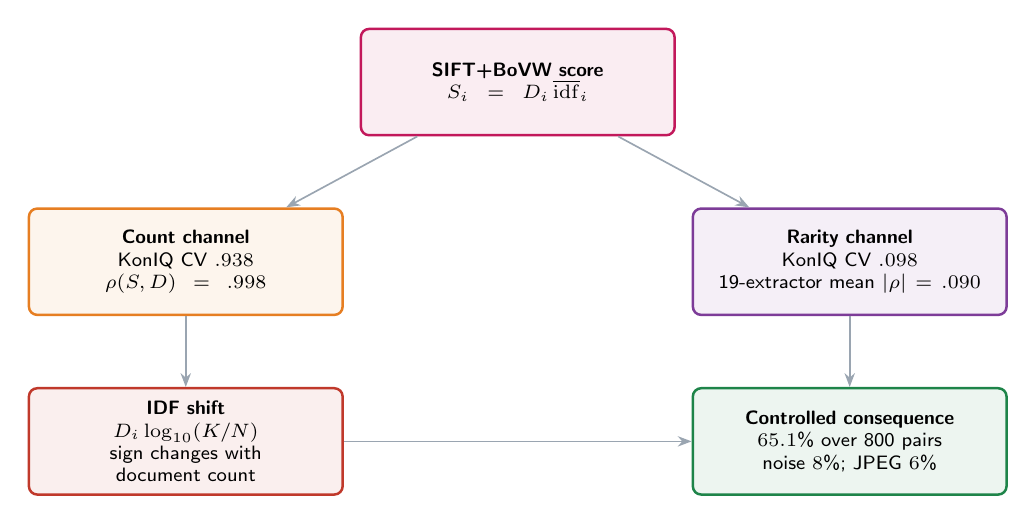
\begin{tikzpicture}[
  box/.style={rectangle,rounded corners=3pt,minimum height=1.35cm,
    text width=3.75cm,align=center,font=\sffamily\scriptsize,
    draw=#1,fill=#1!8,line width=.9pt},
  arr/.style={-{Stealth[length=5pt]},semithick,rulegray}]
\node[box=focoauditado] (score) {\textbf{SIFT+BoVW score}\\$S_i=D_i\,\overline{\mathrm{idf}}_i$};
\node[box=accentorange,below left=.9cm and .2cm of score] (count)
 {\textbf{Count channel}\\KonIQ CV $.938$\\$\rho(S,D)=.998$};
\node[box=accentpurple,below right=.9cm and .2cm of score] (rare)
 {\textbf{Rarity channel}\\KonIQ CV $.098$\\19-extractor mean $|\rho|=.090$};
\node[box=accentred,below=.9cm of count] (dep)
 {\textbf{IDF shift}\\$D_i\log_{10}(K/N)$\\sign changes with document count};
\node[box=accentgreen,below=.9cm of rare] (test)
 {\textbf{Controlled consequence}\\$65.1$\% over 800 pairs\\noise $8$\%; JPEG $6$\%};
\draw[arr] (score)--(count); \draw[arr] (score)--(rare);
\draw[arr] (count)--(dep); \draw[arr] (rare)--(test);
\draw[arr] (dep)--(test);
\end{tikzpicture}
\caption{Measured mechanism. The factorization identifies two channels; the
data determine their relative variation and connect count dominance to the
controlled-degradation failures.}
\label{fig:mechanism}
\end{figure}


\clearpage
\begin{figure}[!ht]
\centering
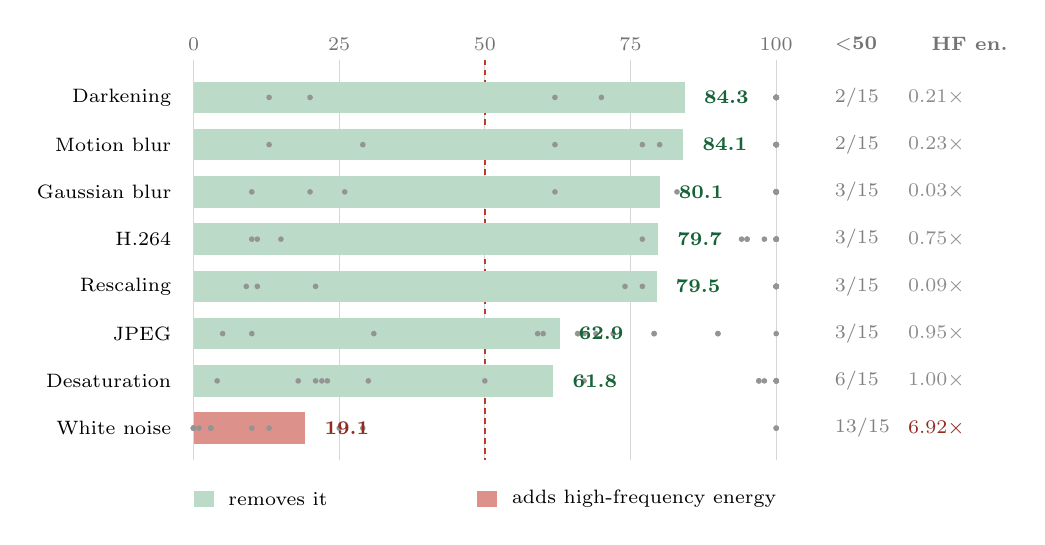
\begin{tikzpicture}[x=1cm,y=1cm,font=\scriptsize]
\draw[rulegray!45,line width=.3pt] (0.00,0.28) -- (0.00,-4.80);
\node[font=\scriptsize,text=black!55] at (0.00,0.48) {0};
\draw[rulegray!45,line width=.3pt] (1.85,0.28) -- (1.85,-4.80);
\node[font=\scriptsize,text=black!55] at (1.85,0.48) {25};
\draw[rulegray!45,line width=.3pt] (3.70,0.28) -- (3.70,-4.80);
\node[font=\scriptsize,text=black!55] at (3.70,0.48) {50};
\draw[rulegray!45,line width=.3pt] (5.55,0.28) -- (5.55,-4.80);
\node[font=\scriptsize,text=black!55] at (5.55,0.48) {75};
\draw[rulegray!45,line width=.3pt] (7.40,0.28) -- (7.40,-4.80);
\node[font=\scriptsize,text=black!55] at (7.40,0.48) {100};
\draw[accentred,line width=.8pt,dash pattern=on 2pt off 1.6pt] (3.70,0.28) -- (3.70,-4.80);
\node[anchor=east,font=\scriptsize] at (-0.16,-0.20) {Darkening};
\fill[accentgreen!30] (0,-0.40) rectangle (6.24,-0.00);
\fill[black!42] (7.40,-0.20) circle (0.036);
\fill[black!42] (7.40,-0.20) circle (0.036);
\fill[black!42] (7.40,-0.20) circle (0.036);
\fill[black!42] (7.40,-0.20) circle (0.036);
\fill[black!42] (0.96,-0.20) circle (0.036);
\fill[black!42] (7.40,-0.20) circle (0.036);
\fill[black!42] (7.40,-0.20) circle (0.036);
\fill[black!42] (5.18,-0.20) circle (0.036);
\fill[black!42] (1.48,-0.20) circle (0.036);
\fill[black!42] (7.40,-0.20) circle (0.036);
\fill[black!42] (7.40,-0.20) circle (0.036);
\fill[black!42] (7.40,-0.20) circle (0.036);
\fill[black!42] (7.40,-0.20) circle (0.036);
\fill[black!42] (4.59,-0.20) circle (0.036);
\fill[black!42] (7.40,-0.20) circle (0.036);
\node[anchor=west,font=\scriptsize\bfseries,text=accentgreen!75!black] at (6.36,-0.20) {84.3};
\node[anchor=west,font=\scriptsize,text=black!50] at (8.02,-0.20) {2/15};
\node[anchor=west,font=\scriptsize,text=black!45] at (8.95,-0.20) {0.21$\times$};
\node[anchor=east,font=\scriptsize] at (-0.16,-0.80) {Motion blur};
\fill[accentgreen!30] (0,-1.00) rectangle (6.22,-0.60);
\fill[black!42] (7.40,-0.80) circle (0.036);
\fill[black!42] (7.40,-0.80) circle (0.036);
\fill[black!42] (7.40,-0.80) circle (0.036);
\fill[black!42] (7.40,-0.80) circle (0.036);
\fill[black!42] (7.40,-0.80) circle (0.036);
\fill[black!42] (7.40,-0.80) circle (0.036);
\fill[black!42] (7.40,-0.80) circle (0.036);
\fill[black!42] (4.59,-0.80) circle (0.036);
\fill[black!42] (0.96,-0.80) circle (0.036);
\fill[black!42] (7.40,-0.80) circle (0.036);
\fill[black!42] (5.70,-0.80) circle (0.036);
\fill[black!42] (7.40,-0.80) circle (0.036);
\fill[black!42] (5.92,-0.80) circle (0.036);
\fill[black!42] (2.15,-0.80) circle (0.036);
\fill[black!42] (7.40,-0.80) circle (0.036);
\node[anchor=west,font=\scriptsize\bfseries,text=accentgreen!75!black] at (6.34,-0.80) {84.1};
\node[anchor=west,font=\scriptsize,text=black!50] at (8.02,-0.80) {2/15};
\node[anchor=west,font=\scriptsize,text=black!45] at (8.95,-0.80) {0.23$\times$};
\node[anchor=east,font=\scriptsize] at (-0.16,-1.40) {Gaussian blur};
\fill[accentgreen!30] (0,-1.60) rectangle (5.92,-1.20);
\fill[black!42] (7.40,-1.40) circle (0.036);
\fill[black!42] (7.40,-1.40) circle (0.036);
\fill[black!42] (7.40,-1.40) circle (0.036);
\fill[black!42] (7.40,-1.40) circle (0.036);
\fill[black!42] (7.40,-1.40) circle (0.036);
\fill[black!42] (7.40,-1.40) circle (0.036);
\fill[black!42] (7.40,-1.40) circle (0.036);
\fill[black!42] (4.59,-1.40) circle (0.036);
\fill[black!42] (0.74,-1.40) circle (0.036);
\fill[black!42] (7.40,-1.40) circle (0.036);
\fill[black!42] (6.14,-1.40) circle (0.036);
\fill[black!42] (7.40,-1.40) circle (0.036);
\fill[black!42] (1.92,-1.40) circle (0.036);
\fill[black!42] (1.48,-1.40) circle (0.036);
\fill[black!42] (7.40,-1.40) circle (0.036);
\node[anchor=west,font=\scriptsize\bfseries,text=accentgreen!75!black] at (6.04,-1.40) {80.1};
\node[anchor=west,font=\scriptsize,text=black!50] at (8.02,-1.40) {3/15};
\node[anchor=west,font=\scriptsize,text=black!45] at (8.95,-1.40) {0.03$\times$};
\node[anchor=east,font=\scriptsize] at (-0.16,-2.00) {H.264};
\fill[accentgreen!30] (0,-2.20) rectangle (5.90,-1.80);
\fill[black!42] (7.40,-2.00) circle (0.036);
\fill[black!42] (7.40,-2.00) circle (0.036);
\fill[black!42] (7.40,-2.00) circle (0.036);
\fill[black!42] (7.40,-2.00) circle (0.036);
\fill[black!42] (1.11,-2.00) circle (0.036);
\fill[black!42] (7.40,-2.00) circle (0.036);
\fill[black!42] (7.25,-2.00) circle (0.036);
\fill[black!42] (0.81,-2.00) circle (0.036);
\fill[black!42] (5.70,-2.00) circle (0.036);
\fill[black!42] (7.03,-2.00) circle (0.036);
\fill[black!42] (0.74,-2.00) circle (0.036);
\fill[black!42] (7.40,-2.00) circle (0.036);
\fill[black!42] (7.03,-2.00) circle (0.036);
\fill[black!42] (6.96,-2.00) circle (0.036);
\fill[black!42] (7.40,-2.00) circle (0.036);
\node[anchor=west,font=\scriptsize\bfseries,text=accentgreen!75!black] at (6.02,-2.00) {79.7};
\node[anchor=west,font=\scriptsize,text=black!50] at (8.02,-2.00) {3/15};
\node[anchor=west,font=\scriptsize,text=black!45] at (8.95,-2.00) {0.75$\times$};
\node[anchor=east,font=\scriptsize] at (-0.16,-2.60) {Rescaling};
\fill[accentgreen!30] (0,-2.80) rectangle (5.88,-2.40);
\fill[black!42] (7.40,-2.60) circle (0.036);
\fill[black!42] (7.40,-2.60) circle (0.036);
\fill[black!42] (7.40,-2.60) circle (0.036);
\fill[black!42] (7.40,-2.60) circle (0.036);
\fill[black!42] (7.40,-2.60) circle (0.036);
\fill[black!42] (7.40,-2.60) circle (0.036);
\fill[black!42] (7.40,-2.60) circle (0.036);
\fill[black!42] (5.48,-2.60) circle (0.036);
\fill[black!42] (0.81,-2.60) circle (0.036);
\fill[black!42] (7.40,-2.60) circle (0.036);
\fill[black!42] (5.70,-2.60) circle (0.036);
\fill[black!42] (7.40,-2.60) circle (0.036);
\fill[black!42] (0.67,-2.60) circle (0.036);
\fill[black!42] (1.55,-2.60) circle (0.036);
\fill[black!42] (7.40,-2.60) circle (0.036);
\node[anchor=west,font=\scriptsize\bfseries,text=accentgreen!75!black] at (6.00,-2.60) {79.5};
\node[anchor=west,font=\scriptsize,text=black!50] at (8.02,-2.60) {3/15};
\node[anchor=west,font=\scriptsize,text=black!45] at (8.95,-2.60) {0.09$\times$};
\node[anchor=east,font=\scriptsize] at (-0.16,-3.20) {JPEG};
\fill[accentgreen!30] (0,-3.40) rectangle (4.65,-3.00);
\fill[black!42] (6.66,-3.20) circle (0.036);
\fill[black!42] (5.33,-3.20) circle (0.036);
\fill[black!42] (4.96,-3.20) circle (0.036);
\fill[black!42] (5.85,-3.20) circle (0.036);
\fill[black!42] (6.66,-3.20) circle (0.036);
\fill[black!42] (5.85,-3.20) circle (0.036);
\fill[black!42] (4.44,-3.20) circle (0.036);
\fill[black!42] (2.29,-3.20) circle (0.036);
\fill[black!42] (4.37,-3.20) circle (0.036);
\fill[black!42] (4.88,-3.20) circle (0.036);
\fill[black!42] (4.88,-3.20) circle (0.036);
\fill[black!42] (0.37,-3.20) circle (0.036);
\fill[black!42] (7.40,-3.20) circle (0.036);
\fill[black!42] (0.74,-3.20) circle (0.036);
\fill[black!42] (5.11,-3.20) circle (0.036);
\node[anchor=west,font=\scriptsize\bfseries,text=accentgreen!75!black] at (4.77,-3.20) {62.9};
\node[anchor=west,font=\scriptsize,text=black!50] at (8.02,-3.20) {3/15};
\node[anchor=west,font=\scriptsize,text=black!45] at (8.95,-3.20) {0.95$\times$};
\node[anchor=east,font=\scriptsize] at (-0.16,-3.80) {Desaturation};
\fill[accentgreen!30] (0,-4.00) rectangle (4.57,-3.60);
\fill[black!42] (1.63,-3.80) circle (0.036);
\fill[black!42] (4.96,-3.80) circle (0.036);
\fill[black!42] (7.40,-3.80) circle (0.036);
\fill[black!42] (7.40,-3.80) circle (0.036);
\fill[black!42] (7.40,-3.80) circle (0.036);
\fill[black!42] (7.40,-3.80) circle (0.036);
\fill[black!42] (2.22,-3.80) circle (0.036);
\fill[black!42] (7.18,-3.80) circle (0.036);
\fill[black!42] (0.30,-3.80) circle (0.036);
\fill[black!42] (3.70,-3.80) circle (0.036);
\fill[black!42] (7.18,-3.80) circle (0.036);
\fill[black!42] (1.70,-3.80) circle (0.036);
\fill[black!42] (1.55,-3.80) circle (0.036);
\fill[black!42] (1.33,-3.80) circle (0.036);
\fill[black!42] (7.25,-3.80) circle (0.036);
\node[anchor=west,font=\scriptsize\bfseries,text=accentgreen!75!black] at (4.69,-3.80) {61.8};
\node[anchor=west,font=\scriptsize,text=black!50] at (8.02,-3.80) {6/15};
\node[anchor=west,font=\scriptsize,text=black!45] at (8.95,-3.80) {1.00$\times$};
\node[anchor=east,font=\scriptsize] at (-0.16,-4.40) {White noise};
\fill[accentred!55] (0,-4.60) rectangle (1.42,-4.20);
\fill[black!42] (1.85,-4.40) circle (0.036);
\fill[black!42] (0.00,-4.40) circle (0.036);
\fill[black!42] (0.22,-4.40) circle (0.036);
\fill[black!42] (0.22,-4.40) circle (0.036);
\fill[black!42] (0.07,-4.40) circle (0.036);
\fill[black!42] (0.22,-4.40) circle (0.036);
\fill[black!42] (0.74,-4.40) circle (0.036);
\fill[black!42] (7.40,-4.40) circle (0.036);
\fill[black!42] (7.40,-4.40) circle (0.036);
\fill[black!42] (0.00,-4.40) circle (0.036);
\fill[black!42] (0.00,-4.40) circle (0.036);
\fill[black!42] (0.00,-4.40) circle (0.036);
\fill[black!42] (0.00,-4.40) circle (0.036);
\fill[black!42] (0.96,-4.40) circle (0.036);
\fill[black!42] (2.15,-4.40) circle (0.036);
\node[anchor=west,font=\scriptsize\bfseries,text=accentred!75!black] at (1.54,-4.40) {19.1};
\node[anchor=west,font=\scriptsize,text=black!50] at (8.02,-4.40) {13/15};
\node[anchor=west,font=\scriptsize,text=accentred!75!black] at (8.95,-4.40) {6.92$\times$};
\node[anchor=west,font=\scriptsize\bfseries,text=black!55] at (8.02,0.48) {$<$50};
\node[anchor=west,font=\scriptsize\bfseries,text=black!55] at (9.25,0.48) {HF en.};
\fill[accentgreen!30] (0,-5.40) rectangle (0.26,-5.20);
\node[anchor=west,font=\scriptsize] at (0.32,-5.30) {removes it};
\fill[accentred!55] (3.6,-5.40) rectangle (3.86,-5.20);
\node[anchor=west,font=\scriptsize] at (3.92,-5.30) {adds high-frequency energy};
\end{tikzpicture}
\caption{Mean paired accuracy of the fifteen summarization operations, by degradation type; grey dots are the individual operations and the dashed line is chance. \textbf{Rows are ordered by mean accuracy, descending.} The last column is what each degradation does to local image high-frequency energy, measured as the median ratio to the original. For the Seven transformations that reduce it, mean paired accuracy exceeds 50 per cent and the displayed median ratio is at most 1.00. \textbf{White noise is the only one that raises it}, by a factor of $6.9$, and it is answered at $19.1$ per cent with a median of $3.0$. The middle column counts operations below chance.}
\label{fig:direction}
\end{figure}


\clearpage
\begin{table}[!ht]
\centering
\caption{Model-reference output over the 42 operational redundancy clusters.
Changed counts representatives differing from the SIFT+BoVW operation. DOVER-T
is the raw DOVER technical branch and is not used in screening; Q-Align defines
the in-domain screening floor. Both outputs use the global-achievable-range
estimand of Eq.~2 of the main article; Max is the percentage of clusters in which
the selected representative has the highest DOVER-T score.}
\label{tab:e2e}
\small
\setlength{\tabcolsep}{5pt}
\renewcommand{\arraystretch}{1.08}
\begin{tabular}{@{}lcrrr@{}}
\toprule
\rowcolor{headerblue}
\hd{Quality operation} & \hd{Changed} & \hd{DOVER-T} & \hd{Max} & \hd{Q-Align} \\
\midrule
\rowcolor{focoauditado!12}SIFT+BoVW & --- & 50.5\% & 54.8\% & 48.6\% \\
\rowcolor{accentgreen!15}\textbf{LIQE} & \textbf{22/42} & \textbf{76.0\%} & 59.5\% & 90.2\% \\
QualiCLIP & 19/42 & 71.9\% & 59.5\% & 80.6\% \\
\rowcolor{rowlight}CLIP-IQA$+$ & 22/42 & 70.7\% & 50.0\% & 74.3\% \\
\bottomrule
\end{tabular}
\end{table}


\clearpage
\begin{table}[!ht]
\centering
\caption{Complete-case method screening. Sensitivity reports the within-reference
mean and number of KADID types above .50. Generalization is the lowest signed
$\rho^{*}$ over all unseen databases. Floor is normalized agreement with Q-Align
on the common 42 clusters and its lower bound (L) under the \senBlocos{} separate topic
labels, \textbf{which is the sensitivity grouping}: the primary interval of Section~4.5
of the main text resamples the \fusBlocos{} source-aware blocks and gives \finLiqe{}
for LIQE Sup.: K =
KonIQ-10k opinion training; L = LIVE; OU = opinion-unaware; -- = no opinion
training; M = multi-database mixture. A dagger marks a value measured on a database the method trained on: Q-Align's mixture includes KADID-10k. Q-Align is a reference, not a candidate.}
\label{tab:screening}
\scriptsize
\setlength{\tabcolsep}{1.7pt}
\renewcommand{\arraystretch}{1.08}
\begin{tabular}{@{}lcccccc@{}}
\toprule
\rowcolor{headerblue}
\hd{Method} & \hd{Sup.} & \hd{Pol.} & \hd{Sensitivity} &
\hd{Lowest unseen $\rho^{*}$} & \hd{Floor; L} & \hd{Eligible} \\
\midrule
\rowcolor{accentgreen!15}\textbf{LIQE} & K & \polup & .807; 22 & .723 & .551; .284 & \textbf{yes} \\
\rowcolor{accentgreen!15}\textbf{QualiCLIP} & OU & \polup & .849; 22 & .665 & .371; .143 & \textbf{yes} \\
\rowcolor{accentgreen!15}\textbf{CLIP-IQA$+$} & K & \polup & .808; 22 & .654 & .236; .034 & \textbf{yes} \\
\midrule
TOPIQ & K & \polup & .721; 20 & .511 & .506; .289 & no \\
\rowcolor{rowlight}MUSIQ & K & \polup & .733; 20 & .556 & .551; .297 & no \\
DBCNN & K & \polup & .668; 19 & .484 & .461; .274 & no \\
\rowcolor{rowlight}HyperIQA & K & \polup & .673; 19 & .462 & .371; .122 & no \\
NIQE & OU & \poldown & .607; 19 & .368 & .281; .012 & no \\
\rowcolor{rowlight}BRISQUE & L & \poldown & .657; 19 & .236 & .371; .136 & no \\
CLIP-IQA & OU & \polup & .645; 20 & .501 & .371; .045 & no \\
\rowcolor{focoauditado!12}SIFT+BoVW & -- & \polup & $-.077$; 5 & $-.445$ & .056; $-.308$ & no \\
\midrule
\rowcolor{rowlight}Q-Align & M & \polup & .880$^{\dagger}$; 23$^{\dagger}$ & -- & -- & reference \\
\bottomrule
\end{tabular}
\end{table}


\clearpage
\begin{table}[!ht]
\centering
\caption{Two published expressions against the property the same paragraph claims for them. \textbf{Above}: the contrast term of the Qaroush visual-attention objective, over a sweep in which contrast rises by construction (25 levels, seed 42). Histogram equalisation raises the standard deviation of every frame in this sweep. Over it, the published form and the form without the absolute value are both perfectly inversely associated with the measure used to build the inputs; only the ratio, which the equation does not write, is perfectly positively associated. \textbf{Below}: the brightness term of the Korolkov module, over a sweep in which exposure rises by construction (21 levels). The source states that it ``penalizes under- and over-exposed frames'', which requires a non-monotone function; the mean luminance it specifies is monotone and enters the module with weight $+0.3$, so a brighter frame always scores higher. \textbf{No corpus is involved.} The Korolkov inversion follows from the expression; the Qaroush result is the behaviour of the expression over this sweep.}
\label{tab:ct}
\footnotesize
\setlength{\tabcolsep}{3.5pt}
\renewcommand{\arraystretch}{1.35}
\begin{tabular}{@{}>{\raggedright\arraybackslash}p{4.0cm} l r@{}}
\toprule
\rowcolor{headerblue}
\hd{Reading} & \hd{Expression} & \hd{$\rho$ with the property} \\
\midrule
\multicolumn{3}{@{}l}{\textit{Qaroush contrast, against contrast (Eq.~8)}} \\
\quad Eq.~8 as published & $\frac{1}{K}\sum_k\bigl|\sigma_p(\mathrm{HE}(f_k))-\sigma_p(f_k)\bigr|$ & \textcolor{accentred}{\textbf{$-1.0000$}} \\
\rowcolor{rowlight}\quad without the absolute value & $\frac{1}{K}\sum_k\bigl(\sigma_p(\mathrm{HE}(f_k))-\sigma_p(f_k)\bigr)$ & \textcolor{accentred}{\textbf{$-1.0000$}} \\
\quad ratio, unwritten in the source & $\frac{1}{K}\sum_k \sigma_p(f_k)/\sigma_p(\mathrm{HE}(f_k))$ & $+1.0000$ \\
\midrule
\multicolumn{3}{@{}l}{\textit{Korolkov brightness, against exposure}} \\
\quad as published & $\frac{1}{|I|}\sum_{x,y} L(I)_{x,y}$ (LAB) & $+1.0000$ \\
\rowcolor{rowlight}\quad illustrative non-monotone penalty & $-\bigl|L-127.5\bigr|$ & \textcolor{accentred}{\textbf{$-.4883$}} \\
\bottomrule
\end{tabular}
\end{table}


\clearpage
\begin{table}[!ht]
\centering
\caption{Traceability of every audited operation: the source work, the formula as the source states it, the function that computes it, and the reference model used on the in-domain column. Every operation name and count printed elsewhere in this article is derived from this table. \textbf{Dir.} is the direction the source declares; spatial information declares none, which is why it is measured but carries no verdict. \textbf{A superscript marks fidelity}: $^{\mathrm{a}}$ adapted input, $^{\mathrm{b}}$ expression not stated by the source, $^{\mathrm{c}}$ combination chosen here, $^{\mathrm{d}}$ adapted normalization; unmarked is the source expression, unadapted. \textbf{A marked row characterizes that variant, not the complete source system.}}
\label{tab:trace}
\scriptsize
\setlength{\tabcolsep}{3.4pt}
\renewcommand{\arraystretch}{1.02}
\begin{tabular}{@{}>{\raggedright\arraybackslash}p{2.15cm}>{\raggedright\arraybackslash}p{1.95cm}>{\raggedright\arraybackslash}p{3.70cm}>{\raggedright\arraybackslash}p{2.55cm}c c@{}}
\toprule
\rowcolor{headerblue}
\hd{Operation} & \hd{Source} & \hd{Formula, as the source states it} & \hd{Function in code} & \hd{Dir.} & \hd{Ref.} \\
\midrule
Averaged aesthetics (3)$^{\mathrm{c}}$ & \citep{gygli2014summe} & three aesthetic attributes; unweighted mean$^{\ddagger}$ & \texttt{gygli\_\allowbreak{}media\_\allowbreak{}crua} & $\uparrow$ & LIQE \\
\rowcolor{rowlight}Colourfulness (Hasler) & \citep{hasler2003colorfulness} & $M^{(3)}=\sigma_{rgyb}+.3\mu_{rgyb}$ & \texttt{hasler\_\allowbreak{}colorfulness} & $\uparrow$ & LIQE \\
Colourfulness (Ke)$^{\mathrm{b}}$ & \citep{ke2006highlevel} & Hasler $M^{(3)}$; Ke gives no formula & \texttt{hasler\_\allowbreak{}colorfulness} & $\uparrow$ & LIQE \\
\rowcolor{rowlight}Composite of five$^{\mathrm{d}}$ & \citep{srinivas2016rank}, \citep{ke2006highlevel} & unweighted mean of the five Ke terms & \texttt{srinivas\_\allowbreak{}quality} & $\uparrow$ & LIQE \\
Contrast & \citep{ke2006highlevel} & width of central 98\% of the grey histogram (Ke \S4.5) & \texttt{ke\_\allowbreak{}contraste} & $\uparrow$ & LIQE \\
\rowcolor{rowlight}Edge distribution$^{\mathrm{a}}$ & \citep{ke2006highlevel} & $q_a=1-w_xw_y$ (Ke \S4.1)$^{\P}$ & \texttt{ke\_\allowbreak{}edge\_\allowbreak{}distribution} & $\uparrow$ & LIQE \\
Entropy & \citep{qaroush2025diversity} & Shannon entropy over HSV histogram bins (Eq.~5) & \texttt{qaroush\_\allowbreak{}entropia} & $\uparrow$ & LIQE \\
\rowcolor{rowlight}GLCM contrast & \citep{yang2024keyframe} & GLCM contrast descriptor & \texttt{glcm\_\allowbreak{}contraste} & $\uparrow$ & LIQE \\
Gradient magnitude & \citep{qaroush2025diversity} & mean Sobel gradient magnitude (Eq.~10) & \texttt{qaroush\_\allowbreak{}gm} & $\uparrow$ & LIQE \\
\rowcolor{rowlight}Gradient orientation & \citep{qaroush2025diversity} & SD of Sobel gradient orientations (Eq.~15) & \texttt{qaroush\_\allowbreak{}go} & $\uparrow$ & LIQE \\
Grey-level dispersion$^{\S}$ & \citep{jeong2016static}, \citep{xu2024property} & grey-level standard deviation & \texttt{contraste\_\allowbreak{}variancia} & $\uparrow$ & LIQE \\
\rowcolor{rowlight}Hue count & \citep{ke2006highlevel} & $q_h=20-|N|$, $\alpha=.05$ (Ke \S4.3) & \texttt{ke\_\allowbreak{}hue\_\allowbreak{}count} & $\uparrow$ & LIQE \\
Laplacian variance & \citep{cakmak2025tripss}, \citep{korolkov2025keyframe} & variance of the grey-scale Laplacian & \texttt{laplacian\_\allowbreak{}var} & $\uparrow$ & LIQE \\
\rowcolor{rowlight}Saliency area$^{\mathrm{a}}$ & \citep{qaroush2025diversity} & area fraction above a saliency threshold (Eq.~6)$^{\mathsection\mathsection}$ & \texttt{qaroush\_\allowbreak{}saliencia} & $\uparrow$ & LIQE \\
Saturation & \citep{huang2024aesthetic} & mean HSV saturation (\S III-A-1) & \texttt{huang\_\allowbreak{}saturacao} & $\uparrow$ & LIQE \\
\rowcolor{rowlight}Spatial information & \citep{itu_p910} & Sobel energy, ITU-T P.910 & \texttt{si} & \textcolor{black!45}{none} & LIQE \\
\bottomrule
\end{tabular}
\end{table}
\FloatBarrier

\noindent\begin{minipage}{\linewidth}\scriptsize\textbf{Notes to Table~\ref{tab:trace}.} All sixteen are computed by \texttt{ops\_da\_literatura.py} on the same frames and pooled identically. \textbf{Ref.} is the model each operation is compared against on the in-domain column; the ten no-reference models in the main screening table use Q-Align there instead, so that column compares each family with its own reference. Colourfulness has no formula in Ke, who cites Datta; the Hasler expression is used as an explicitly documented substitution. Scores for fifteen operations are in \texttt{corpus\_inteiro.json}; spatial information is scored on the extended 83-segment design by \texttt{si\_no\_corpus\_de\_video}, in \texttt{designA\_estendido\_83.json}.\par\smallskip
$^{\ddagger}$\,Ref.~\citep{gygli2014summe} lists the attributes but not their combination; \textbf{the unweighted mean is a choice made here}. $^{\mathsection\mathsection}$\,Spectral-residual map~\citep{hou2007spectral}, not the learned backbone the source prescribes. $^{\P}$\,Ke builds the edge map with a Laplacian per RGB channel at $100\times100$; here it is Sobel magnitude on the grey frame. $^{\S}$\,Ref.~\citep{jeong2016static} states \emph{variance of pixels} and Ref.~\citep{xu2024property} \emph{the mean difference and standard deviation of the grayscale values}; \textbf{only the standard deviation is implemented}.\end{minipage}\par\medskip

\noindent\begin{minipage}{\linewidth}\scriptsize \textbf{Implementation controls.} With the source edge map of Ke, sensitivity goes 0.298$\to$0.272 and types 9$\to$7 (the two versions correlate 0.876); no verdict changes. \textbf{Within a frame the variance and the standard deviation order alike; a mean over frames does not}: under the mean of variances 7 of the 800 pairs move and no per-type verdict does.\end{minipage}\par\medskip


\begin{figure}[!ht]
\centering
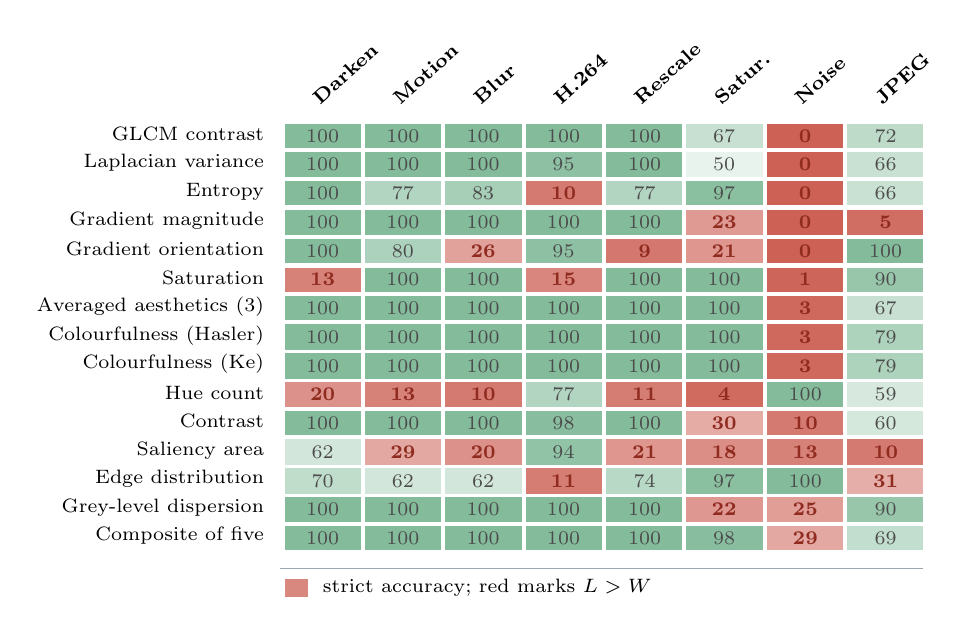
\begin{tikzpicture}[x=1cm,y=1cm,font=\scriptsize]
\node[rotate=42,anchor=west,font=\scriptsize\bfseries] at (0.30,0.16) {Darken};
\node[rotate=42,anchor=west,font=\scriptsize\bfseries] at (1.32,0.16) {Motion};
\node[rotate=42,anchor=west,font=\scriptsize\bfseries] at (2.34,0.16) {Blur};
\node[rotate=42,anchor=west,font=\scriptsize\bfseries] at (3.36,0.16) {H.264};
\node[rotate=42,anchor=west,font=\scriptsize\bfseries] at (4.38,0.16) {Rescale};
\node[rotate=42,anchor=west,font=\scriptsize\bfseries] at (5.40,0.16) {Satur.};
\node[rotate=42,anchor=west,font=\scriptsize\bfseries] at (6.42,0.16) {Noise};
\node[rotate=42,anchor=west,font=\scriptsize\bfseries] at (7.44,0.16) {JPEG};
\node[anchor=east,font=\scriptsize] at (-0.14,-0.18) {GLCM contrast};
\fill[accentgreen!55] (0.00,-0.36) rectangle (0.97,-0.05);
\node[font=\scriptsize,text=black!70] at (0.48,-0.21) {100};
\fill[accentgreen!55] (1.02,-0.36) rectangle (1.99,-0.05);
\node[font=\scriptsize,text=black!70] at (1.50,-0.21) {100};
\fill[accentgreen!55] (2.04,-0.36) rectangle (3.01,-0.05);
\node[font=\scriptsize,text=black!70] at (2.52,-0.21) {100};
\fill[accentgreen!55] (3.06,-0.36) rectangle (4.03,-0.05);
\node[font=\scriptsize,text=black!70] at (3.54,-0.21) {100};
\fill[accentgreen!55] (4.08,-0.36) rectangle (5.05,-0.05);
\node[font=\scriptsize,text=black!70] at (4.57,-0.21) {100};
\fill[accentgreen!25] (5.10,-0.36) rectangle (6.07,-0.05);
\node[font=\scriptsize,text=black!70] at (5.58,-0.21) {67};
\fill[accentred!80] (6.12,-0.36) rectangle (7.09,-0.05);
\node[font=\scriptsize\bfseries,text=accentred!75!black] at (6.61,-0.21) {0};
\fill[accentgreen!29] (7.14,-0.36) rectangle (8.11,-0.05);
\node[font=\scriptsize,text=black!70] at (7.63,-0.21) {72};
\node[anchor=east,font=\scriptsize] at (-0.14,-0.55) {Laplacian variance};
\fill[accentgreen!55] (0.00,-0.73) rectangle (0.97,-0.41);
\node[font=\scriptsize,text=black!70] at (0.48,-0.57) {100};
\fill[accentgreen!55] (1.02,-0.73) rectangle (1.99,-0.41);
\node[font=\scriptsize,text=black!70] at (1.50,-0.57) {100};
\fill[accentgreen!55] (2.04,-0.73) rectangle (3.01,-0.41);
\node[font=\scriptsize,text=black!70] at (2.52,-0.57) {100};
\fill[accentgreen!50] (3.06,-0.73) rectangle (4.03,-0.41);
\node[font=\scriptsize,text=black!70] at (3.54,-0.57) {95};
\fill[accentgreen!55] (4.08,-0.73) rectangle (5.05,-0.41);
\node[font=\scriptsize,text=black!70] at (4.57,-0.57) {100};
\fill[accentgreen!10] (5.10,-0.73) rectangle (6.07,-0.41);
\node[font=\scriptsize,text=black!70] at (5.58,-0.57) {50};
\fill[accentred!80] (6.12,-0.73) rectangle (7.09,-0.41);
\node[font=\scriptsize\bfseries,text=accentred!75!black] at (6.61,-0.57) {0};
\fill[accentgreen!24] (7.14,-0.73) rectangle (8.11,-0.41);
\node[font=\scriptsize,text=black!70] at (7.63,-0.57) {66};
\node[anchor=east,font=\scriptsize] at (-0.14,-0.91) {Entropy};
\fill[accentgreen!55] (0.00,-1.09) rectangle (0.97,-0.78);
\node[font=\scriptsize,text=black!70] at (0.48,-0.94) {100};
\fill[accentgreen!34] (1.02,-1.09) rectangle (1.99,-0.78);
\node[font=\scriptsize,text=black!70] at (1.50,-0.94) {77};
\fill[accentgreen!39] (2.04,-1.09) rectangle (3.01,-0.78);
\node[font=\scriptsize,text=black!70] at (2.52,-0.94) {83};
\fill[accentred!67] (3.06,-1.09) rectangle (4.03,-0.78);
\node[font=\scriptsize\bfseries,text=accentred!75!black] at (3.54,-0.94) {10};
\fill[accentgreen!34] (4.08,-1.09) rectangle (5.05,-0.78);
\node[font=\scriptsize,text=black!70] at (4.57,-0.94) {77};
\fill[accentgreen!52] (5.10,-1.09) rectangle (6.07,-0.78);
\node[font=\scriptsize,text=black!70] at (5.58,-0.94) {97};
\fill[accentred!80] (6.12,-1.09) rectangle (7.09,-0.78);
\node[font=\scriptsize\bfseries,text=accentred!75!black] at (6.61,-0.94) {0};
\fill[accentgreen!24] (7.14,-1.09) rectangle (8.11,-0.78);
\node[font=\scriptsize,text=black!70] at (7.63,-0.94) {66};
\node[anchor=east,font=\scriptsize] at (-0.14,-1.28) {Gradient magnitude};
\fill[accentgreen!55] (0.00,-1.46) rectangle (0.97,-1.15);
\node[font=\scriptsize,text=black!70] at (0.48,-1.30) {100};
\fill[accentgreen!55] (1.02,-1.46) rectangle (1.99,-1.15);
\node[font=\scriptsize,text=black!70] at (1.50,-1.30) {100};
\fill[accentgreen!55] (2.04,-1.46) rectangle (3.01,-1.15);
\node[font=\scriptsize,text=black!70] at (2.52,-1.30) {100};
\fill[accentgreen!55] (3.06,-1.46) rectangle (4.03,-1.15);
\node[font=\scriptsize,text=black!70] at (3.54,-1.30) {100};
\fill[accentgreen!55] (4.08,-1.46) rectangle (5.05,-1.15);
\node[font=\scriptsize,text=black!70] at (4.57,-1.30) {100};
\fill[accentred!51] (5.10,-1.46) rectangle (6.07,-1.15);
\node[font=\scriptsize\bfseries,text=accentred!75!black] at (5.58,-1.30) {23};
\fill[accentred!80] (6.12,-1.46) rectangle (7.09,-1.15);
\node[font=\scriptsize\bfseries,text=accentred!75!black] at (6.61,-1.30) {0};
\fill[accentred!73] (7.14,-1.46) rectangle (8.11,-1.15);
\node[font=\scriptsize\bfseries,text=accentred!75!black] at (7.63,-1.30) {5};
\node[anchor=east,font=\scriptsize] at (-0.14,-1.64) {Gradient orientation};
\fill[accentgreen!55] (0.00,-1.82) rectangle (0.97,-1.51);
\node[font=\scriptsize,text=black!70] at (0.48,-1.67) {100};
\fill[accentgreen!37] (1.02,-1.82) rectangle (1.99,-1.51);
\node[font=\scriptsize,text=black!70] at (1.50,-1.67) {80};
\fill[accentred!47] (2.04,-1.82) rectangle (3.01,-1.51);
\node[font=\scriptsize\bfseries,text=accentred!75!black] at (2.52,-1.67) {26};
\fill[accentgreen!50] (3.06,-1.82) rectangle (4.03,-1.51);
\node[font=\scriptsize,text=black!70] at (3.54,-1.67) {95};
\fill[accentred!68] (4.08,-1.82) rectangle (5.05,-1.51);
\node[font=\scriptsize\bfseries,text=accentred!75!black] at (4.57,-1.67) {9};
\fill[accentred!53] (5.10,-1.82) rectangle (6.07,-1.51);
\node[font=\scriptsize\bfseries,text=accentred!75!black] at (5.58,-1.67) {21};
\fill[accentred!80] (6.12,-1.82) rectangle (7.09,-1.51);
\node[font=\scriptsize\bfseries,text=accentred!75!black] at (6.61,-1.67) {0};
\fill[accentgreen!55] (7.14,-1.82) rectangle (8.11,-1.51);
\node[font=\scriptsize,text=black!70] at (7.63,-1.67) {100};
\node[anchor=east,font=\scriptsize] at (-0.14,-2.01) {Saturation};
\fill[accentred!63] (0.00,-2.19) rectangle (0.97,-1.88);
\node[font=\scriptsize\bfseries,text=accentred!75!black] at (0.48,-2.03) {13};
\fill[accentgreen!55] (1.02,-2.19) rectangle (1.99,-1.88);
\node[font=\scriptsize,text=black!70] at (1.50,-2.03) {100};
\fill[accentgreen!55] (2.04,-2.19) rectangle (3.01,-1.88);
\node[font=\scriptsize,text=black!70] at (2.52,-2.03) {100};
\fill[accentred!61] (3.06,-2.19) rectangle (4.03,-1.88);
\node[font=\scriptsize\bfseries,text=accentred!75!black] at (3.54,-2.03) {15};
\fill[accentgreen!55] (4.08,-2.19) rectangle (5.05,-1.88);
\node[font=\scriptsize,text=black!70] at (4.57,-2.03) {100};
\fill[accentgreen!55] (5.10,-2.19) rectangle (6.07,-1.88);
\node[font=\scriptsize,text=black!70] at (5.58,-2.03) {100};
\fill[accentred!78] (6.12,-2.19) rectangle (7.09,-1.88);
\node[font=\scriptsize\bfseries,text=accentred!75!black] at (6.61,-2.03) {1};
\fill[accentgreen!46] (7.14,-2.19) rectangle (8.11,-1.88);
\node[font=\scriptsize,text=black!70] at (7.63,-2.03) {90};
\node[anchor=east,font=\scriptsize] at (-0.14,-2.37) {Averaged aesthetics (3)};
\fill[accentgreen!55] (0.00,-2.55) rectangle (0.97,-2.24);
\node[font=\scriptsize,text=black!70] at (0.48,-2.40) {100};
\fill[accentgreen!55] (1.02,-2.55) rectangle (1.99,-2.24);
\node[font=\scriptsize,text=black!70] at (1.50,-2.40) {100};
\fill[accentgreen!55] (2.04,-2.55) rectangle (3.01,-2.24);
\node[font=\scriptsize,text=black!70] at (2.52,-2.40) {100};
\fill[accentgreen!55] (3.06,-2.55) rectangle (4.03,-2.24);
\node[font=\scriptsize,text=black!70] at (3.54,-2.40) {100};
\fill[accentgreen!55] (4.08,-2.55) rectangle (5.05,-2.24);
\node[font=\scriptsize,text=black!70] at (4.57,-2.40) {100};
\fill[accentgreen!55] (5.10,-2.55) rectangle (6.07,-2.24);
\node[font=\scriptsize,text=black!70] at (5.58,-2.40) {100};
\fill[accentred!76] (6.12,-2.55) rectangle (7.09,-2.24);
\node[font=\scriptsize\bfseries,text=accentred!75!black] at (6.61,-2.40) {3};
\fill[accentgreen!25] (7.14,-2.55) rectangle (8.11,-2.24);
\node[font=\scriptsize,text=black!70] at (7.63,-2.40) {67};
\node[anchor=east,font=\scriptsize] at (-0.14,-2.74) {Colourfulness (Hasler)};
\fill[accentgreen!55] (0.00,-2.92) rectangle (0.97,-2.60);
\node[font=\scriptsize,text=black!70] at (0.48,-2.76) {100};
\fill[accentgreen!55] (1.02,-2.92) rectangle (1.99,-2.60);
\node[font=\scriptsize,text=black!70] at (1.50,-2.76) {100};
\fill[accentgreen!55] (2.04,-2.92) rectangle (3.01,-2.60);
\node[font=\scriptsize,text=black!70] at (2.52,-2.76) {100};
\fill[accentgreen!55] (3.06,-2.92) rectangle (4.03,-2.60);
\node[font=\scriptsize,text=black!70] at (3.54,-2.76) {100};
\fill[accentgreen!55] (4.08,-2.92) rectangle (5.05,-2.60);
\node[font=\scriptsize,text=black!70] at (4.57,-2.76) {100};
\fill[accentgreen!55] (5.10,-2.92) rectangle (6.07,-2.60);
\node[font=\scriptsize,text=black!70] at (5.58,-2.76) {100};
\fill[accentred!76] (6.12,-2.92) rectangle (7.09,-2.60);
\node[font=\scriptsize\bfseries,text=accentred!75!black] at (6.61,-2.76) {3};
\fill[accentgreen!36] (7.14,-2.92) rectangle (8.11,-2.60);
\node[font=\scriptsize,text=black!70] at (7.63,-2.76) {79};
\node[anchor=east,font=\scriptsize] at (-0.14,-3.10) {Colourfulness (Ke)};
\fill[accentgreen!55] (0.00,-3.29) rectangle (0.97,-2.97);
\node[font=\scriptsize,text=black!70] at (0.48,-3.13) {100};
\fill[accentgreen!55] (1.02,-3.29) rectangle (1.99,-2.97);
\node[font=\scriptsize,text=black!70] at (1.50,-3.13) {100};
\fill[accentgreen!55] (2.04,-3.29) rectangle (3.01,-2.97);
\node[font=\scriptsize,text=black!70] at (2.52,-3.13) {100};
\fill[accentgreen!55] (3.06,-3.29) rectangle (4.03,-2.97);
\node[font=\scriptsize,text=black!70] at (3.54,-3.13) {100};
\fill[accentgreen!55] (4.08,-3.29) rectangle (5.05,-2.97);
\node[font=\scriptsize,text=black!70] at (4.57,-3.13) {100};
\fill[accentgreen!55] (5.10,-3.29) rectangle (6.07,-2.97);
\node[font=\scriptsize,text=black!70] at (5.58,-3.13) {100};
\fill[accentred!76] (6.12,-3.29) rectangle (7.09,-2.97);
\node[font=\scriptsize\bfseries,text=accentred!75!black] at (6.61,-3.13) {3};
\fill[accentgreen!36] (7.14,-3.29) rectangle (8.11,-2.97);
\node[font=\scriptsize,text=black!70] at (7.63,-3.13) {79};
\node[anchor=east,font=\scriptsize] at (-0.14,-3.47) {Hue count};
\fill[accentred!55] (0.00,-3.65) rectangle (0.97,-3.33);
\node[font=\scriptsize\bfseries,text=accentred!75!black] at (0.48,-3.49) {20};
\fill[accentred!63] (1.02,-3.65) rectangle (1.99,-3.33);
\node[font=\scriptsize\bfseries,text=accentred!75!black] at (1.50,-3.49) {13};
\fill[accentred!67] (2.04,-3.65) rectangle (3.01,-3.33);
\node[font=\scriptsize\bfseries,text=accentred!75!black] at (2.52,-3.49) {10};
\fill[accentgreen!34] (3.06,-3.65) rectangle (4.03,-3.33);
\node[font=\scriptsize,text=black!70] at (3.54,-3.49) {77};
\fill[accentred!66] (4.08,-3.65) rectangle (5.05,-3.33);
\node[font=\scriptsize\bfseries,text=accentred!75!black] at (4.57,-3.49) {11};
\fill[accentred!75] (5.10,-3.65) rectangle (6.07,-3.33);
\node[font=\scriptsize\bfseries,text=accentred!75!black] at (5.58,-3.49) {4};
\fill[accentgreen!55] (6.12,-3.65) rectangle (7.09,-3.33);
\node[font=\scriptsize,text=black!70] at (6.61,-3.49) {100};
\fill[accentgreen!18] (7.14,-3.65) rectangle (8.11,-3.33);
\node[font=\scriptsize,text=black!70] at (7.63,-3.49) {59};
\node[anchor=east,font=\scriptsize] at (-0.14,-3.83) {Contrast};
\fill[accentgreen!55] (0.00,-4.01) rectangle (0.97,-3.70);
\node[font=\scriptsize,text=black!70] at (0.48,-3.86) {100};
\fill[accentgreen!55] (1.02,-4.01) rectangle (1.99,-3.70);
\node[font=\scriptsize,text=black!70] at (1.50,-3.86) {100};
\fill[accentgreen!55] (2.04,-4.01) rectangle (3.01,-3.70);
\node[font=\scriptsize,text=black!70] at (2.52,-3.86) {100};
\fill[accentgreen!53] (3.06,-4.01) rectangle (4.03,-3.70);
\node[font=\scriptsize,text=black!70] at (3.54,-3.86) {98};
\fill[accentgreen!55] (4.08,-4.01) rectangle (5.05,-3.70);
\node[font=\scriptsize,text=black!70] at (4.57,-3.86) {100};
\fill[accentred!42] (5.10,-4.01) rectangle (6.07,-3.70);
\node[font=\scriptsize\bfseries,text=accentred!75!black] at (5.58,-3.86) {30};
\fill[accentred!67] (6.12,-4.01) rectangle (7.09,-3.70);
\node[font=\scriptsize\bfseries,text=accentred!75!black] at (6.61,-3.86) {10};
\fill[accentgreen!19] (7.14,-4.01) rectangle (8.11,-3.70);
\node[font=\scriptsize,text=black!70] at (7.63,-3.86) {60};
\node[anchor=east,font=\scriptsize] at (-0.14,-4.20) {Saliency area};
\fill[accentgreen!20] (0.00,-4.38) rectangle (0.97,-4.06);
\node[font=\scriptsize,text=black!70] at (0.48,-4.22) {62};
\fill[accentred!44] (1.02,-4.38) rectangle (1.99,-4.06);
\node[font=\scriptsize\bfseries,text=accentred!75!black] at (1.50,-4.22) {29};
\fill[accentred!55] (2.04,-4.38) rectangle (3.01,-4.06);
\node[font=\scriptsize\bfseries,text=accentred!75!black] at (2.52,-4.22) {20};
\fill[accentgreen!49] (3.06,-4.38) rectangle (4.03,-4.06);
\node[font=\scriptsize,text=black!70] at (3.54,-4.22) {94};
\fill[accentred!53] (4.08,-4.38) rectangle (5.05,-4.06);
\node[font=\scriptsize\bfseries,text=accentred!75!black] at (4.57,-4.22) {21};
\fill[accentred!57] (5.10,-4.38) rectangle (6.07,-4.06);
\node[font=\scriptsize\bfseries,text=accentred!75!black] at (5.58,-4.22) {18};
\fill[accentred!63] (6.12,-4.38) rectangle (7.09,-4.06);
\node[font=\scriptsize\bfseries,text=accentred!75!black] at (6.61,-4.22) {13};
\fill[accentred!67] (7.14,-4.38) rectangle (8.11,-4.06);
\node[font=\scriptsize\bfseries,text=accentred!75!black] at (7.63,-4.22) {10};
\node[anchor=east,font=\scriptsize] at (-0.14,-4.56) {Edge distribution};
\fill[accentgreen!28] (0.00,-4.75) rectangle (0.97,-4.43);
\node[font=\scriptsize,text=black!70] at (0.48,-4.59) {70};
\fill[accentgreen!20] (1.02,-4.75) rectangle (1.99,-4.43);
\node[font=\scriptsize,text=black!70] at (1.50,-4.59) {62};
\fill[accentgreen!20] (2.04,-4.75) rectangle (3.01,-4.43);
\node[font=\scriptsize,text=black!70] at (2.52,-4.59) {62};
\fill[accentred!66] (3.06,-4.75) rectangle (4.03,-4.43);
\node[font=\scriptsize\bfseries,text=accentred!75!black] at (3.54,-4.59) {11};
\fill[accentgreen!31] (4.08,-4.75) rectangle (5.05,-4.43);
\node[font=\scriptsize,text=black!70] at (4.57,-4.59) {74};
\fill[accentgreen!52] (5.10,-4.75) rectangle (6.07,-4.43);
\node[font=\scriptsize,text=black!70] at (5.58,-4.59) {97};
\fill[accentgreen!55] (6.12,-4.75) rectangle (7.09,-4.43);
\node[font=\scriptsize,text=black!70] at (6.61,-4.59) {100};
\fill[accentred!41] (7.14,-4.75) rectangle (8.11,-4.43);
\node[font=\scriptsize\bfseries,text=accentred!75!black] at (7.63,-4.59) {31};
\node[anchor=east,font=\scriptsize] at (-0.14,-4.93) {Grey-level dispersion};
\fill[accentgreen!55] (0.00,-5.11) rectangle (0.97,-4.79);
\node[font=\scriptsize,text=black!70] at (0.48,-4.95) {100};
\fill[accentgreen!55] (1.02,-5.11) rectangle (1.99,-4.79);
\node[font=\scriptsize,text=black!70] at (1.50,-4.95) {100};
\fill[accentgreen!55] (2.04,-5.11) rectangle (3.01,-4.79);
\node[font=\scriptsize,text=black!70] at (2.52,-4.95) {100};
\fill[accentgreen!55] (3.06,-5.11) rectangle (4.03,-4.79);
\node[font=\scriptsize,text=black!70] at (3.54,-4.95) {100};
\fill[accentgreen!55] (4.08,-5.11) rectangle (5.05,-4.79);
\node[font=\scriptsize,text=black!70] at (4.57,-4.95) {100};
\fill[accentred!52] (5.10,-5.11) rectangle (6.07,-4.79);
\node[font=\scriptsize\bfseries,text=accentred!75!black] at (5.58,-4.95) {22};
\fill[accentred!49] (6.12,-5.11) rectangle (7.09,-4.79);
\node[font=\scriptsize\bfseries,text=accentred!75!black] at (6.61,-4.95) {25};
\fill[accentgreen!46] (7.14,-5.11) rectangle (8.11,-4.79);
\node[font=\scriptsize,text=black!70] at (7.63,-4.95) {90};
\node[anchor=east,font=\scriptsize] at (-0.14,-5.29) {Composite of five};
\fill[accentgreen!55] (0.00,-5.47) rectangle (0.97,-5.16);
\node[font=\scriptsize,text=black!70] at (0.48,-5.32) {100};
\fill[accentgreen!55] (1.02,-5.47) rectangle (1.99,-5.16);
\node[font=\scriptsize,text=black!70] at (1.50,-5.32) {100};
\fill[accentgreen!55] (2.04,-5.47) rectangle (3.01,-5.16);
\node[font=\scriptsize,text=black!70] at (2.52,-5.32) {100};
\fill[accentgreen!55] (3.06,-5.47) rectangle (4.03,-5.16);
\node[font=\scriptsize,text=black!70] at (3.54,-5.32) {100};
\fill[accentgreen!55] (4.08,-5.47) rectangle (5.05,-5.16);
\node[font=\scriptsize,text=black!70] at (4.57,-5.32) {100};
\fill[accentgreen!53] (5.10,-5.47) rectangle (6.07,-5.16);
\node[font=\scriptsize,text=black!70] at (5.58,-5.32) {98};
\fill[accentred!44] (6.12,-5.47) rectangle (7.09,-5.16);
\node[font=\scriptsize\bfseries,text=accentred!75!black] at (6.61,-5.32) {29};
\fill[accentgreen!27] (7.14,-5.47) rectangle (8.11,-5.16);
\node[font=\scriptsize,text=black!70] at (7.63,-5.32) {69};
\draw[rulegray,line width=.4pt] (-0.06,-5.70) -- (8.11,-5.70);
\fill[accentred!60] (0,-6.06) rectangle (0.30,-5.84);
\node[anchor=west,font=\scriptsize] at (0.36,-5.95) {strict accuracy; red marks $L>W$};
\end{tikzpicture}
\caption{Paired accuracy of each summarization heuristic on 800 unmodified--degraded broadcast pairs. Each cell is 100 pairs, 20 segments at five severity levels, and the better member is fixed by construction. \textbf{Every operation falls below chance on at least one type, and thirteen of the fifteen do so under white noise}, five of them on every pair. Rows are ordered by worst cell.}
\label{fig:inversion}
\end{figure}


%% ⛔ a figura de retencao entra DEPOIS da de inversao, de proposito: inserida antes, ela
%% empurraria o numero de toda figura seguinte e quebraria ponteiros do corpo que nada tem
%% a ver com ela. As macros que o corpo usa sao carregadas por `macros_jusante.tex`, antes
%% do `\begin{document}`, e nao dependem de onde esta figura entra.
\clearpage
\begin{figure}[!ht]
\centering
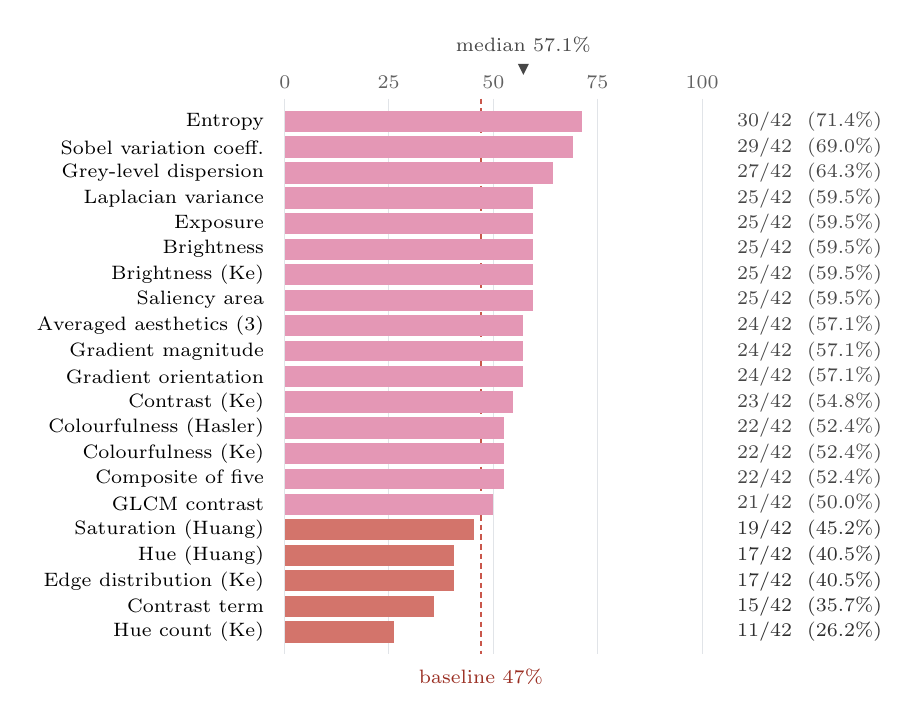
\begin{tikzpicture}[x=1cm,y=1cm,font=\scriptsize]
\draw[rulegray!30,line width=.3pt] (0.00,0.16) -- (0.00,-6.90);
\node[font=\scriptsize,text=black!62] at (0.00,0.36) {0};
\draw[rulegray!30,line width=.3pt] (1.32,0.16) -- (1.32,-6.90);
\node[font=\scriptsize,text=black!62] at (1.32,0.36) {25};
\draw[rulegray!30,line width=.3pt] (2.65,0.16) -- (2.65,-6.90);
\node[font=\scriptsize,text=black!62] at (2.65,0.36) {50};
\draw[rulegray!30,line width=.3pt] (3.97,0.16) -- (3.97,-6.90);
\node[font=\scriptsize,text=black!62] at (3.97,0.36) {75};
\draw[rulegray!30,line width=.3pt] (5.30,0.16) -- (5.30,-6.90);
\node[font=\scriptsize,text=black!62] at (5.30,0.36) {100};
\draw[accentred!85,line width=.9pt,dash pattern=on 2pt off 1.5pt] (2.49,0.16) -- (2.49,-6.90);
\node[anchor=east,font=\scriptsize] at (-0.14,-0.13) {Entropy};
\fill[focoauditado!45] (0,-0.27) rectangle (3.78,0.00);
\node[anchor=west,font=\scriptsize,text=black!72] at (5.62,-0.13) {30/42 \ (71.4\%)};
\node[anchor=east,font=\scriptsize] at (-0.14,-0.46) {Sobel variation coeff.};
\fill[focoauditado!45] (0,-0.59) rectangle (3.66,-0.32);
\node[anchor=west,font=\scriptsize,text=black!72] at (5.62,-0.46) {29/42 \ (69.0\%)};
\node[anchor=east,font=\scriptsize] at (-0.14,-0.78) {Grey-level dispersion};
\fill[focoauditado!45] (0,-0.92) rectangle (3.41,-0.65);
\node[anchor=west,font=\scriptsize,text=black!72] at (5.62,-0.78) {27/42 \ (64.3\%)};
\node[anchor=east,font=\scriptsize] at (-0.14,-1.11) {Laplacian variance};
\fill[focoauditado!45] (0,-1.24) rectangle (3.15,-0.97);
\node[anchor=west,font=\scriptsize,text=black!72] at (5.62,-1.11) {25/42 \ (59.5\%)};
\node[anchor=east,font=\scriptsize] at (-0.14,-1.43) {Exposure};
\fill[focoauditado!45] (0,-1.56) rectangle (3.15,-1.30);
\node[anchor=west,font=\scriptsize,text=black!72] at (5.62,-1.43) {25/42 \ (59.5\%)};
\node[anchor=east,font=\scriptsize] at (-0.14,-1.75) {Brightness};
\fill[focoauditado!45] (0,-1.89) rectangle (3.15,-1.62);
\node[anchor=west,font=\scriptsize,text=black!72] at (5.62,-1.75) {25/42 \ (59.5\%)};
\node[anchor=east,font=\scriptsize] at (-0.14,-2.08) {Brightness (Ke)};
\fill[focoauditado!45] (0,-2.21) rectangle (3.15,-1.94);
\node[anchor=west,font=\scriptsize,text=black!72] at (5.62,-2.08) {25/42 \ (59.5\%)};
\node[anchor=east,font=\scriptsize] at (-0.14,-2.40) {Saliency area};
\fill[focoauditado!45] (0,-2.54) rectangle (3.15,-2.27);
\node[anchor=west,font=\scriptsize,text=black!72] at (5.62,-2.40) {25/42 \ (59.5\%)};
\node[anchor=east,font=\scriptsize] at (-0.14,-2.73) {Averaged aesthetics (3)};
\fill[focoauditado!45] (0,-2.86) rectangle (3.03,-2.59);
\node[anchor=west,font=\scriptsize,text=black!72] at (5.62,-2.73) {24/42 \ (57.1\%)};
\node[anchor=east,font=\scriptsize] at (-0.14,-3.05) {Gradient magnitude};
\fill[focoauditado!45] (0,-3.18) rectangle (3.03,-2.92);
\node[anchor=west,font=\scriptsize,text=black!72] at (5.62,-3.05) {24/42 \ (57.1\%)};
\node[anchor=east,font=\scriptsize] at (-0.14,-3.37) {Gradient orientation};
\fill[focoauditado!45] (0,-3.51) rectangle (3.03,-3.24);
\node[anchor=west,font=\scriptsize,text=black!72] at (5.62,-3.37) {24/42 \ (57.1\%)};
\node[anchor=east,font=\scriptsize] at (-0.14,-3.70) {Contrast (Ke)};
\fill[focoauditado!45] (0,-3.83) rectangle (2.90,-3.56);
\node[anchor=west,font=\scriptsize,text=black!72] at (5.62,-3.70) {23/42 \ (54.8\%)};
\node[anchor=east,font=\scriptsize] at (-0.14,-4.02) {Colourfulness (Hasler)};
\fill[focoauditado!45] (0,-4.16) rectangle (2.78,-3.89);
\node[anchor=west,font=\scriptsize,text=black!72] at (5.62,-4.02) {22/42 \ (52.4\%)};
\node[anchor=east,font=\scriptsize] at (-0.14,-4.35) {Colourfulness (Ke)};
\fill[focoauditado!45] (0,-4.48) rectangle (2.78,-4.21);
\node[anchor=west,font=\scriptsize,text=black!72] at (5.62,-4.35) {22/42 \ (52.4\%)};
\node[anchor=east,font=\scriptsize] at (-0.14,-4.67) {Composite of five};
\fill[focoauditado!45] (0,-4.80) rectangle (2.78,-4.54);
\node[anchor=west,font=\scriptsize,text=black!72] at (5.62,-4.67) {22/42 \ (52.4\%)};
\node[anchor=east,font=\scriptsize] at (-0.14,-4.99) {GLCM contrast};
\fill[focoauditado!45] (0,-5.13) rectangle (2.65,-4.86);
\node[anchor=west,font=\scriptsize,text=black!72] at (5.62,-4.99) {21/42 \ (50.0\%)};
\node[anchor=east,font=\scriptsize] at (-0.14,-5.32) {Saturation (Huang)};
\fill[accentred!70] (0,-5.45) rectangle (2.40,-5.18);
\node[anchor=west,font=\scriptsize,text=black!82] at (5.62,-5.32) {19/42 \ (45.2\%)};
\node[anchor=east,font=\scriptsize] at (-0.14,-5.64) {Hue (Huang)};
\fill[accentred!70] (0,-5.78) rectangle (2.15,-5.51);
\node[anchor=west,font=\scriptsize,text=black!82] at (5.62,-5.64) {17/42 \ (40.5\%)};
\node[anchor=east,font=\scriptsize] at (-0.14,-5.97) {Edge distribution (Ke)};
\fill[accentred!70] (0,-6.10) rectangle (2.15,-5.83);
\node[anchor=west,font=\scriptsize,text=black!82] at (5.62,-5.97) {17/42 \ (40.5\%)};
\node[anchor=east,font=\scriptsize] at (-0.14,-6.29) {Contrast term};
\fill[accentred!70] (0,-6.42) rectangle (1.89,-6.16);
\node[anchor=west,font=\scriptsize,text=black!82] at (5.62,-6.29) {15/42 \ (35.7\%)};
\node[anchor=east,font=\scriptsize] at (-0.14,-6.61) {Hue count (Ke)};
\fill[accentred!70] (0,-6.75) rectangle (1.39,-6.48);
\node[anchor=west,font=\scriptsize,text=black!82] at (5.62,-6.61) {11/42 \ (26.2\%)};
\fill[black!72] (2.96,0.60) -- (3.10,0.60) -- (3.03,0.46) -- cycle;
\node[anchor=south,font=\scriptsize,text=black!72] at (3.03,0.62) {median 57.1\%};
\node[anchor=north,font=\scriptsize,text=accentred!80!black] at (2.49,-6.96) {baseline 47\%};
\end{tikzpicture}
\caption{Selected-segment retention under alternative implementations of the quality criterion. Only the scoring implementation is replaced; the bar is the percentage of the 42 redundancy-cluster representatives that survive the swap. \textbf{The median operation keeps 57.1 per cent of the decisions against a uniform-choice baseline of 47}, and the five in red keep fewer than chance. Retention ranges from 26 to 71 per cent. The clusters are shared across all twenty-one operations and the SIFT+BoVW one; \textbf{the frames are not}: the per-frame operations score one frame per second, while SIFT+BoVW runs its own internal key-frame selector.}
\label{fig:jusante}
\end{figure}



\clearpage
\begin{table}[!ht]
\centering
\caption{Origins, documented selection roles and evaluated implementations of the audited operations. Where origin and use fall in the same work the middle column says so, and the last column marks our own adaptations as such. The full inventory, with formulas and results files, is in Tables~\ref{tab:inventory} and~\ref{tab:trace}.}
\label{tab:reuse}
\footnotesize
\setlength{\tabcolsep}{4pt}
\renewcommand{\arraystretch}{1.12}
\begin{tabular}{@{}>{\raggedright\arraybackslash}p{2.35cm}>{\raggedright\arraybackslash}p{3.1cm}>{\raggedright\arraybackslash}p{3.2cm}>{\raggedright\arraybackslash}p{3.1cm}@{}}
\toprule
\rowcolor{headerblue}
\hd{Operation} & \hd{Origin and role there} & \hd{Documented use in selection} & \hd{Evaluated here} \\
\midrule
Edge distribution, hue count, contrast & \citet{ke2006highlevel}: features of a naive Bayes classifier for photo quality & \citet{srinivas2016rank} cite Ke for all three (\S3.1.3--3.1.5) and average them into a per-frame quality score & each term alone, plus the mean and an adapted classifier \\
\rowcolor{rowlight}Colourfulness in that same score & Swain and Ballard, by histogram intersection, as \citet{srinivas2016rank} state & \citet{srinivas2016rank}, \S3.1.1 & the Hasler expression instead, a declared substitution \\
Sharpness and brightness & \citet{korolkov2025keyframe}: two terms of a keyframe score & the same work, $0.7\,z(\mathrm{sharp})+0.3\,z(\mathrm{bright})$ & the published rule, with our normalization population stated \\
\rowcolor{rowlight}Grey-level dispersion & \citet{jeong2016static}: a badness term inside a cost multiplicative in cluster distance & the same work, within that objective & the isolated statistic, read in the increasing direction \\
Gradient magnitude, saliency, entropy, gradient orientation & \citet{qaroush2025diversity}: terms of four numbered objectives & the same work; two of the four objectives are not about technical quality & each term alone, and the visual-attention module of Eq.~20 \\
\bottomrule
\end{tabular}
\end{table}


\clearpage
%% GERADO por gera_tab_validacao.py. Nao editar a mao.
\begin{table}[p]
\centering
\caption{\textbf{What each source work reports as evidence for its own visual criterion.} Read from the full text of each paper; the excerpt is verbatim. \emph{Tests} names what the source puts to a test, which is not always the operation the later literature borrows. One of the eleven source works is not in our archive and carries no verdict here: \textbf{absence of a reading is not absence of validation}. It documents the clause carried on each band of the audit table in the main text.}
\label{tab:validation}
\scriptsize
\setlength{\tabcolsep}{2.6pt}
\renewcommand{\arraystretch}{0.96}
\begin{tabular}{@{}>{\raggedright\arraybackslash}p{2.1cm}>{\raggedright\arraybackslash}p{2.4cm}>{\raggedright\arraybackslash}p{3.5cm}>{\raggedright\arraybackslash}p{3.6cm}@{}}
\toprule
\rowcolor{headerblue}
\hd{Source} & \hd{Tests} & \hd{What it reports} & \hd{Verbatim excerpt} \\
\midrule
\rowcolor{perf5!35}\citet{ke2006highlevel} & \textbf{human judgement of the property} & community ratings on 60{,}000 photos as ground truth; per-feature precision--recall and a combined classifier at 27.8 per cent equal error, on the extremes only & \emph{``the photos have been rated by its community of users, giving us ground truth on the quality of each photo \,\ldots\, The top and bottom 10\% of the photos were extracted \,\ldots\, we chose to ignore the middle 80\%''} \\
\rowcolor{perf5!35}\citet{hasler2003colorfulness} & \textbf{human judgement of the property} & a psychophysical scaling experiment, seven categories, the expression fitted to the ratings at 94.0 per cent; the property is colourfulness & \emph{``We set up a psychophysical category scaling experiment, and ask people to rate images using 7 categories of colourfulness. We then fit a metric to the results''} \\
\rowcolor{perf2!45}\citet{srinivas2016rank} & the summary only & precision, recall and F of the selected keyframes against the ground-truth keyframes of seven open-video.org videos & \emph{``results are compared with the ground truth keyframes provided by open-video.org''} \\
\rowcolor{perf2!45}\citet{qaroush2025diversity} & the summary only & precision, recall and F1 of the extracted segments against reference summaries & \emph{``The evaluation focuses on comparing segments extracted by our system with those identified in ground truth summaries''} \\
\rowcolor{perf1!45}\citet{korolkov2025keyframe} & \textbf{neither the rule nor its weights} & weights set, not fitted; ablations vary segmentation parameters, and keyframes are judged by coverage and a qualitative review & \emph{``We set wsharp = 0.7, wbright = 0.3 to favor focused frames''} \\
\rowcolor{perf3!55}\citet{cakmak2025tripss} & the summary, with an ablation & TVSum20 and SumMe against human importance scores, with an ablation removing each modality & \emph{``Table 1 presents the results of an ablation study analyzing the contribution of each modality. Removing any single component''} \\
\bottomrule
\end{tabular}
\end{table}

%% GERADO por gera_tab_validacao.py. Nao editar a mao.
\begin{table}[p]
\centering
\caption{\textbf{Evidence reported by each source work, continued.} Columns as in the preceding table.}
\label{tab:validation_b}
\scriptsize
\setlength{\tabcolsep}{2.6pt}
\renewcommand{\arraystretch}{0.96}
\begin{tabular}{@{}>{\raggedright\arraybackslash}p{2.1cm}>{\raggedright\arraybackslash}p{2.4cm}>{\raggedright\arraybackslash}p{3.5cm}>{\raggedright\arraybackslash}p{3.6cm}@{}}
\toprule
\rowcolor{headerblue}
\hd{Source} & \hd{Tests} & \hd{What it reports} & \hd{Verbatim excerpt} \\
\midrule
\rowcolor{perf3!55}\citet{yang2024keyframe} & the summary, with an ablation & structural and feature ablations scored by F on SumMe over 15 annotations & \emph{``we conducted experiments on the SumMe dataset for structural ablation of the model and for feature ablation''} \\
\rowcolor{perf3!55}\citet{gygli2014summe} & the summary, with an ablation & f-measure against multiple human-created summaries per video, collected in a study with perception psychologists, plus an ablation measuring the gain of adding each feature to the set & \emph{``We evaluate our method using multiple `ground truth' summaries per video, which we acquired in a study in collaboration with perception psychologists''} \\
\rowcolor{perf3!55}\citet{jeong2016static} & the summary, with an optimisation ablation & summary-level human evaluation and precision/recall against labelled events, with a comparison against an optimisation-removed variant; the component-level claim here concerns the isolated grey-level statistic, which is not tested alone & \emph{``and (5) our method without the optimization procedure''} \textnormal{(Section 5, Experimental results)} \\
\rowcolor{perf2!45}\citet{huang2024aesthetic} & the summary only & Spearman and Kendall rank correlation against human annotations on four datasets, in canonical, augmentation and transfer setups & \emph{``we conduct an extensive evaluation of the models we developed by utilizing four distinct datasets: SumMe, TVSum, OVP, and YouTube \,\ldots\, we carry out our experiments using the dataset in three different setups: canonical (C), augmentation (A), and transfer (T)''} \textnormal{(Section IV.A, Experiments setup)} \\
\rowcolor{perf3!55}\citet{xu2024property} & the summary, with an ablation & F against summaries from five users on OVP, with an ablation of the frame-block length; no isolated test of the entities or of their weights & \emph{``All the scores are normalized to the interval [0, 1] and the higher value means the better''} \textnormal{(Section "Scoring the entities")} \\
\midrule
\bottomrule
\end{tabular}
\end{table}


\clearpage
%% GERADO por gera_tab_unidades.py -- nao editar a mao
\begin{table}[!ht]
\centering
\caption{Resampling unit per analysis, and the rival unit tested against it. Observations are nested, so the unit decides the width of every interval: the italic line under each row states the nesting, and \textbf{the declared unit follows from that nesting}, observations sharing content or a source entering the same block. Each interval is also recomputed under the rival unit, and the last column reports the outcome of that recomputation.}
\label{tab:unidades}
\footnotesize
\setlength{\tabcolsep}{4pt}
\begin{tabular}{@{}>{\raggedright\arraybackslash}p{1.0cm}>{\raggedright\arraybackslash}p{2.35cm}>{\raggedright\arraybackslash}p{1.6cm}>{\raggedright\arraybackslash}p{1.6cm}>{\raggedright\arraybackslash}p{4.1cm}@{}}
\toprule
\rowcolor{headerblue}
\hd{Block} & \hd{Analysis} & \hd{Declared unit} & \hd{Rival tested} & \hd{Outcome} \\
\midrule
\rowcolor{perf3!45}Block 01 & Paired difference, 800 pairs & segment block & the pair & \textbf{the two units give different widths; under the declared unit the interval is $[+29.8,+38.9]$}, and $[+30.4, +39.4]$ under the coarser source-aware block (12 blocks) \\
\rowcolor{perf3!45} & \multicolumn{4}{@{}>{\raggedright\arraybackslash\itshape}p{9.55cm}@{}}{\footnotesize 20 segments, 40 pairs each; pairs within a segment share content} \\
\cmidrule(lr){1-5}
\rowcolor{perf5!25}Block 01 & Strict accuracy, 800 pairs & topic block & the segment block & 11 of the 11 interval bounds reproduce under the declared unit, 2 under the rival \\
\rowcolor{perf5!25} & \multicolumn{4}{@{}>{\raggedright\arraybackslash\itshape}p{9.55cm}@{}}{\footnotesize the 20 segments come from 13 topic labels, 12 source-aware blocks after merging the two that share source videos} \\
\cmidrule(lr){1-5}
\rowcolor{perf5!25}Block 04 & In-domain floor, 42 clusters & topic block & the cluster & 3 of the 3 interval bounds reproduce under the declared unit, 1 under the rival \\
\rowcolor{perf5!25} & \multicolumn{4}{@{}>{\raggedright\arraybackslash\itshape}p{9.55cm}@{}}{\footnotesize the 42 clusters come from 19 topic labels, 18 source-aware blocks} \\
\cmidrule(lr){1-5}
\rowcolor{perf5!25}Block 04 & Output contrast, 42 clusters & topic block & the cluster & over eight seeds the bounds span $[-13.3, -11.2]$ and $[54.6, 55.5]$ under the declared unit, against $[-6.9, -5.8]$ and $[52.3, 52.9]$ under the rival \\
\rowcolor{perf5!25} & \multicolumn{4}{@{}>{\raggedright\arraybackslash\itshape}p{9.55cm}@{}}{\footnotesize the 42 clusters come from 19 topic labels, 18 source-aware blocks} \\
\cmidrule(lr){1-5}
\rowcolor{perf5!25}Block 04 & Regime contrast, 42 clusters & topic block & the cluster (exact McNemar) & the verdict holds under the declared unit ($p=.008$ against $p=.006$) \\
\rowcolor{perf5!25} & \multicolumn{4}{@{}>{\raggedright\arraybackslash\itshape}p{9.55cm}@{}}{\footnotesize the 12 discordant pairs fall in 9 topics; the null enumerates all $2^{9}$ block sign assignments} \\
\bottomrule
\end{tabular}
\end{table}


\clearpage
%% GERADO por gera_tab_inversoes.py -- nao editar a mao
\begin{table}[!ht]
\centering
\caption{Every operation--type cell below the 50 per cent chance floor, with its \emph{decisive} accuracy $W/(W+L)$, which leaves ties out of the denominator and therefore differs from the strict accuracy of the main tables wherever an operation ties. Significance is an exact sign-flip randomization with Holm across the 120 operation--type tests, reported for both nested units. Over the 20 broadcast segments, 22 of the 35 cells survive and $^{\dagger}$ marks the 13 that do not; over the 12 topic blocks, the more conservative unit, 11 survive and $^{\ddagger}$ marks the further 11 that fall. The 5 cells in which an operation is wrong on all one hundred pairs carry neither mark: they survive in both units. Counting ties inside the denominator instead of outside leaves the same 35 cells and the same 15 operations. Removing the two types aligned with an operation's own attribute, darkening and desaturation, leaves all 15 operations still inverting; removing white noise instead leaves 9. Dropping one segment at a time, all 15 keep inverting in every one of the 20 rounds. \textbf{Ties are unevenly spread}: 4 operations tie on at least one pair and the largest count is 81. Where ties are many, accuracy below 50 per cent does not by itself mean the degraded copy is preferred; the reading that does is correct against incorrect, which is what the sign-flip test compares. Dk = darkening, Mo = motion blur, Bl = Gaussian blur, H2 = H.264, Rs = rescaling, St = desaturation, Ns = white noise, Jp = JPEG.}
\label{tab:inversoes}
\footnotesize
\begin{tabular}{@{}>{\raggedright\arraybackslash}p{3.4cm}cc>{\raggedright\arraybackslash}p{5.6cm}@{}}
\toprule
\rowcolor{headerblue}
\hd{Operation} & \hd{Types} & \hd{Worst} & \hd{Cells below chance (\%)} \\
\midrule
Saliency area & 6 & \textcolor{accentred}{\textbf{10.0}} & Mo~29.0$^{\dagger}$, Bl~20.0$^{\dagger}$, Rs~21.0$^{\dagger}$, St~18.0$^{\ddagger}$, Ns~13.1$^{\ddagger}$, Jp~10.0$^{\ddagger}$ \\
\rowcolor{rowlight}Hue count (Ke) & 5 & \textcolor{accentred}{\textbf{4.2}} & Dk~21.7$^{\dagger}$, Mo~15.7$^{\dagger}$, Bl~12.3$^{\ddagger}$, Rs~14.1$^{\dagger}$, St~4.2$^{\ddagger}$ \\
Gradient orientation & 4 & \textcolor{accentred}{\textbf{0.0}} & Bl~26.0$^{\dagger}$, Rs~9.0, St~21.0$^{\dagger}$, Ns~0.0 \\
\rowcolor{rowlight}Gradient magnitude & 3 & \textcolor{accentred}{\textbf{0.0}} & St~23.0$^{\dagger}$, Ns~0.0, Jp~5.0 \\
Saturation & 3 & \textcolor{accentred}{\textbf{1.0}} & Dk~13.0$^{\ddagger}$, H2~15.0$^{\ddagger}$, Ns~1.0 \\
\rowcolor{rowlight}Entropy & 2 & \textcolor{accentred}{\textbf{0.0}} & H2~10.0$^{\ddagger}$, Ns~0.0 \\
Contrast (Ke) & 2 & \textcolor{accentred}{\textbf{10.3}} & St~31.6$^{\dagger}$, Ns~10.3$^{\ddagger}$ \\
\rowcolor{rowlight}Edge distribution & 2 & \textcolor{accentred}{\textbf{11.0}} & H2~11.0$^{\ddagger}$, Jp~31.0$^{\dagger}$ \\
Grey-level dispersion & 2 & \textcolor{accentred}{\textbf{22.0}} & St~22.0$^{\dagger}$, Ns~25.0$^{\dagger}$ \\
\rowcolor{rowlight}GLCM contrast & 1 & \textcolor{accentred}{\textbf{0.0}} & Ns~0.0 \\
Laplacian variance & 1 & \textcolor{accentred}{\textbf{0.0}} & Ns~0.0 \\
\rowcolor{rowlight}Gygli mean of three & 1 & \textcolor{accentred}{\textbf{3.0}} & Ns~3.0 \\
Colourfulness (Hasler) & 1 & \textcolor{accentred}{\textbf{3.0}} & Ns~3.0 \\
\rowcolor{rowlight}Colourfulness (Ke) & 1 & \textcolor{accentred}{\textbf{3.0}} & Ns~3.0 \\
Srinivas composite & 1 & 29.0 & Ns~29.0$^{\ddagger}$ \\
\bottomrule
\end{tabular}
\end{table}


\clearpage
%% GERADO por gera_tab_reimplementacao.py -- nao editar a mao
\begin{table}[!ht]
\centering
\caption{The SIFT+BoVW operation measured twice on the same 800 pairs: the reported run and an independent reimplementation of the same published operation under the same protocol. \textbf{The failure reproduces}: both collapse on white noise and JPEG, and both stay below the weakest published no-reference model at 80.8 per cent. They differ on desaturation, where the reported run inverts and the reimplementation does not, which is the one place where implementation detail changes a verdict. Red marks a cell below the 50 per cent chance floor.}
\label{tab:reimplementacao}
\scriptsize
\setlength{\tabcolsep}{2.2pt}
\begin{tabular}{@{}>{\raggedright\arraybackslash}p{2.6cm}cccccccc c@{}}
\toprule
\rowcolor{headerblue}
\hd{Run} & \hd{Darken} & \hd{Motion} & \hd{Blur} & \hd{H.264} & \hd{Rescale} & \hd{Satur.} & \hd{Noise} & \hd{JPEG} & \hd{Mean} \\
\midrule
Reported & 100 & 100 & 90 & 90 & 88 & \textcolor{accentred}{\textbf{39}} & \textcolor{accentred}{\textbf{8}} & \textcolor{accentred}{\textbf{6}} & \textbf{65.1} \\
\rowcolor{rowlight}Independent reimplementation & 100 & 100 & 92 & 94 & 93 & 56 & \textcolor{accentred}{\textbf{10}} & \textcolor{accentred}{\textbf{6}} & \textbf{68.9} \\
\bottomrule
\end{tabular}
\end{table}


\clearpage
%% GERADO por gera_tab_compostos.py -- nao editar a mao
\begin{table}[!ht]
\centering
\caption{\emph{Source works} lists the archive citekeys whose full text matches the terms of each combination. \textbf{A dagger marks the works whose use was verified against the source with a recorded excerpt}, held in \texttt{o\_que\_cada\_fonte\_valida.json} of the reproducibility package; the others are retrieval matches and are not evidence that the work adopts that combination, so the rows without a dagger are evaluated here as diagnostic configurations rather than as published algorithms. Screening of 19 diagnostic configurations built from attributes identified in the archive; \textbf{the aggregations are defined in this study}, not taken from a published algorithm. \emph{LBP} is the local binary pattern. \emph{Sens.} is the within-reference mean against the degradation level on KADID-10k under the $z$-score aggregation and \emph{Types} the count above $.50$ of 25. \emph{Gen.}\,($z$) is the direction-aligned correlation on KonIQ-10k as a magnitude, in the same configuration as \emph{Sens.}; \emph{Gen.}\,(ridge) is the generous variant, fitted outside the reference and reported separately. \textbf{Orientation comes from the data}, under the polarity-permissive rule of Section~3.3 of the main text, so a single-attribute row carries the opposite sign to Table~\ref{tab:literature} exactly when the declared direction contradicts the data. Eligibility uses the $z$-score configuration throughout; green marks the 1 row that clears the sensitivity gate.}
\label{tab:compostos}
\footnotesize
\setlength{\tabcolsep}{3pt}
\begin{tabular}{@{}>{\raggedright\arraybackslash}p{2.7cm}>{\raggedright\arraybackslash}p{3.55cm}ccccc@{}}
\toprule
\rowcolor{headerblue}
\hd{Combination} & \hd{Source works} & \hd{Sens.} & \hd{Types} & \hd{Gen. ($z$)} & \hd{Gen. (ridge)} & \hd{Eligible} \\
\midrule
colourfulness + Laplacian variance + LBP uniformity & \cite{cakmak2025tripss}$^{\dagger}$ & \textcolor{accentgreen}{\textbf{.524}} & 17 & .061 & .067 & no \\
Laplacian variance + LBP uniformity & \cite{singh2026subevent} & .439 & 15 & .080 & .082 & no \\
edge distribution & \cite{kannao2020semantic}, \cite{wang2012tag_localization} & .298 & 9 & .099 & .099 & no \\
spatial information & \cite{kishi2019correlation}, \cite{swain1991colorindexing}, \cite{taylor2017superresolution}, \cite{wu2026multimodal_gcl}, \cite{zhu2014keyobservation} & .251 & 13 & .513 & .513 & no \\
LBP uniformity + gradient magnitude & \cite{nandini2022edgelbp} & .189 & 8 & .177 & .007 & no \\
colourfulness & \cite{gygli2014creating}, \cite{hasler2003colorfulness}$^{\dagger}$ & .182 & 9 & .007 & .007 & no \\
LBP uniformity & \cite{barbieri2020webmedia}, \cite{barbieri2021content}, \cite{barbieri2021tese}, \cite{gharbi2019repeatability} & .175 & 12 & .205 & .205 & no \\
colourfulness + exposure & \cite{datta2006aesthetics} & .173 & 10 & .243 & .003 & no \\
edge distribution + hue count + Laplacian variance & \cite{ke2006highlevel}$^{\dagger}$ & .156 & 7 & .204 & .347 & no \\
colourfulness + edge distribution + hue count + saliency & \cite{srinivas2016rank}$^{\dagger}$, \cite{tang2013content} & .148 & 7 & .162 & .117 & no \\
exposure + Laplacian variance & \cite{korolkov2025keyframe}$^{\dagger}$ & .108 & 9 & .500 & .357 & no \\
colourfulness + gradient magnitude & \cite{qaroush2025diversity}$^{\dagger}$ & .108 & 11 & .296 & .066 & no \\
exposure & \cite{huang2024aesthetic}$^{\dagger}$ & .102 & 4 & .343 & .343 & no \\
GLCM contrast + entropy & \cite{yang2024keyframe}$^{\dagger}$ & .092 & 11 & .371 & .084 & no \\
LBP uniformity + saliency & \cite{qaroush2025centrality}, \cite{zhang2015aesthetics}, \cite{zhang2016georeferenced} & .089 & 9 & .071 & .277 & no \\
saliency & \cite{hussain2021mvs}, \cite{ngo2005graphmodeling}, \cite{nie2016perceptual}, \cite{park2025videograph}, \cite{zhang2015handheld}, \cite{zhang2015skimlets} & .075 & 3 & .333 & .333 & no \\
Laplacian variance & \cite{jeong2017static}, \cite{mittal2012brisque}, \cite{mittal2013niqe} & .047 & 9 & .601 & .601 & no \\
colourfulness + edge distribution & \cite{xu2024property}$^{\dagger}$ & .017 & 4 & .085 & .051 & no \\
LBP uniformity + entropy & \cite{chitrakala2025symmetry} & .009 & 8 & .007 & .285 & no \\
\bottomrule
\end{tabular}
\end{table}


%% --- o protocolo de identificacao das operacoes ---
\clearpage
%% GERADO por gera_tab_protocolo.py -- nao editar a mao
\begin{table}[!ht]
\centering
\caption{How the audited operations were identified, and what the protocol does and does not reach. The operations were not assembled from a database query, so the population of inference is the archive named in the first row and every count in this table is a count within it; no claim of exhaustive coverage is made. \textbf{The search instrument is itself measured against a manual reading, with the direction of the residual bias stated}, because a search whose accuracy is unknown cannot bound what it missed.}
\label{tab:protocolo}
\footnotesize
\setlength{\tabcolsep}{4pt}
\renewcommand{\arraystretch}{1.15}
\begin{tabular}{@{}>{\raggedright\arraybackslash}p{2.2cm}>{\raggedright\arraybackslash}p{6.6cm}>{\raggedright\arraybackslash}p{2.9cm}@{}}
\toprule
\rowcolor{headerblue}
\hd{Step} & \hd{What was done} & \hd{What it yielded} \\
\midrule
\textbf{Corpus} & Curated full-text archive on video and multi-document summarization and on image-quality assessment, searched on 5 September 2026. \textbf{Not a database query, so the population of inference is this archive.} & 186 PDFs \\
\rowcolor{rowlight}\textbf{Patterns} & One specific expression per operation family, never a bare word, so that \emph{contrast} alone does not match. Reference lists are cut before matching; a cut leaving under 40\,\% of the PDF is refused and the work enters whole. Spatial information counts only when its context window carries ITU, the SI/TI pair, \emph{index} or Sobel. & 13 patterns \\
\textbf{Instrument accuracy} & Measured against a manual reading of the sources. \textbf{The reading and the inventory were done by the same author}, so the estimates may be optimistic. \textbf{The assessed articles are not a random sample of the archive}: they are the source works of the inventory together with articles selected because their combinations came closest to passing, and the second group inflates false positives by construction, so precision is not an unbiased estimate for the archive as a whole. Cutting reference lists raised precision from .47 without moving recall. & recall .81, precision .63, on 21 articles \\
\rowcolor{rowlight}\textbf{Inventory inclusion rule} & An operation enters only if its source declares a direction for its own statistic and scores a single frame. \textbf{No operation without a declared direction was screened in.} The 3 that declare a direction and stay out are sequence-level: \texttt{qaroush\_movimento}, \texttt{qaroush\_ses}, \texttt{sobel\_cv}. & 15 of 24 mapped operations \\
\textbf{Coverage achieved} & Share of the operation mentions in the archive that the screened set covers. A mention is not an article: one PDF may name several. & 41 of 71 mentions (57.7\,\%) \\
\rowcolor{rowlight}\textbf{What is left out, and why} & \textbf{Of the 30 mentions outside, 25 were excluded under the inventory inclusion rule}, because the source specifies no direction (14) or no combination rule (11). & 25 of 30 excluded \\
\textbf{What the archive does instead} & The term sweep is an automated retrieval check over an archive assembled during the thesis research; it is not a systematic mapping, and a match implies no reading of the matched work. Works citing no dedicated no-reference quality model, and how many of those match the patterns of one of the audited operations. \textbf{These are term matches, not confirmed use}: they were not read individually, and the same search precision applies here. & 173 of 186 cite none; 33 of those matched an operation pattern \\
\bottomrule
\end{tabular}
\end{table}


% ⚠️ o suplementar cita 19 fontes na tabela de rastreio e nao tinha bibliografia
% ⭐ 21/09: a tabela taxonomica entra por ULTIMO de proposito. Inserida no
% meio, ela empurra o numero de todas as tabelas seguintes e quebra ponteiros
% do corpo que nada tem a ver com ela.
\begin{longtable}{@{}>{\raggedright\arraybackslash}p{6.0cm} cccc@{}}
\caption{\textbf{Class-term matches in the curated summarization archive.} It lists, work by work, which class terms the sweep found. A marker means the term sweep found the class in the body of the paper, with the bibliography removed. \textbf{This is triage, not a verdict}: a marker is a candidate for reading rather than a claim about the work. The term sweep is an automated retrieval check over an archive assembled during the thesis research; it is not a systematic mapping, and a match implies no reading of the matched work. The precision measured for the archive sweep recorded in Table~\ref{tab:protocolo} was measured on a different term set and is not claimed for this sweep. Class~4 is marked only when the text names the selection use, distance to a cluster centre or representativeness; cosine similarity alone is not counted, because in summarization it serves redundancy and clustering far more often than quality.}\\
\label{tab:taxonomy_works}\\
\toprule
\rowcolor{headerblue}
\hd{Work} & \hd{C1} & \hd{C2} & \hd{C3} & \hd{C4} \\
\midrule
\endfirsthead
\toprule
\rowcolor{headerblue}
\hd{Work} & \hd{C1} & \hd{C2} & \hd{C3} & \hd{C4} \\
\midrule
\endhead
\bottomrule
\endfoot
\cite{basavarajaiah2019compressed} & $\bullet$ & $\bullet$ &  & $\bullet$ \\
\rowcolor{rowlight}\cite{chitrakala2025symmetry} & $\bullet$ & $\bullet$ &  & $\bullet$ \\
\cite{jeong2016static} & $\bullet$ & $\bullet$ &  & $\bullet$ \\
\rowcolor{rowlight}\cite{ji2019quasc} & $\bullet$ & $\bullet$ &  & $\bullet$ \\
\cite{qaroush2025centrality} & $\bullet$ & $\bullet$ &  & $\bullet$ \\
\rowcolor{rowlight}\cite{singh2026subevent} & $\bullet$ & $\bullet$ &  & $\bullet$ \\
\cite{xu2024property} & $\bullet$ &  & $\bullet$ & $\bullet$ \\
\rowcolor{rowlight}\cite{yang2024keyframe} & $\bullet$ & $\bullet$ &  & $\bullet$ \\
\cite{avila2011vsumm} & $\bullet$ &  &  & $\bullet$ \\
\rowcolor{rowlight}\cite{barbieri2020webmedia} & $\bullet$ & $\bullet$ &  &  \\
\cite{barbieri2021content} & $\bullet$ & $\bullet$ &  &  \\
\rowcolor{rowlight}\cite{barbieri2021tese} & $\bullet$ & $\bullet$ &  &  \\
\cite{beserra2020evaluating} & $\bullet$ & $\bullet$ &  &  \\
\rowcolor{rowlight}\cite{beserra2023multimodal} & $\bullet$ & $\bullet$ &  &  \\
\cite{cakmak2025tripss} & $\bullet$ & $\bullet$ &  &  \\
\rowcolor{rowlight}\cite{chasanis2008spectral} & $\bullet$ &  &  & $\bullet$ \\
\cite{chu2015video_cosummarization} &  & $\bullet$ &  & $\bullet$ \\
\rowcolor{rowlight}\cite{gharbi2017modularity} & $\bullet$ & $\bullet$ &  &  \\
\cite{gharbi2019repeatability} & $\bullet$ & $\bullet$ &  &  \\
\rowcolor{rowlight}\cite{gygli2014creating} & $\bullet$ &  &  & $\bullet$ \\
\cite{gygli2014summe} & $\bullet$ &  &  & $\bullet$ \\
\rowcolor{rowlight}\cite{hussain2021mvs} & $\bullet$ & $\bullet$ &  &  \\
\cite{kishi2019correlation} & $\bullet$ & $\bullet$ &  &  \\
\rowcolor{rowlight}\cite{messaoud2021deepqamvs} & $\bullet$ &  &  & $\bullet$ \\
\cite{nandini2022edgelbp} & $\bullet$ & $\bullet$ &  &  \\
\rowcolor{rowlight}\cite{over2008trecvid} & $\bullet$ & $\bullet$ &  &  \\
\cite{panda2017diversity} & $\bullet$ & $\bullet$ &  &  \\
\rowcolor{rowlight}\cite{qaroush2025diversity} & $\bullet$ & $\bullet$ &  &  \\
\cite{saqib2018mme} & $\bullet$ & $\bullet$ &  &  \\
\rowcolor{rowlight}\cite{sidiropoulos2011temporal} & $\bullet$ & $\bullet$ &  &  \\
\cite{song2015tvsum} &  & $\bullet$ &  & $\bullet$ \\
\rowcolor{rowlight}\cite{srinivas2016rank} & $\bullet$ &  &  & $\bullet$ \\
\cite{trojahn2021temporal} & $\bullet$ & $\bullet$ &  &  \\
\rowcolor{rowlight}\cite{wang2012tag_localization} & $\bullet$ & $\bullet$ &  &  \\
\cite{wu2020dyngcn} & $\bullet$ &  &  & $\bullet$ \\
\rowcolor{rowlight}\cite{wu2026multimodal_gcl} & $\bullet$ &  &  & $\bullet$ \\
\cite{xie2008affinity} & $\bullet$ & $\bullet$ &  &  \\
\rowcolor{rowlight}\cite{zhang2015aesthetics} & $\bullet$ &  &  & $\bullet$ \\
\cite{zhang2015handheld} & $\bullet$ & $\bullet$ &  &  \\
\rowcolor{rowlight}\cite{barbara2025prompts_summaries} &  &  &  & $\bullet$ \\
\cite{fu2010multiview} & $\bullet$ &  &  &  \\
\rowcolor{rowlight}\cite{hong2011beyond_search} &  & $\bullet$ &  &  \\
\cite{hua2025v2xum} & $\bullet$ &  &  &  \\
\rowcolor{rowlight}\cite{huang2024aesthetic} & $\bullet$ &  &  &  \\
\cite{islam2025multimodal} &  & $\bullet$ &  &  \\
\rowcolor{rowlight}\cite{ji2018mvs_hds} & $\bullet$ &  &  &  \\
\cite{kadam2025systematic} &  & $\bullet$ &  &  \\
\rowcolor{rowlight}\cite{kalkhorani2024beyond_frame} &  & $\bullet$ &  &  \\
\cite{korolkov2025keyframe} & $\bullet$ &  &  &  \\
\rowcolor{rowlight}\cite{lei2019framerank} &  &  &  & $\bullet$ \\
\cite{li2010videommr} &  & $\bullet$ &  &  \\
\rowcolor{rowlight}\cite{ngo2005graphmodeling} & $\bullet$ &  &  &  \\
\cite{nie2016perceptual} & $\bullet$ &  &  &  \\
\rowcolor{rowlight}\cite{otani2019rethinking} &  &  &  & $\bullet$ \\
\cite{panda2016embedded_multiview} & $\bullet$ &  &  &  \\
\rowcolor{rowlight}\cite{panda2017collaborative} &  & $\bullet$ &  &  \\
\cite{park2025videograph} & $\bullet$ &  &  &  \\
\rowcolor{rowlight}\cite{shao2010complex_graph} &  & $\bullet$ &  &  \\
\cite{soares2018topicsegment} &  & $\bullet$ &  &  \\
\rowcolor{rowlight}\cite{wang2009multidoc} &  & $\bullet$ &  &  \\
\cite{zhang2013geospace} &  & $\bullet$ &  &  \\
\rowcolor{rowlight}\cite{zhang2015skimlets} & $\bullet$ &  &  &  \\
\cite{zhang2016georeferenced} & $\bullet$ &  &  &  \\
\rowcolor{rowlight}\cite{zhou2018drdsn} &  &  &  & $\bullet$ \\
\cite{zhu2014keyobservation} & $\bullet$ &  &  &  \\
\rowcolor{rowlight}\cite{zhu2023topicaware} & $\bullet$ &  &  &  \\
\cite{apostolidis2021survey} &  &  &  &  \\
\rowcolor{rowlight}\cite{argaw2024scaling} &  &  &  &  \\
\cite{duygulu2004autodoc} &  &  &  &  \\
\rowcolor{rowlight}\cite{kaushal2020visiocity} &  &  &  &  \\
\cite{lee2025llmvs} &  &  &  &  \\
\rowcolor{rowlight}\cite{li2012balanced_avmmr} &  &  &  &  \\
\cite{li2025lgrln} &  &  &  &  \\
\rowcolor{rowlight}\cite{li2025spivg} &  &  &  &  \\
\cite{lin2024videogenic} &  &  &  &  \\
\rowcolor{rowlight}\cite{moraes2022subjectivity} &  &  &  &  \\
\cite{panda2016camera_network} &  &  &  &  \\
\rowcolor{rowlight}\cite{panda2017multiview_surveillance} &  &  &  &  \\
\cite{panda2017sparse_topic} &  &  &  &  \\
\rowcolor{rowlight}\cite{park2020sumgraph} &  &  &  &  \\
\cite{rojaschaves2024videosage} &  &  &  &  \\
\rowcolor{rowlight}\cite{wu2019mvsgcn} &  &  &  &  \\
\cite{yeh2025gcn_compressed} &  &  &  &  \\
\rowcolor{rowlight}\cite{yu2026deep} &  &  &  &  \\
\cite{zhao2026graphvsum} &  &  &  &  \\
\end{longtable}


%% ⭐ 21/09: PROCEDIMENTO INFERENCIAL, movido do corpo. O corpo tinha dez paginas de
%% metodo, das quais boa parte era detalhe de execucao — transformadas de Fisher, Steiger,
%% margens, familias de multiplicidade, hardware. Isso pertence aqui: o corpo diz o QUE foi
%% feito e sob que unidade, e este bloco diz COMO. Entra no FIM para nao empurrar a
%% numeracao de nenhuma tabela.
\clearpage
\section*{Inferential procedure in full}\label{sup:inference}

\paragraph{Units of analysis, and which one each result uses.} Observations are nested and
the unit is reported per analysis rather than once for the design. Strict accuracy on the
constructed pairs is block-bootstrapped by topic; the paired score difference by segment;
KADID sensitivity by reference image; the application by news topic. Observations that
share content or a source enter the same block, which is the segment for pairs cut from
one segment and the topic for clusters drawn from one news topic. All bootstraps use
$10^4$ resamples and seed 42. Table~\ref{tab:unidades} recomputes every interval under the
rival unit, and Table~\ref{tab:inversoes} reports per-cell significance under both the
segment and the topic block.

\paragraph{Exact tests.} Per-cell significance uses an exact sign-flip randomization whose
null enumerates all $2^{b}$ block sign assignments for $b$ blocks, with Holm over the 120
operation--type tests. Disagreement counts between the complete-operation and
matched-input regimes are compared by an exact McNemar test over the 42 paired clusters
and, because those clusters come from 19 topics and McNemar treats them as independent, by
the same block sign-flip over topics, which enumerates all $\mcnAtrib{}$ assignments the
discordant pairs admit across \mcnBlocos{} topics.

\paragraph{External association.} Spearman correlation against MOS or DMOS. Confidence
intervals for KonIQ and CLIVE use the Fisher transform; KADID intervals and paired
differences use reference-block bootstrap. Dependent correlations on the same images use
Steiger's statistic~\citep{steiger1980comparing}. The operational equivalence margin is
$|\Delta\rho^{*}|<.02$, chosen as the largest association difference treated as
practically negligible for this diagnostic rather than as a literature-wide standard; the
paired difference and interval are reported so stricter margins can be applied. The
multiplicity family contains all 630 pairwise contrasts among 36 evaluated scores
(17 methods and 19 ablations); Bonferroni correction gives $\alpha=0.05/630$ and critical
$|z|=3.95$. The accuracy, consistency and linearity triad after the monotonic mapping
required by ITU-T P.1401 is in Table~\ref{tab:p1401}~\citep{itu_p1401}.

\paragraph{The application estimand.} For each operation the application selects one
representative per cluster. If $y_c$, $l_c$ and $h_c$ are the selected, lowest and highest
reference scores in cluster $c$, and $\bar y=|C|^{-1}\sum_{c\in C}y_c$ with $\bar l$ and
$\bar h$ defined analogously, the estimand is $100(\bar y-\bar l)/(\bar h-\bar l)$: a
ratio of means, not an average of independently rescaled clusters. Zero-range clusters are
undefined for per-cluster position and are counted explicitly. \textbf{The primary interval resamples the \fusBlocos{} source-aware blocks that the \senBlocos{} topic labels of the application collapse to} and retains the clusters of each block: the two labels that share source videos count as one. This is the same grouping \emph{rule} the constructed pairs use, on different data, so it yields a different \emph{number} of blocks there (\invBlocos{}, from \invRotulos{} labels). Two sensitivity analyses accompany it, one resampling the \senBlocos{} separate topic labels and one resampling clusters within each sampled label. Raw branch-score differences,
mean per-cluster position, selected-maximum rate, range distributions and exclusions of
the smallest 10\% and 25\% of ranges are in Table~\ref{tab:e2e15}.

\paragraph{Degradation parameters.} Eight degradations at five levels: Gaussian blur,
white noise, darkening, JPEG compression, low-bitrate H.264 transcoding, a
downscale-and-restore round trip at five factors, horizontal motion blur and progressive
desaturation, the last using $S'_{\ell}=\operatorname{clip}(\alpha_{\ell}S,0,255)$ with
$\alpha_{\ell}\in\{0.75,0.55,0.35,0.18,0.05\}$. H.264 is applied to the frame sequence;
the others are frame-based. Exact parameters are in Table~\ref{tab:degradation}.

\paragraph{Environment.} Experiments ran on one NVIDIA RTX~4060 GPU (8~GB). NR-IQA
implementations use the PyIQA toolbox~\citep{chen2022pyiqa}; SIFT uses OpenCV and the
vocabulary uses mini-batch $K$-means with $K=300$ and \texttt{random\_state=42}. Q-Align is
quantized to 4-bit NormalFloat with double quantization and FP16 compute to fit the
GPU~\citep{dettmers2023qlora}; no numerical equivalence to unquantized inference is
assumed. Frames are decoded once and cached, and latency is re-measured in one software
environment after ten warm-up and sixty timed iterations.

\clearpage
%% ⭐ 23/09 (parecer v8, §3): a lista dos dezessete, que o corpo promete e o
%% revisor nao achou. Entra no FIM de proposito: inserir no meio renumeraria
%% os ponteiros sem ancora do corpo, calado.
%% GERADO por gera_tab_dezessete.py -- nao editar a mao
\begin{table}[!ht]
\centering
\caption{The seventeen operations of the auxiliary comparison in Section~4.2 of the main text. \textbf{\emph{Accuracy} is the same quantity the source-level synthesis (Section~4.7) of the main text reports}: strict accuracy in per cent, ties counted as errors, averaged over all eight transformation types, on the 800 original--transformed comparisons. \emph{Aligned-excluded} is a second aggregation of the same measurement, reported here because it appears elsewhere in this supplement: it drops ties from the denominator and averages only over the types not aligned by construction with the operation, which differ from row to row, so it rests on the smaller number of comparisons in the last column. \emph{Excluded} names those types and \emph{Pairs} counts the comparisons they leave, \textbf{before ties are removed}, so the denominator that aggregation actually uses is smaller again wherever the operation ties. \textbf{The two aggregations are not interchangeable}: relative to the canonical column the second is higher for some operations, lower for others and equal where neither ties nor alignment applies. Both columns are derived from the same pair-level measurements. A double dagger marks the two sequence operations, which the isolated-frame inclusion rule excludes from the directional inventory and which enter only this auxiliary comparison. Under the canonical aggregation 8 of the seventeen fall below SIFT+BoVW at 65.1\% and the median is 66.0\%; over the 15 of the directional inventory alone the count is 6 and the median 74.8\%. Identifiers in \texttt{typewriter} are function names in the released package, kept verbatim so each row can be matched to the code that produced it.}
\label{tab:dezessete}
\footnotesize
\setlength{\tabcolsep}{3.5pt}
\begin{tabular}{@{}>{\raggedright\arraybackslash}p{3.0cm}>{\raggedright\arraybackslash}p{2.5cm}rr>{\raggedright\arraybackslash}p{1.35cm}r@{}}
\toprule
\rowcolor{headerblue}
\hd{Identifier} & \hd{Operation} & \hd{Acc.} & \hd{Aligned-ex.} & \hd{Excluded} & \hd{Pairs} \\
\midrule
\rowcolor{rowwhite}\texttt{qaroush\_\allowbreak{}saliencia} & Saliency & 33.4 & 33.5 & --- & 800 \\
\rowcolor{rowlight}\texttt{ke\_\allowbreak{}hue\_\allowbreak{}count} & Hue count (Ke) & 36.8 & 39.0 & --- & 800 \\
\rowcolor{rowwhite}\texttt{qaroush\_\allowbreak{}go} & Gradient orientation & 53.9 & 53.9 & --- & 800 \\
\rowcolor{rowlight}\texttt{sobel\_\allowbreak{}cv}$^{\ddagger}$ & Sobel variation coefficient & 59.6 & 56.3 & Bl, Mo & 600 \\
\rowcolor{rowwhite}\texttt{ke\_\allowbreak{}edge\_\allowbreak{}distribution} & Edge distribution & 63.4 & 64.3 & Bl, Mo & 600 \\
\rowcolor{rowlight}\texttt{qaroush\_\allowbreak{}movimento}$^{\ddagger}$ & Motion & 63.5 & 61.7 & Mo & 700 \\
\rowcolor{rowwhite}\texttt{qaroush\_\allowbreak{}entropia} & Entropy & 63.8 & 63.8 & --- & 800 \\
\rowcolor{rowlight}\texttt{huang\_\allowbreak{}saturacao} & Saturation & 64.9 & 59.9 & St & 700 \\
\rowcolor{rowwhite}\texttt{qaroush\_\allowbreak{}gm} & Gradient magnitude & 66.0 & 66.0 & --- & 800 \\
\rowcolor{rowlight}\texttt{ke\_\allowbreak{}contraste} & Contrast (Ke) & 74.8 & 72.2 & Dk & 700 \\
\rowcolor{rowwhite}\texttt{laplacian\_\allowbreak{}var} & Laplacian variance & 76.4 & 68.5 & Bl, Mo & 600 \\
\rowcolor{rowlight}\texttt{contraste\_\allowbreak{}variancia} & Grey-level dispersion & 79.6 & 76.7 & Dk & 700 \\
\rowcolor{rowwhite}\texttt{glcm\_\allowbreak{}contraste} & GLCM contrast & 79.9 & 77.0 & Dk & 700 \\
\rowcolor{rowlight}\texttt{gygli\_\allowbreak{}media\_\allowbreak{}crua} & Averaged aesthetics (Gygli) & 83.8 & 67.5 & Bl, Dk, Mo, St & 400 \\
\rowcolor{rowwhite}\texttt{hasler\_\allowbreak{}colorfulness} & Colourfulness (Hasler) & 85.2 & 83.1 & St & 700 \\
\rowcolor{rowlight}\texttt{ke\_\allowbreak{}colorfulness} & Colourfulness (Ke) & 85.2 & 83.1 & St & 700 \\
\rowcolor{rowwhite}\texttt{srinivas\_\allowbreak{}quality} & The mean rule (Srinivas) & 87.0 & 74.5 & Bl, Dk, Mo, St & 400 \\
\bottomrule
\end{tabular}
\end{table}


\clearpage
%% GERADO por gera_tab_reducao.py -- nao editar a mao
\begin{table}[!ht]
\centering
\caption{Replacing the score by a simpler quantity, on the 42 application clusters and 83 distinct segments. \emph{$\rho$} is the Spearman correlation with the published score; \emph{Same choice} counts the clusters whose selected representative is unchanged when the quantity replaces the score, and \emph{Same order} the ordered pairs it preserves. \textbf{The descriptor count reproduces every choice}, so the operation is that count. \textbf{How many key frames the selector retains does not}: it tracks the score at $+.177$ and reproduces barely more than half the choices, while keypoints per frame tracks it at $+.599$. The count is therefore carried by detail per frame rather than by the number of frames. Segment duration ranges from 8.1 to 187.6 seconds and does not predict the score ($\rho=+.165$) or the count ($\rho=+.175$). Marks: $^{\ast}$ $p<.05$, $^{\mathrm{ns}}$ not significant; all other rows have $p<.01$.}
\label{tab:reducao}
\footnotesize
\setlength{\tabcolsep}{4pt}
\begin{tabular}{@{}>{\raggedright\arraybackslash}p{2.9cm}>{\raggedright\arraybackslash}p{4.6cm}ccc@{}}
\toprule
\rowcolor{headerblue}
\hd{Quantity} & \hd{What it is} & \hd{$\rho$} & \hd{Same choice} & \hd{Same order} \\
\midrule
\rowcolor{rowwhite}Descriptor count & the number of SIFT descriptors the key frames yield & $+.995$ & 42\,/\,42 & 63\,/\,63 \\
\rowcolor{rowlight}Keypoints per frame & descriptor count divided by frames retained & $+.599$ & 29\,/\,42 & 44\,/\,63 \\
\rowcolor{rowwhite}Frames retained & how many key frames the selector keeps & $+.177$$^{\mathrm{ns}}$ & 23\,/\,42 & 39\,/\,63 \\
\rowcolor{rowlight}Score per frame & the score divided by frames retained & $+.722$ & --- & --- \\
\rowcolor{rowwhite}Score per descriptor & the mean rarity weight of Eq.~3 of the main article & $+.115$$^{\mathrm{ns}}$ & --- & --- \\
\bottomrule
\end{tabular}
\end{table}


\bibliography{references}




%% ⭐ 28/09 (parecer + decisao do Jader): o benchmark de MODELO saiu do corpo (4.5 e 4.6)
%% para ca, para o artigo principal ficar na pergunta da auditoria. O texto e o mesmo que
%% estava no corpo, com os numeros pelas mesmas macros. Secao sem numero e sem tabela, no
%% fim: nao renumera nenhuma Tabela S.
\clearpage
\section*{Model eligibility and output quality}\label{sup:benchmark}

This section carries the model-level detail summarized in Sections 4.5 and 4.6 of the main
text: how robust the eligible set is, the in-domain floor model by model, a common-reference
comparison, and whether substituting the scorer improves the output according to DOVER.

Three methods are eligible: LIQE, QualiCLIP and CLIP-IQA$+$, and no single one is
best on both axes. The set is unchanged when the generalization threshold varies from .60
to .65 or the coverage cut from 12 to 22 types; at .55 MUSIQ is added and at .70 only LIQE
remains. The universal unseen-database clause is what separates them: TOPIQ,
MUSIQ, DBCNN and HyperIQA are strong on the unseen authentic database and fall to between
.462 and .556 on KADID. Part of the gap between SIFT+BoVW and the eligible methods on KADID is a change of regime: the SIFT+BoVW form adds a term proportional to $\log_{10}(K/N)$ in the descriptor count, positive over the small broadcast clusters and negative over a database of thousands of images, so moving to KADID changes how the score is built; the derivation of that term is given in this supplement.

On the in-domain floor the three pass with overlapping topic-block intervals, LIQE
agreeing with Q-Align, the in-domain reference of the model set, on
\pisoLiqeAcertos{} of \pisoDe{} clusters ($\kappa_{\mathrm{uniform}}=\pisoLiqeKappa{}$,
95\% CI \finLiqe{} over the \fusBlocos{} source-aware blocks). The SIFT+BoVW operation
agrees on \pisoSiftAcertos{}, only \pisoAcima{} decisions above the uniform expectation,
and its interval crosses chance ($\pisoSiftKappa{}$, \finSift{}).
%% ⛔ 27/09 (parecer, B): o piso e computado contra o Q-Align para TODOS, mas o
%% SIFT+BoVW e operacao derivada da literatura, e a 3.3 declara o LIQE como
%% referencia dessas. Reportar so contra o Q-Align deixava a medida fora da
%% referencia que o proprio metodo lhe atribui. Os dois numeros sao medidos.
Against LIQE, the reference the protocol assigns to the literature-derived
operations, the same operation agrees on \subResta{} of \pisoDe{}
($\kappa_{\mathrm{uniform}}=\subKappa{}$), and that interval crosses chance as well. Several literature-derived operations meet this condition on unmodified broadcasts despite failing both external ones, and \pisoFrageis{} lose that pass when one topic is removed. Keeping the \senBlocos{} topic labels apart leaves both verdicts unchanged (\senLiqe{} and \senSift{}).

%% ⛔ 21/09: esta declaracao foi cortada por engano ao compactar, e sem ela os dois
%% conjuntos de dez (o do piso e o dos candidatos) diferem sem que o corpo diga por que.
An auxiliary comparison places every scorer against one common reference, and its
group is not the complete-case candidate set. Because LIQE is the designated reference for
the literature-derived operations, it cannot also be a candidate there, so the group
comprises the nine other complete-case candidates and ARNIQA in its place. All ten meet
the condition, with median normalized agreement \pisoKapMod{} against \pisoKapOp{} for the
literature-derived operations.

The sensitivity axis alone already differs between the two benchmarks. Applied
to the constructed broadcast pairs, the same rule keeps the mean threshold of .50 and
rescales the coverage clause in proportion, from 15 of KADID's 25 distortion types to 5
of the 8 types built here; it admits six of the fifteen, and none meets it on
both benchmarks.  Cost is
secondary but not negligible: the SIFT+BoVW operation takes 182~s per cluster and LIQE
1.9~s, a system-level figure that includes sampling and pooling.

\paragraph{Output quality with DOVER.} Its technical branch, DOVER-T, is the output measure.
The selected segments are rewrapped as common 5-frame-per-second MP4 inputs and evaluated
using the official view decomposition and paired seed; Table~\ref{tab:methods_supp} specifies fragment sampling.
For selected reference score $y_c$ and the lowest and highest reference scores $l_c,h_c$ in each cluster, the achievable-range position is
\begin{equation}
100\,\frac{\bar y-\bar l}{\bar h-\bar l},\qquad
\bar y=|C|^{-1}\sum_{c\in C}y_c,
\label{eq:sup_globalrange}
\end{equation}
with analogous definitions for $\bar l$ and $\bar h$. This ratio of means is distinct from averaging separately normalized cluster positions. It is defined when $\bar h>\bar l$ and expresses range points on a reference model's scale, not a percentage of human quality.

On the complete substitution, the global achievable-range position of
Equation~\eqref{eq:sup_globalrange}, not the branch score itself, rises from
\dovImplantada{}\% to \dovLiqe{}\%, $+\dovDif{}$ range points, but its block interval
$\finDovComp{}$ and hierarchical interval $\dovICHier{}$ both cross zero, so no
population-level effect is confirmed. Under matched inputs, with at most ten uniformly spaced
frames and mean pooling for both, the DOVER-T contrast is $\dovCasado{}$ range points with
both intervals positive (block $\finDovCas{}$; hierarchical $\dovCasadoHier{}$), and
$\dovCasadoCru{}$ on the raw branch score. Block intervals merge the two topic labels that
share source videos; hierarchical intervals resample clusters within the \senBlocos{}
separate labels, and no verdict differs under the separate-label grouping.

\end{document}
